%\documentclass[11pt]{scrartcl}


%ronny
\documentclass[12pt]{scrreprt}

\usepackage{primaer}
\usepackage[backend=bibtex]{biblatex}
\usepackage[babel,german=quotes]{csquotes}
\usepackage{setspace}
\usepackage{subcaption}
\usepackage{txfonts}
\usepackage{algorithm}
\usepackage[ngerman]{babel}
%\usepackage{algorithm}
\usepackage{algorithmic}
\usepackage{tikz}
\usepackage{hyperref}
\usepackage{listings}
\usetikzlibrary{trees}
\usetikzlibrary{shapes}
\usetikzlibrary{automata}
\usetikzlibrary{backgrounds}
\usetikzlibrary{plotmarks}
\usetikzlibrary{arrows}
%ende ronny

\bibliography{literatur}
\defbibheading{bibliography}[\bibname]{%
\chapter{#1}%
\markboth{#1}{#1}}

\AtEveryBibitem{% Clean up the bibtex rather than editing it
 \clearfield{doi}
 \clearfield{isbn}
 \clearfield{issn}
 %\clearlist{location}

 
  \ifboolexpr
    {
      test { \ifentrytype{article} }
      or
      test { \ifentrytype{inproceedings} }
    }
    {\clearfield{url}}
    {}%
}

\definecolor{javared}{rgb}{0.6,0,0} % for strings
\definecolor{javagreen}{rgb}{0.25,0.5,0.35} % comments
\definecolor{javapurple}{rgb}{0.5,0,0.35} % keywords
\definecolor{javadocblue}{rgb}{0.25,0.35,0.75} % javadoc

\lstset{basicstyle=\ttfamily}

%\geometry{a4paper,left=25mm,right=50mm, top=13mm, bottom=20mm}
%\geometry{a4paper,right=50mm,left=25mm}
\newcommand{\ff}{\triangleright}
\newcommand{\pref}[1]{\mathit{pref{#1}}}
\renewcommand{\min}{\mathit{Min}\;}

\newtheorem{def1}{Definition}
\newtheorem{satz}{Satz}
\newtheorem{lem}{Lemma}
\newtheorem{bew}{Beweis} 
\newtheorem{gleich}{Gleichung}[section]
\newtheorem{eigen}{Eigenschaft}
\newtheorem{folg}{Folgerung}
\theoremstyle{remark}
\newtheorem{beispiel}{Beispiel}

\author{Robert Hartmann}
\title{Vergleich von SQL-Anfragen: Theorie und Implementierung in Java}
\date{27. August 2013}
\parindent 0pt
\begin{document}

\pagestyle{empty}

\begin{center}

{\Large\sc Masterarbeit}

\vspace{1.25cm}

{\fontsize{22}{22}\selectfont Vergleich von SQL-Anfragen\\Theorie und Implementierung in Java}

\vspace{1.25cm}

{\Large\sc

Robert Hartmann

\vspace{.15cm}

Betreuer: Prof. Dr. Stefan Brass

\vspace{.15cm}

24. September 2013

}

\vspace{10.5cm}

\begin{tabular}{c}
	
\includegraphics[height=15ex]{Bilder/siegel}
\end{tabular}

\vspace{0.5cm}

\rule{.7\textwidth}{.40pt}

\vspace{.2cm}

{\large\sc

martin-luther-universit"at halle-wittenberg

}

\end{center}

\cleardoublepage


%\include{dedication}



\onehalfspacing
\vspace*{10mm}
{\huge \textbf{Zusammenfassung}}\\\\
In der Lehre möchte man häufig SQL-Anfragen des Lernenden mit einer hinterlegten Musterlösung vergleichen, um deren Äquivalenz zu zeigen. Diese Arbeit beschäftigt sich mit dem semantischen Vergleich zweier SQL-Anfragen. Dabei wird ein Standardisierungsverfahren für SQL-Anfragen entwickelt, welches mit Hilfe des Datenbankschemas SQL-Anfragen legal umformt und dabei erreicht, dass semantisch gleiche Anfragen nach der Umformung auch syntaktisch gleich sind. Schlägt dieses Verfahren fehl, so wird in einem weiteren Verfahren mit realen Daten geprüft, ob die Anfragen tatsächlich ungleich sind. Diese Verfahren werden in einem Prototypen in Java implementiert und bilden eine Lernplattform, die dem Nutzer per Java Server Pages in einem Webbrowser zur Verfügung gestellt wird. Metadaten und Struktur der beiden SQL-Anfragen werden ausgewertet und der Nutzer erhält dadurch detailliertes Feedback, um so seine Fehler leichter zu bemerken.\newline\newline\newline\newline\newline
{\huge \textbf{Abstract}}\\\\
In university teaching one often want to compare a students sql query to a sample solution to show the equivalence of them. This thesis is about the semantic comparison of two SQL queries. We develop a method of standardization that legally rewrites a SQL query with the help of the database schema. If two SQL queries are semantically equal they shall be syntactically equal as well after the standardization. If this method fails we try to prove that the two queries are not semantically equal. Therefore we execute both queries on a real database and check their results. These methods are implemented in a Java prototype and form a learning platform that contains an interface built with Java Server Pages so the user can access it via web browser. The structure and meta information of the user query and the sample solution query are being compared and evaluated to give the user a detailed feedback on his query.

\pagestyle{plain}

\singlespacing
\tableofcontents

\onehalfspacing

\chapter{Einleitung / Motivation}
\label{chap:introduction}
%einleitung

SQL (structured query language) ist eine Datenbanksprache, die in relationalen Datenbanken zum Definieren, Ändern und Abfragen von Datenbeständen benutzt wird. Basierend auf relationaler Algebra und dem Tupelkalkül, ist sie einfach aufgebaut und ähnelt der englischen Sprache sehr, was Anfragen deutlich verständlicher gestaltet. SQL ist der Standard in der Industrie wenn es um Datenbankmanagementsysteme (DBMS) geht. Zu bekannten Vertretern gehören Oracle Database von Oracle, DB2 von IBM, PostgreSQL von der PostgreSQL Global Development Group, MySQL von der Oracle Corporation und SQLServer von Microsoft.

Die Umsetzung von SQL als quasi-natürliche Sprache erlaubt es Anfragen so zu formulieren, dass sie allein mit dem Verständnis der natürlichen Sprache verständlich sind. Dieser Umstand hat auch dazu geführt, dass heutzutage relationale Datenbanksysteme mit SQL beliebt sind und häufig eingesetzt werden. 
Dies führt allerdings auch dazu, dass es mehrere, syntaktisch unterschiedliche, Anfragen geben kann, welche semantisch identisch sind. Manche sehen sich dabei ähnlich, andere Anfragen kann man nur nach Umformen ineinander überführen. 

\section{Motivation}

Ein gängiges Mittel um herauszufinden, ob zwei SQL-Anfragen das gleiche Ergebnis liefern, ist es die Anfragen auf einer Datenbank mit vorhandenen Daten auszuführen. Dies bildet jedoch lediglich Indizien für eine mögliche semantische Gleichheit. Da man die zwei zu vergleichenden Anfragen nur auf einer endlichen Menge von Datenbankzuständen testen kann, ist nie ausgeschlossen, dass nicht doch ein Zustand existiert, der unterschiedliche Ergebnisse liefert. Weiterhin stehen solche Testdaten nur im begrenzten Umfang zur Verfügung oder Daten müssten händisch eingetragen werden bzw. von freien Internetdatenbanken beschafft werden. Dies kostet Zeit und Arbeitskraft, welche im universitärem Umfeld meist beschränkt ist. So haben Hochschulen immer weniger Geld für Tutoren oder Hilfskräfte, was die Zeit der wenigen Mitarbeiter umso wertvoller macht.

Durch diese Situation sind Professoren immer öfter dazu gezwungen mehr Lehre und weniger Forschung zu betreiben, was aber offensichtlich auch keine gute Lösung ist. Häufig werden dem Lernenden Übungsaufgaben gestellt, die dieser dann innerhalb einer Frist bearbeitet und abgibt. Diese müssen dann kontrolliert und wieder ausgehändigt werden. Bei diesem Prozess kann nur schwer auf die einzelnen Fehler der Studenten eingegangen werden. Auch ist es ein zusätzlicher Zeitaufwand herauszufinden, welche Fehler besonders häufig auftreten. Des weiteren sind manche Lernende auch gewillt mehr zu üben, um sich gerüstet für eine Klausur zu fühlen. Andere möchten gezielt ein Thema üben, welches sie noch nicht gut beherrschen. All das ist mit Übungsaufgaben und Übungen innerhalb der Hochschule schwer zu erreichen. 

Das Programm, welches im Rahmen dieser Arbeit entwickelt wird, soll helfen all diese Probleme zu lösen. Es soll mit wenig Aufwand für den Mitarbeiter der Universität möglich sein neue Aufgaben in das System einzupflegen. Durch Abspeicherung sämtlicher Lösungsversuche des Lernenden können einzelne Aufgaben vom Dozenten durch das Programm auf häufig auftretende Fehler untersucht werden. Damit kann in der Übung gezielt besprochen werden, was noch oft falsch gemacht wird.

\section{Aufgabenstellung}

Nach der theoretischen Ausarbeitung soll ein Programm entwickelt werden, welches in der Lage ist zwei SQL-Anfragen zu vergleichen. Dieser Vergleich soll, im ersten Schritt, lediglich mit Musterlösung, Lösung des Lernenden und Datenbankschema möglich sein. Im zweiten Schritt werden die zwei Anfragen auch gegen reale Daten geprüft. Da die Fehlermeldung des Standardparsers von SQL sehr allgemein gehalten sind, ist es auch wünschenswert, dass das Programm konkretere Hinweis- und Fehlermeldung ausgibt, als es der Standard SQL-Parser vermag. Weiterhin sollen die Fehlermeldung sich konkret auf den Unterschied von Musterlösung zur Lösung des Lernenden beziehen. Damit das Programm möglichst plattformunabhängig bedient werden kann, soll es als Webseite auf einem Server zur Verfügung gestellt werden. Da als Programmiersprache Java gewählt wurde, bieten sich die JSP (java server pages) an, welche auf den java-servlets basieren.

Wir bezeichnen zwei SQL-Anfragen als syntaktisch äquivalent, wenn die zwei Anfragen syntaktisch identisch sind. Dies ist der Fall wenn beide Anfragen als Zeichenketten in jedem Buchstaben übereinstimmen. Zwei SQL-Anfragen sind dagegen semantisch äquivalent, wenn beide Anfragen auf allen Datenbankzuständen einer Datenbank stets die selben Tupel zurückliefern. Zu Bemerken ist hierbei, dass zwei semantisch äquivalente Anfragen keinesfalls syntaktisch äquivalent sein müssen, wie das folgende Beispiel zeigt:

\begin{figure}
\begin{verbatim}
Anfrage 1: SELECT * FROM emp WHERE sal > 1000
Anfrage 2: SELECT * FROM emp e WHERE 1000 < e.sal
\end{verbatim}
\caption{Beispiel: semantisch, aber nicht syntaktisch, äquivalente Anfragen}
\end{figure}

Wie bereits beschrieben erfolgt der Vergleich zweier SQL-Anfragen zweistufig. Können beide Anfragen durch Standardisierungen in syntaktisch äquivalente Anfragen umgeformt werden, so sind sie auf jeden Fall auch semantisch äquivalent. Das Umformen durch Standardisierung stellt daher eine hinreichende Bedingung für die Gleichheit der SQL-Anfragen dar. Es gibt aber auch Anfragen, die nicht syntaktisch, aber dennoch semantisch äquivalent sind. Solche Anfragen können in einigen Fällen strukturell sehr unterschiedlich und dennoch semantisch äquivalent sein. Mit dem Vorgehen im ersten Schritt würden wir solche Anfragen nicht aneinander anpassen. In diesem Fall fahren wir mit dem zweiten Schritt fort. In diesem werden beide Anfragen auf realen Datenbanken ausgeführt. Sind beide Anfragen semantisch äquivalent, so müssen beide die selben Ergebnistupel liefern. Ist dies nicht der Fall, so ein Gegenbeispiel für die semantische Äquivalenz gefunden. Das Liefern von gleichen Ergebnissen beider Anfragen auf dem selben Datenbankzustand ist also eine notwendige Bedingung für die semantische Äquivalenz. Im Kapitel \ref{chap:ausblick} wird noch auf Anfragen eingegangen, die weder im Schritt 1 bestätigt noch im Schritt 2 abgelehnt werden konnten. 


Ein mögliches Haupteinsatzgebiet ist die Lehre. Dort soll es möglich sein Untersuchungen des Lernfortschritts von Studenten oder anderen Interessierten, die den Einsatz von SQL erlernen möchten, durchzuführen. So kann das Programm dem Lernenden nicht nur sinnvolle Hinweise bei einer falschen Lösung geben, sondern auch erläutern, ob die gefundene Lösung eventuell zu kompliziert gedacht war. Des Weiteren ist es aufgrund der zentralisierten Serverstruktur möglich, Lösungsversuche des Lernenden zu speichern und eine persönliche Lernerfolgskurve anzeigen zu lassen. Damit hätten Studenten und Lehrkräfte die Möglichkeiten Lernfortschritte zu beobachten und Problemfelder (etwa JOINs) zu erkennen um diese dann gezielt zu bearbeiten. Dozenten könnten so im Zuge der Vorbereitung der Übung oder Vorlesung sich die am häufigsten aufgetretenen Fehler anzeigen lassen, um diese dann mit den Studenten direkt zu besprechen.

Damit ist es möglich eine Lernplattform aufzubauen, die dem Studenten mehrere Auswertungsinformationen über seinen Lernerfolg und seine Lösung deutlich macht. So kann die Lehrkraft eine Aufgabe mit samt Musterlösung und Datenbankschema hinterlegen und der Student kann daraufhin seine Lösungsversuche in das System eintragen. Durch sinnvolles Feedback ist es ihm möglich beim Üben direkt zu lernen. Weiterhin kann man eine solche Plattform auch für Tutorien oder Nachhilfe überall da benutzen, wo SQL gelernt wird. Vorteile hier wären, dass man mehrere verschiedene Aufgaben stellen kann ohne viel Zeit beim Einpflegen von neuen Aufgaben verbringen zu müssen.

Weitere Einsatzgebiete könnten sich im Unternehmen befinden. So könnte man bei einer geplanten Umstrukturierung oder Erzeugung von Datenbanken bereits Anfragen prüfen und vergleichen, bevor man sich u.U. teure Testdaten kauft oder Daten migrieren muss.

\section{Aufbau der Arbeit}

Im vorherigen Abschnitt haben wir geklärt warum es eine Notwendigkeit für das Thema SQL-Vergleich gibt. Zu dem wurde geklärt, was das Ziel der Arbeit ist. 

Im Kapitel \ref{chap:forschung} betrachten wir den aktuellen Forschungsstand zur Thematik Lernplattformen und SQL. Das Ergebnis dieser Arbeit soll ein Produkt sein, was hauptsächlich in der Lehre eingesetzt wird. Daher ist es wichtig bereits vorhandene Lernplattformen zu untersuchen. Dabei interessieren uns insbesondere Gemeinsamkeiten und Unterschiede zu unserer Arbeit. Wir werden feststellen, dass jede Plattform auf eine Feinheit spezialisiert ist und andere Punkte dann eine untergeordnete Rolle spielen. Weiterhin ist diese Bestandsaufnahme wichtig, da sie uns aufzeigen kann, wie man mögliche Ansätze miteinander verknüpft. Dieser Gedanke wird im Kapitel \ref{chap:ausblick} genauer erläutert.

Die Fragestellung ``Sind zwei SQL-Anfragen äquivalent'' ist nicht entscheidbar. Aus diesem Grund klären wir im Kapitel \ref{chap:theorie} wie wir den Entscheidungsprozess angehen wollen, sodass zumindest eine Teilmenge von SQL-Anfragen bearbeitet werden kann. Wir klären also zunächst, wie unser Programm vorgehen wird. Danach werden die einzelnen Schritte, die zum Vergleich notwendig sind, erklärt und besprochen. Dabei diskutieren wir für einzelne Teilschritte auch mehrere Herangehensweisen. Weiterhin werden wir alle möglichen Analyseschritte theoretisch untermauern, auch wenn nicht alle davon im Programm umgesetzt werden können. Mehr dazu im Abschnitt >>Grenzen des Parsers<<. Alle später umgesetzten Algorithmen werden in diesem Kapitel vorgstellt, erarbeitet und diskutiert.


Im nachfolgenden Kapitel \ref{chap:software} beschreiben wir die verwendete Software. Neben der üblichen Beschreibung der verwendeten Software, wird insbesondere auf den verwendeten Parser und die Java-Servelets eingegangen. Zu klären ist hier wie genau der Parser funktioniert und was er nicht kann. Daraus leitet sich eine gewisse Beschränkung in der praktischen Umsetzung ab. Da wir im vorherigen Kapitel allerdings alle theoretischen Betrachtungen ausführlich erläutert haben, stellt es kaum ein Problem dar, die vorgestellten Algorithmen auf einen anderen Parser zu übertragen. Ein weiterer Aspekt dieses Kapitels ist es, dem Leser klar zu machen wie Java-Servelets funktionieren und wie genau wir sie für unser Programm einsetzen.

In Kapitel \ref{chap:praxis} wird der Aufbau des Programms geklärt und erläutert. Dabei gehen wir den strukturellen Aufbau durch und klären, wie einzelne Aspekte aus Kapitel \ref{chap:theorie} umgesetzt werden konnten. Weiterhin klären wir, was aufgrund gewisser Beschränkungen nicht umsetzbar war. Wir diskutieren die Struktur des Programms hier eingehend auf Konzepte der Softwaretechnik, wie \mbox{z. B.} Wartbarkeit, Erweiterbarkeit usw.

%TODO: Ergebnisse und Ausblick (zusammenfassen)

\section{Produkt}

Es wurde im Rahmen der Aufgabenstellung ein Programm entwickelt, das es erlaubt zwei SQL-Anfragen miteinander zu vergleichen. Dazu wurde eine Lernplattform auf Basis von Java-Servlets geschaffen. Der Lernende meldet sich an der Plattform an und wählt eine Kategorie aus. Nun wird ihm eine Sachaufgabe gestellt und ein Datenbankschema angezeigt. Er soll nun daraus eine SQL-Anfrage formulieren, die die Aufgabenstellung löst. Dabei bekommt der Lernende Feedback von dem Programm. Dies schließt sowohl Hinweise als auch konkrete Fehlermeldungen ein. Hat der Lernende die Aufgabe bereits mehrfach bearbeitet, so kann er sich seine vorherigen, eingesandten Lösungen anschauen und seinen Lernerfolg leicht verfolgen. Das Programm zeigt auch an, in welcher Kategorie der Lernende noch große Defizite hat.

Der Dozent hat das Programm vorher einmalig mit einer Reihe von Aufgaben bestückt. Dazu gibt der Dozent eine textuelle Beschreibung der Aufgabe, eine oder mehrere SQL-Anfragen als Musterlösungen, ein Datenbankschema und optional eine Datenbank an, auf der Beispieldaten vorhanden sind. 

Das Programm läuft im Wesentlichen in zwei Schritten ab. Im ersten Schritt versucht es die zwei Anfragen miteinander zu vergleichen, ohne den Einsatz von externen Daten. Gelingt dies, ist gezeigt, dass die Lösung des Studenten mit der Musterlösung übereinstimmt. Das Programm meldet Erfolg und zeigt eventuell abweichende Komplexitätsmaße an. Mehr dazu im Abschnitt [].

Schlägt der erste Schritt fehl, wird die Anfrage des Lernenden auf der angegebene Datenbank verarbeitet und mit den Ergebnistupeln verglichen, die die Musterlösung liefern. Sind beide in allen Beispielzuständen gleich, so wird dem Dozenten gemeldet, dass eine eventuelle neue Musterlösung gefunden wurde. Diese ist strukturell so unterschiedlich, dass sie nicht auf die bisherige Musterlösung angepasst werden konnte. Wir können in einem solchen Fall nicht mit Sicherheit sagen, ob die Lösung falsch oder richtig ist, da dieses Problem im Allgemeinen nicht entscheidbar ist. Daher muss ein Prüfer solche Lösungen noch einmal manuell kontrollieren.

Schlägt aber auch der zweite Schritt fehl, so können wir sicher sein, dass die Lösung des Lernenden falsch ist. Das Programm meldet dann eine Fehlermeldung sowie mögliche Hinweise, was der Lernende falsch gemacht haben könnte.




\chapter{Forschungsstand und Einordnung}
\label{chap:forschung}
\section{Einleitung}

Die Idee, SQL-Anfragen von Lernenden automatisch zu kontrollieren, ist nicht völlig neu. Weil eine Auswertung über den Standard SQL-Parser nicht sehr umfangreich ist und es bei semantischen Fehlern kein sinnvolles Feedback gibt, sind bereits einige Ansätze veröffentlicht worden, die es sich zum Ziel gemacht haben eine SQL-Anfrage näher zu analysieren. Verschiedene Projekte beschäftigen sich dabei \mbox{z. B.} mit dem Aufdecken von semantischen Fehlern. Andere Plattformen konzentrieren sich auf den Lernerfolg, den der Student erreichen soll, und analysieren die Art der Fehler des Lernenden. Damit erreicht man eine Zuteilung von passenderen Aufgaben, sodass der Lernende weder gelangweilt noch überfordert ist. %matchamking

In diesem Abschnitt möchten wir die bereits existierenden Ansätze auf diesem Gebiet kurz betrachten, um dann diese Arbeit dann einordnen zu können.

\section{SQL-Tutor}

In \cite{sqltut1} beschreibt Antonija Mitrovic ein Lernsystem, was SQL-Tutor genannt wird. Nach Auswahl einer Schwierigkeitsstufe wird dem Studenten ein Datenbankschema und eine Sachaufgabe vorgelegt. Der Student hat nun ein Webformular in dem sich für jeden Teil der SQL-Anfrage ein Eingabefeld befindet. So werden die Anteile \verb|SELECT|, \verb|FROM|, \verb|WHERE|, \verb|ORDER BY|, \verb|GROUP BY| sowie \verb|HAVING| einzeln eingetragen.

Der SQL-Tutor analysiert nun die Anfrage des Studenten und gibt spezifisches Feedback. Dabei wird nicht nur geklärt, ob die Anfrage korrekt ist, sondern auch, was bei einer falschen Eingabe genau fehlerhaft ist. Das reicht von konkreten Hinweisen auf den spezifischen Teil der Anfrage bis hin zu eindeutigen Hinweisen wie >>Musterlösung enthält einen numerischen Vergleich mit der Spalte a, ihre Lösung enthält aber keinen solchen Vergleich<<.

Umgesetzt wird dieses Programm durch 199 fest einprogrammierte Constraints. Dadurch ist es potentiell möglich bis zu 199 spezifische Hinweismeldungen für den Studenten bereitzustellen. Das reicht von syntaktischen Analysen wie >>The SELECT Clauses of all solutions must not be empty<< bis hin zu semantischen Analysen, gepaart mit Wissen über die Domain (Datenbankschema und Musterlösung), bei denen die Lösung des Studenten mit der Musterlösung und dem Datenbankschema verglichen wird. Insbesondere versucht der SQL-Tutor Konstrukte wie numerische Vergleiche mit gewissen Operatoren in der Lösung des Studenten zu finden, wenn diese in der Musterlösung auftauchen. Auch komplexere Constraints, die sicherstellen, dass bei einem numerischen Vergleich \verb|a > 1| das gleiche ist wie \verb| a >= 0| sind vorhanden. 

Allerdings gibt es auch hier Schwächen. Da der verwendete Algorithmus die Constraints nach einander abarbeitet, kann es zu unnötigen Analysen der Anfrage kommen und damit auch zu einem unnötigen Zeitaufwand. Nach eigenen Tests werden manche äquivalente Bedingungen nicht erkannt. So wird \verb|a < 0| für richtig, aber \verb|0 > a| für falsch gehalten. Ähnlich verhält es sich, falls eine der Argumente des Vergleichs das Ergebnis einer Unterabfrage ist. Die Constraints sind fest einprogrammiert und nicht von der Anfrage abhängig und damit genügt es für eine neue Aufgabe Text und Musterlösung einzulesen. 

Der SQL-Tutor lässt außerdem den eingesendeten Lösungsvorschlag auf einer SQL-Datenbank mit Testdaten laufen und vergleicht die Tupel mit den Antworttupeln, die man mit der gespeicherten Musterlösung erhält.

\subsection*{Abgrenzung zum SQL-Tutor}

Der Grundgedanke des SQL-Tutors überschneidet sich durchaus mit dem Ansatz dieser Arbeit. Ein Grundpfeiler des SQL-Tutors ist es, dem Studenten detailliertes Feedback über seine semantischen und syntaktischen Fehler zu geben. Das Programm was im Zuge dieser Arbeit entsteht soll weniger semantische Fehler analysieren, als viel mehr versuchen zwei SQL-Anfragen zu vergleichen, unabhängig davon wie sie aufgeschrieben sind. Des Weiteren bedient sich der SQL-Tutor einer Testdatenbank mit realen Testdaten. Unser Programm soll nur das Datenbankschema kennen und ohne Daten bestimmen, ob zwei Anfragen das gleiche Ergebnis liefern. Erst in einem optionalen zweiten Schritt prüfen wir in unserem Programm die Anfragen auf konkreten Daten. Hat aber bereits unser erster Schritt ein positives Ergebnis gemeldet, dann ist der zweite Schritt unnötig. Der SQL-Tutor operiert allerdings zur Ermittlung der Übereinstimmung nur auf Testdaten. Bei ungünstig gewählten Testdaten kann es passieren, dass der Eindruck entsteht zwei Anfragen wären gleich, obwohl sie es nicht sind. Entstehen kann dies, weil auf den vorhanden Testdaten zufällig beide Anfragen die gleichen Ergebnisse liefern.

\section{SQL-Exploratorium}

Im Artikel \cite{explora1} werden SQL-Lernplattformen in zwei Kategorien eingeteilt. Zum einen existieren Plattformen, welche durch Multimedia versuchen dem Lernenden einzelne Bestandteile der Sprache SQL bildlich darzustellen. Hierfür werden meist Websites mit Multimediainhalten erstellt. Die zweite Kategorie beinhaltet Software, welche die Lösung eines Lernenden analysiert und konkrete Hinweismeldungen gibt. Dazu zählt auch der eben beschriebene SQL-Tutor.

Das SQL-Exploratorium macht es sich nun zur Aufgabe die beiden Ansätze zu verbinden und stellt sich dabei hauptsächlich verwaltungstechnische Fragen wie \mbox{z. B.} 

\begin{itemize}
\item Wie ermögliche ich dem Studenten Zugriff auf verschiedene Lernsysteme ohne sich mehrfach einloggen zu müssen?
\item Wie können Lernerfolge in einem System einem anderen nutzbar gemacht werden?
\item Wie kann man aus mehreren Logfiles der eingereichten Lösungen eines Studenten von unterschiedlichen Systemen einen Wissensstand des Studenten ableiten?
\end{itemize}

Da die Fragen als solche eher unwichtig für diese Arbeit sind, betrachten wir im Folgenden welche einzelnen Plattformen für das SQL-Exploratorium genutzt werden.

\subsection{Interactive Examples}

Über eine Schnittstelle, die sich WebEX nennt, hat der Student Zugriff auf insgesamt 64 Beispielanfragen. Wählt man eine Anfrage aus können Teile davon in einer Detailansicht geöffnet werden. Dem Studenten wird dann ausführlich erklärt, was die einzelnen Teile der Anfrage genau bewirken. Sowohl die Beispielanfragen, als auch die Hinweise sind manuell erzeugt und abgespeichert. Hier wird nichts automatisch generiert, daher ist dieses Projekt nicht relevant für die Arbeit. Der Lernerfolg des Studenten wird hier über die ein >>click-log<< geführt, das bedeutet es wird aufgezeichnet, was der Student wann und in welcher Reihenfolge angeklickt hat. So ist es \mbox{z. B.} möglich herauszufinden welche Teile einer bestimmten Anfrage besonders interessant für den Lernenden sind.

\subsection{SQL Knowledge Tester}

Der SQL Knowledge Tester, im Nachfolgendem SQL-KnoT genannt, konzentriert sich darauf Anfragen eines Studenten zu analysieren. Dabei wird dem Studenten zur Laufzeit eine Frage generiert. Dabei werden vorhandene Datenbankschemata in einer bestimmten Art und Weise verknüpft und Testdaten so wie eine Frage für den Studenten generiert. Dies geschieht mit fest einprogrammierten 50 Templates, die in der Lage sind über 400 Fragen zu erzeugen. Zu jeder Frage werden zur Laufzeit Testdaten für die relevanten Datenbanken erzeugt. Ausgewertet wird die Anfrage des Studenten dann, in dem die zurückgelieferten Tupel der Studentenanfrage verglichen werden mit den Tupeln, welche die Musterlösung erzeugt. 

\subsection*{Abgrenzung zur Arbeit}

Erwähnenswert ist, dass initial keine Daten existieren. Wie beim Ansatz dieser Arbeit existieren nur Datenbankschemata. Die Daten und auch die Aufgabe an den Studenten werden aus Templates generiert. Die Auswertung erfolgt dann allerdings durch den Vergleich der zurückgelieferten Tupel der Muster- und Studentenanfrage. Hierbei kann wieder das Problem auftreten, dass für beide Anfragen die erzeugten Testdaten die gleichen Tupel zurückliefern, es aber bei einem anderen Zustand sein kann, dass sich die Tupelmengen unterscheiden. 

Der Ansatz vom SQL-KnoT ist durchaus interessant, wird aber in dieser Arbeit nicht weiter ausgeführt, da wir in dieser Arbeit keine Testdaten erzeugen möchten. Wir benutzen vielmehr Beispieldaten als optionalen zweiten Schritt.

\subsection{Weiteres}

\subsubsection{Adaptive Navigation for SQL Questions}

Hierbei handelt es sich nur um ein Tool, was aufgrund früherer Antworten des Studenten, diesem möglichst passende neue Fragen vorlegen soll. Dieser Teil des SQL-Exploratoriums dient also dazu, den Wissensstand des Studenten festzustellen und ist für diese Arbeit daher unerheblich.

\section{WIN-RBDI}

Das Programm WINRBDI, welches in \cite{winrbdi1} beschrieben wird verfolgt einen weiteren, interessanten Ansatz. Anstelle von fest vorgegebenen Demoanfragen, wird die eingegebene Anfrage zunächst in esql eingebettet. Die Ausführung der Anfrage wird dann schrittweise durchgeführt. Der Student hat also die Möglichkeit die Anfrage im Schrittmodus, ähnlich eines Debugger, oder im Fortsetzen-Modus auszuführen. Im Schrittmodus wird jeder Teilschritt der Abarbeitung der Anfrage aufgezeigt. Es werden temporär erzeugte Tabellen angegeben sowie auch eine Erklärung welcher Teil der Anfrage für den aktuellen Abarbeitungsschritt verantwortlich ist. So soll es dem Studenten möglich sein, die unmittelbaren Konsequenzen seiner SQL-Anfrage für die Abarbeitung zu begreifen. 

Des Weiteren hilft dieser Ansatz dem Studenten die Abarbeitung einer Anfrage zu Visualisieren, indem von der WHERE Klausel betroffene Spalten markiert werden. Dies hilft gerade Lernanfängern bei der Visualisierung von Konzepten wie JOINs.

\subsection*{Abgrenzung zur Arbeit}

Dieser Ansatz hebt sich von den bisherig betrachteten Ansätzen ab. Hier wird dem Studenten durch eine Visualisierung der Ausführung der Anfrage versucht deutlich zu machen, welche Teile der formulierten Anfrage was genau bewirken. Für den Lernerfolg des Studenten ist dies sicherlich hilfreich, zumal eine Visualisierung stets hilft Zusammenhänge zu begreifen. Diese Arbeit verfolgt allerdings ein anderes Ziel, da sie zwei SQL-Anfragen miteinander vergleicht und nicht versucht die Abarbeitung einer Anfrage zu visualisieren.

\section{SQLLint}

>>SQLLint<<, ein Semantik-Prüfer für SQL-Anfragen, beschäftigt sich mit semantischen Fehlern in SQL-Anweisungen, welche unabhängig vom Datenbankzustand auftreten. Dabei behandelt das Projekt Anfragen, von denen man ohne Kenntnis der Aufgabenstellung sagen kann, dass sie, in der vorliegenden Form, nicht beabsichtigt sind. Dies ist wahrscheinlich, wenn man \mbox{z. B.} Teile aus der Anfrage herausstreichen kann ohne die Funktion der Anfrage zu verändern.  Das Problem besteht darin, dass aktuelle DBMS-Systeme solche Anweisungen ohne Fehler- oder Warnmeldung ausführen. Der Nutzer, also insbesondere der lernende Nutzer, ist somit kaum in der Lage überhaupt zu bemerken, dass es einen Fehler in seiner Anfrage gab. Eine generelle Frage der Gültigkeit solcher SQL-Anfragen ist nicht entscheidbar, dennoch macht es sich SQLLint zur Aufgabe eine große, typische Teilmenge von SQL-Anfragen zu bearbeiten. Ziel des Projektes ist es, mit semantischen Warn- und Fehlermeldungen, die Codeentwicklung zu beschleunigen und die Anzahl der Fehler darin zu verringern.

Ein nicht unwesentlicher Ansatz des Projektes ist es, solche Fehlermeldungen in der Lehre einzusetzen. In \cite{sqllint1} wird auch deutlich gemacht, das eine Motivation dieses Projektes aus typischen Fehlern von Studenten entspringt. So wurde im selben Artikel aufgeführt, dass semantische Fehler bei Lernenden am häufigsten auftreten. Unter den drei häufigsten semantischen Fehlern befinden sich: fehlende JOIN Bedingung, (zu) viele Duplikate, unnötiger JOIN. Diese Fehler machen bereits ca. 37 Prozent der semantischen Fehler aus.

Weiterhin fällt auf, dass die Anzahl syntaktischer Fehler mit fortschreitendem Schwierigkeitsgrad der SQL-Anfrage steigen, aber die Anzahl semantischer Fehler nahezu unabhängig von jenem Schwierigkeitsgrad ist. Einfache Anfragen haben sogar zwei mal mehr semantische Fehler als syntaktische Fehler. Siehe dazu \emph{Abbildung 4} in \cite{sqllint1}.

\subsection{Algorithmus zum Finden von inkonsistenten Bedingungen}

Die Algorithmen im SQLLint-Projekt sollen inkonsistente Bedingungen finden. Dieses Probleme ist allerdings im Allgemeinen unentscheidbar. Dennoch ist es möglich Teilmengen von Anfragen anzugeben, für die man die Konsistenz algorithmisch Entscheiden kann. Folgende Ausführungen zum Algorithmus entstammen der Arbeit >>Proving the Safety of SQL Queries<< von Stefan Brass und Christian Goldberg \cite{brass1}.

Konsistenz im diesem Sinne soll bedeuten, dass es ein endliches Modell (relationaler Datenbankzustand, manchmal auch Datenbankinstanz genannt) existiert, sodass das Ergebnis der Anfrage nicht leer ist.

Wir nehmen im Folgenden an, dass die SQL-Anfragen keine Datentyp Operationen enthalten. Alle atomaren Formeln haben also die Form $t_1\theta t_2$ mit $\theta\in \{=,<>,<,<=,>,>=\}$ und $t_1,t_2$ sind Attribute oder Konstanten. Aggregationsfunktionen sind noch Bestandteil der Forschung und werden daher nicht behandelt.

\subsection{Bedingungen ohne Unteranfragen}

WHERE-Bedingungen, die keine Unteranfrage enthalten, können mit bestimmten Methoden entschieden werden. Ein Beispiel dafür sind die Algorithmen von Guo, Sun und Weiss \cite{decideable1}. Als erster Schritt wird die Negation \verb|NOT| so weit, wie möglich, an die atomaren Formeln weitergereicht, indem die \verb|DE-MORGAN|'sche Regeln angewendet werden. Dadurch drehen sich die Vergleichsoperatoren um, wir sprechen hierbei von dem >>gegenteiligem Operator<<. Die Menge $O=\{ \{\leq,>\} , \{\geq,<\} , \{ =, =\}, \{\neq,\neq\} \}$ enthält jeweils 2er Mengen von einem Operator und seinem >>gegenteiligem Operator<<. Im nächsten Schritt wird die Bedingung in die disjunktive Normalform (DNF) umgeformt, so dass folgende Struktur entsteht: $\phi_1 \vee ... \vee \phi_n$. Diese ist genau dann konsistent, wenn mindestens ein $\phi_i$ konsistent ist. Nun können wir die Methoden aus \cite{decideable1} anwenden. Im wesentlichen handelt es sich dabei um einen gerichteten Graphen, in dem Knoten markiert sind mit >>Tupelvariable.Attribut<< und Kanten mit $<$ oder $\leq$. Dann werden Intervalle von möglichen Werten für jeden Knoten berechnet. Dabei ist zu beachten, dass die SQL-Datentypen, wie \verb|NUMERIC(1)|, das Intervall zusätzlich einschränken.
Wenn es endlich viele mögliche Werte für einen Knoten gibt, dann können Ungleich-Bedingungen ($t_1<>t_2$) zwischen Knoten wichtig werden und ein Graphfärbungsproblem kodieren. Daher erwarten wir keinen effizienten Algorithmus, wenn es viele $<>$ Bedingungen gibt. In allen anderen Fällen ist die Methode in \cite{decideable1} schnell. Anzumerken ist allerdings noch, dass die Umwandlung in DNF zu exponentiellem Wachstum in der Größe führen kann.

\subsection{Unteranfragen}

Um unnötige Betrachtungen zu vermeiden, beschäftigt sich das SQLLint-Projekt nur mit \verb|EXISTS|-Unteranfragen. Alle anderen Unteranfragen (\verb|IN,>=ALL,| etc.) können auf die \verb|EXISTS|-Unteranfrage reduziert werden. Oracle führt solche Umwandlungen durch, bevor der Optimierer beginnt an der Anfrage zu arbeiten.

Die Idee zur Behandlung von Unteranfragen stammt aus bekannten Methoden der automatischen Beweiser. Hierzu wird in der Arbeit \cite{brass1} eine Variante der Skolemisierung vorgestellt. Das genaue Vorgehen wird in in jenem Artikel erklärt.

\subsection{Unnötige logische Komplikationen}

Es kann vorkommen, dass eine Teilbedingung inkonsistent ist, die gesamte Bedingung allerdings dennoch konsistent ist (Aufgrund der Disjunktion). Ebenso denkbar ist der umgekehrte Fall, dass also Unterbedingungen Tautologien sind. Beide Vorkommnisse sind vermutlich nicht gewollt und können zu einem unerwünschte Verhalten einer Anfrage führen. Wie in \cite{brass2} festgestellt wurde, werden in Klausuren von Studenten auch öfter unnötige Bedingungen angegeben, welche bereits per Definition impliziert werden. Als Beispiel betrachten wir die Bedingung \verb|A IS NOT NULL|. Diese wird unnötig, wenn wir wissen, dass \verb|A| bereits als \verb|NOT NULL| definiert ist.

Im Folgenden wird in \cite{brass2} eine mögliche Formalisierung der Voraussetzung für >>keine unnötigen logischen Komplikationen<< erläutert. Immer wenn in der DNF der Anfragebedingung eine Unterbedingung mit >>true<< oder >>false<< ersetzt wird, ist das Ergebnis nicht zur Ausgangsbedingung äquivalent.

Realisiert wird dies durch eine Reihe von Konsistenzprüfungen. Es sei die DNF der Anfragebedingung $C_1\vee ...\vee C_m$, mit $C_i=(A_{i,1}\wedge ...\wedge A_{i,n_i})$. Unser Kriterium ist genau dann erfüllt, wenn die folgenden Formeln alle konsistent sind:

\begin{enumerate}
\item $\neg(C_1 \vee ... \vee C_m)$ - Die Negation der gesamten Formel. Ansonsten könnte man diese durch >>true<< ersetzen.
\item $C_1 \wedge \neg(C_1 \vee ... \vee C_{i-1} \vee C_{i+1} \vee ... \vee C_m)$ mit $i\in [1,m]\cap \mathbb{N}$. Ansonsten könnte $C_i$ mit >>false<< ersetzt werden.
\item  $A_{i,1} \wedge ... \wedge A_{i,j-1} \wedge  \neg A_{i,j} \wedge A_{i,j+1} \wedge ... \wedge A_{i,n_i} \wedge \neg(C_1 \vee ... \vee C_{i-1} \vee C_{i+1} \vee ... \vee C_m)$ mit $i\in [1,m] \cap \mathbb{N}$, $j\in [1,n_i]\cap \mathbb{N}$. Ansonsten könnte $A_{i,j}$ mit >>true<< ersetzt werden.
\end{enumerate}

Zu weiteren unnötigen logischen Komplikationen zählen zu allgemeine Vergleichsoperatoren ($>=$ anstelle von $=$). Weiterhin gehören unnötige JOINs zu einem wichtigen Typ von unnötigen logischen Komplikationen.

\subsection{Laufzeitfehler}

Als Bemerkung ist festzuhalten, dass sich das SQLLint-Projekt auch mit Laufzeitfehlern beschäftigt. Als Beispiel stelle man sich folgende SQL-Bedingung vor: \verb|A=(SELECT ...)| Es muss hier sichergestellt werden, dass die \verb|SELECT|-Unteranfrage nur einen Rückgabewert hat. Solche Fehler sind schwierig zu finden, da sie nicht immer Auftreten müssen. 

Wie das SQLLint-Projekt damit umgeht, soll hier nicht weiter besprochen werden. Details dazu sind zu finden in \cite{brass2}. 

\subsection*{Zusammenhang zu dieser Arbeit}

Obwohl SQLLint auf den ersten Blick eine andere Zielstellung als diese Arbeit verfolgt, so sind doch einige Ansätze deckungsgleich. Einige der Ansätze von SQLLint können Grundlagen für diese Thesis sein. Der Ansatz der Standardisierung der SQL-Anfragen ist mit umwandeln der Formeln in eine DNF ein  guter Ansatzpunkt, wie sich komplexe Bedingungen vereinheitlichen lassen. Auch die Erkenntnis, dass sich alle Unteranfragen auf \verb|EXISTS| Unteranfragen reduzieren lassen, wird helfen die Unteranfragen zu standardisieren. Dadurch wird die Vielfalt der Unteranfragen eingeschränkt und ein Vergleich zweier SQL-Anfragen vereinfacht.

Weiterhin könnte man in späteren Ausbaustadien des Programmes, welches im Rahmen dieser Arbeit entsteht, die Funktionalitäten des SQLLint einbauen. Dies würde die Art des Feedbacks für den Lernenden deutlich verbessern, da wir uns in dieser Arbeit zunächst auf das Vergleichen von zwei SQL-Anfragen konzentrieren. Dabei stehen vor allem Hinweise im Vordergrund, die dem Lernenden zeigen sollen, warum seine Lösung mit der Musterlösung noch nicht übereinstimmen kann.

Ein davon unabhängiges Feedback für die Anfrage des Lernenden würde den Lernverlauf stark beschleunigen und mit hoher Wahrscheinlichkeit sogar die Fehler der Anfrage eliminieren, so dass die Anfrage dann auf die Musterlösung passt.

\chapter{Verwendete Software}
\label{chap:software}
\section{SQL-Parser}

\subsection{über den SQL-Parser: ZQL}

	Auf der Webseite vom \cite{zql1} Projekt ist der Open-Source-Parser ZQL zu finden, welcher in der Lage ist SQL zu parsen und in Datenstrukturen zu überführen. Der Parser selbst ist mit \cite{javacc1} geschrieben, einem  Java-Parsergenerator (zu vergleichen mit dem populärem Unix yacc Generator).

ZQL bietet Unterstützung für \verb|SELECT-|, \verb|INSERT-|, \verb|DELETE-|, \verb|COMMIT-|, \verb|ROLLBACK-|, \verb|UPDATE-|, \verb|SET|- und \verb|TRANSACTION-|Ausdrücke. Wichtig für diese Arbeit sind dabei insbesondere \verb|SELECT-| und \verb|UPDATE-|Ausdrücke, sowie -- die leider nicht enthaltenen -- \verb|CREATE TABLE-|Ausdrücke.

\subsection{Funktionsweise des Parsers}
\label{subsec:funktionparser}

ZQL kennt zwei grundlegende Interfaces \verb|ZExp| und \verb|ZStatement|. Wichtig für die weiterführende Erklärung ist, dass genau drei Klassen das Interface \verb|ZExp| implementieren. Diese werden im Folgenden auch vorgestellt. Es handelt sich um \verb|ZExpression, ZConstant, ZQuery|.

Das Interface \verb|ZStatement| bildet eine abstrakte Oberklasse für alle möglichen Arten von SQL-Statements. Folgende Klassen implementieren dieses Interface in ZQL:

\begin{itemize}
\item \verb|ZDelete| - repräsentiert ein \verb|DELETE| Statement
\item \verb|ZInsert| - repräsentiert ein \verb|INSERT| Statement
\item \verb|ZUpdate| - repräsentiert ein \verb|UPDATE| Statement
\item \verb|ZLockTable| - repräsentiert ein \verb|SQL LOCK TABLE| Statement
\item \verb|ZQuery| - repräsentiert ein \verb|SELECT| Statement
\end{itemize}

Das Interface \verb|ZExp| bildet eine abstrakte Oberklasse für drei verschiedene Arten von Ausdrücken:

\begin{itemize}
\item \verb|ZConstant| - Konstanten vom Typ \verb|NULL, NUMBER, STRING, COLUMNNAME| oder \verb|UNKNOWN|. Spaltennamen gehören hier also zu Konstanten im Sinne eines Parserbaumes. Im ZQL-Parserbaum sind Elemente entweder eine SQL-Anfrage (Query), ein Ausdruck, bestehend aus Operator und Operanden, oder eine Konstante. Spaltennamen fallen in die Kategorie Konstanten, da sie keine Ausdrücke oder SQL-Anfragen sind. 
\item \verb|ZExpression| - Ein SQL-Ausdruck bestehend aus einem Operator und einen oder mehreren Operanden
\item \verb|ZQuery| - Eine \verb|SELECT| Anfrage ist auch ein Ausdruck
\end{itemize}

Wir klären in diesem Abschnitt nun genauer, wie der Parser SQL-Anfragen in interne Datenstrukturen überführt.
Dazu müssen die Datentypen des Parserpaketes zunächst erläutert werden. Anschließend stellen wir eine Beispielanfrage und ihre Überführung in die Datenstrukturen des Parsers vor. Daraus leiten wir auch die Schwächen bzw. Grenzen des Parsers ab. Wir stellen im Folgenden dar, was für relevante Attribute und Methoden die jeweiligen Klassen besitzen. Da viele Klassen durch Vererbung entstehen, werden wir der Übersicht halber auch abgeleitete relevante Attribute und Funktionen mit einbeziehen. 

Wir verwenden im Folgenden eine Art Pseudocode. Elemente in einem Array oder Vector werden einfach als Menge \verb|{elem1, elem2, elem3}| dargestellt. Objekte werden vereinfacht dargestellt als Ansammlung von Attributen. Dies ist legitim, da die Methoden fast ausschließlich nur getter und setter sind. Ein Objekt o mit dem Attribut ``name'' und den Wert ``Otto'' schreiben wir daher als: 
\verb|o = { [name=Otto] }|

Die Klasse \textbf{ZFromItem} bezeichnet genau eine Tupelvariable samt Relation. Gespeichert wird in dieser Klasse daher der \textit{Name der Relation} und eine mögliche Tupelvariable als \textit{Alias}.

Der Aufbau der Klasse \textbf{ZSelectItem} ist komplexer. Sie ist verantwortlich Spaltennamen, Konstanten, Tupelvariablen, Ausdrücke und Aggregationsfunktionen zu speichern. Bevor wir den Aufbau dieser Klasse an einem Beispiel verdeutlichen, gehen wir jetzt alle Attribute dieser Klasse im Detail ein.

%\begin{figure}[h]
\begin{tabular}{lp{.8\textwidth}}
\verb|wildcard| & Haben wir nur das Wildcard \verb|*| wird hier der boolsche Wert \verb|true| gespeichert, ansonsten ist dieser Wert \verb|false|.\\
\verb|aggregate| & Handelt es sich beim aktuellen Gegenstand um eine Aggregationsfunktion, so wird der Name dieser hier gespeichert.\\
\verb|alias| & Hier wird eine alternative Spaltenüberschrift als \verb|STRING| gespeichert.\\
\verb|columnname| & Hier wird der Spaltenname gespeichert. Ist eine Konstante angegeben, so wird diese hier ebenfalls gespeichert. Stringkonstanten werden dabei mit eingeschlossenen, doppelten Anführungszeichen gespeichert, damit sie von Spaltennamen unterschieden werden können. Numerische Konstanten werden als String gespeichert. Handelt es sich um einen zusammengesetzten Term, so wird dieser hier gespeichert. In jedem Fall werden Tupelvariablen nicht im Attribut \verb|columnname| gespeichert.\\
\verb|table| & In diesem Attribut wird die Tupelvariable abgespeichert. Haben wir in \verb|columnname| einen zusammengesetzten Term gespeichert, so werden die Tupelvariablen dieses Terms hier ebenso abgespeichert, indem die Spaltennamen aus dem Term entfernt werden. Deutlich wird dieses Vorgehen im folgenden Beispiel.\\
\verb|expression| & In diesem Attribut wird immer ein Term gespeichert. Dabei ist es nicht wichtig, ob dieser einfach oder zusammengesetzt ist. Er wird so gespeichert wie er vom Nutzer aufgeschrieben wurde, das bedeutet insbesondere, dass die Tupelvariablen nicht extrahiert worden sind.\\
\end{tabular}
%\caption{Aufbau der Klasse \textbf{ZSelectItem}}
%\label{fig:zselitem}
%\end{figure}

Folgendes Beispiel soll die Struktur von \verb|ZSelectItem| erläutern. Wir betrachten dazu den folgenden \verb|SELECT|-Ausdruck: \begin{verbatim}SELECT e.sal AS "Spalte1", "Konstante" AS "Spalte2, 
e.sal + x.empno AS "Spalte3", avg(e.sal) AS "Spalte"4\end{verbatim} Um das Beispiel übersichtlich zu gestalten, geben wir nur Attribute an, die nicht leer sind oder vom Standardwert abweichen.

\begin{figure}[h]
\begin{verbatim}
{ [alias=Spalte1], [columnname=sal], [table=e], [expression=e.sal] }
{ [alias=Spalte2], [columnname="Konstante"], [expression="Konstante"] }
{ [alias=Spalte3], [columnname=empno], [table=e + x], 
  [expression=e.sal + x.empno] }
{ [aggregate = "avg"], [alias=Spalte4], [columnname=sal], [table=e], 
  [expression=avg(e.sal)] }
\end{verbatim}
\caption{Geparste Objekte vom Typ \textbf{ZSelectItem}}
\end{figure}

Der \verb|WHERE|-Teil wird dargestellt mit Hilfe der Klasse \textbf{ZExpression}. Diese Klasse implementiert das Interface \verb|ZExp|. Ein Objekt der Klasse \verb|ZExpression| besteht immer aus einem Operator und mehreren Operanden. Ein Operator ist ein gültiger String. Ein Ausdruck speichert seine Operanden als \textit{Vector} von Objekten, die das Interface \verb|ZExp| implementieren. Demnach kann ein Operand vom Typ \verb|ZExpression, ZConstant| oder \verb|ZQuery| sein.
Wichtig ist auch zu bemerken, dass ZQL nicht nur zwei Operanden pro Ausdruck kennt. 

Ein üblicher Syntaxbaum ist binär, wobei die Wurzel den Operator mit der höchsten Priorität darstellt. Alle Teilbäume sind als Ausdrücke zu verstehen, jeweils mit Operator als Wurzelknoten und Operanden als Kindknoten. Dabei kann ein Operand auch ein weiterer Ausdruck sein. Generell wird dabei das Prinzip der Assoziativität benutzt um \mbox{z. B.} für gleichrangige Operatoren eine Auswertungsreihenfolge festzulegen.

So würde der \verb|WHERE|-Teil von folgender SQL-Anfrage:
\begin{verbatim}
SELECT * FROM emp e WHERE e.sal > 1000 AND e.sal < 2000 AND e.id > 1234
\end{verbatim}

zu folgendem, geklammerten Ausdruck werden:
\begin{verbatim}
(((e.sal > 1000) AND (e.sal < 2000)) AND (e.id > 1234))
\end{verbatim}

\begin{figure}[h]
\label{baum1}
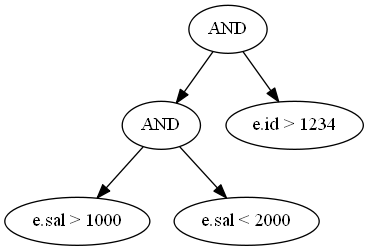
\includegraphics[scale=0.7]{Bilder/where_syntax.png}
\caption{WHERE-Bedingung in üblichen Syntaxbäumen}
\end{figure}

Der ZQL-Parser funktioniert so allerdings nicht. Wird keine spezielle Klammerung benutzt, so werden gleichrangige Operatoren nicht assoziativ geklammert, sondern befinden sich auf einer Ebene des Baumes. Somit handelt es sich nicht um einen binären Baum. 

Wir erhalten also aus obigen \verb|WHERE|-Ausdruck:
\begin{verbatim}
((e.sal > 1000) AND (e.sal < 2000) AND (e.id > 1234))
\end{verbatim}

\begin{figure}
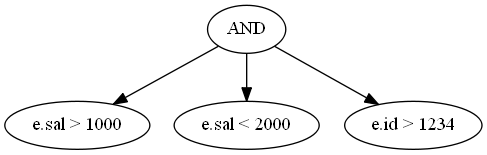
\includegraphics[scale=0.7]{Bilder/with_zql.png}
\caption{WHERE-Bedingung geparst mit ZQL}
\end{figure}
%ende baumerklaerung

So erklärt sich auch die Verwendung eines \textit{Vector} zur Speicherung der Operanden.

Die Klasse \textbf{ZConstant} dient zur Darstellung von SQL-Konstanten. Sie speichert den Wert der Konstante sowie den Typ. Als Typen kommen in Frage: \verb|NULL, NUMBER, STRING, UNKNOWN| oder \verb|COLUMNNAME|. Spaltennamen zählen hier auch zu Konstanten, da ein Spaltenname kein Operator mit Operanden ist, was einer \verb|ZExpression| entsprechen würde.

Ein Objekt der Klasse \textbf{ZGroupBy} speichert im Wesentlichen zwei Informationen. Die \verb|GROUP BY| Ausdrücke werden gespeichert in einem \textit{Vector} von Klassen, die das \verb|ZExp| Interface implementiert haben. Der optionale \verb|HAVING BY| Ausdruck wird als Objekt einer der Klassen gespeichert, welche \verb|ZExp| implementieren. Typischerweise wird das ein Objekt der Klasse \verb|ZExpression| sein.

Die Klasse \textbf{ZOrderBy} speichert einzelne Sortierkriterien. Gebündelt werden diese dann über einen \textit{Vector}. Ein Objekt der Klasse \verb|ZOrderBy| enthält einen Ausdruck vom Typ \verb|ZExp| sowie die Information ob nach dem Suchkriterium aufsteigend oder absteigend sortiert werden soll.

Letztendlich vereinigt die Klasse \textbf{ZQuery} die eben vorgestellten Klassen. Die Funktion \\\verb|getSelect()| liefert einen \textit{Vector} von \verb|ZSelectItem| zurück. Ähnlich dazu liefert die Methode \verb|getFrom()| einen \textit{Vector} von \verb|ZFromItem| zurück. Hier erkennt man schon eine Beschränkung des Parsers. Da der \verb|FROM|-Teil nur als Ansammlung von \verb|FROM|-Items abstrahiert wird, werden Joins unter \verb|FROM| nicht vom Parser erfasst. Die Methode \verb|getWhere()| liefert ein Objekt zurück, was das Interface \verb|ZExp| implementiert haben muss. Typischerweise ist dies ein Objekt der Klasse \verb|ZExpression|. Analog dazu liefert die Methode \verb|getGroupBy()| ein Objekt der Klasse \verb|ZGroupBy| zurück. Die Methode \verb|getOrderBy| liefert einen \textit{Vector} von \verb|ZOrderBy|-Objekten zurück.
Schlussendlich existiert noch eine Methode \verb|isDistinct()|, die klärt ob ein \verb|DISTINCT| verwendet wurde.

Dies sind die am häufigsten gebrauchten Klassen des ZQL-Parser. Wir wollen nun die Arbeitsweise des Parsers anhand eines Beispieles verdeutlichen. Da die \verb|SELECT|-Anfragen die wohl am häufigsten gebrauchte Form der Anfragen ist, wird sich die Erklärung der Funktionsweise des Parsers beispielhaft auf diese Art der Anfragen beziehen. Wie die anderen Statements geparst werden ist dann analog schnell zu verstehen.


Eine gewöhnliches Select-Statement wird wie folgt vom Parser zerlegt:
\begin{verbatim}
SELECT e.name, sal, dname 
FROM emp e, dept d 
WHERE e.sal > 1000 AND e.did = d.id 
ORDER BY e.sal DESC\end{verbatim}

Die ganze Anfrage wird in einem Objekt vom Typ \verb|ZQuery| eingebettet. Wir gehen nun nacheinander die Bestandteile dieses Objektes durch. 

Der \textbf{SELECT}-Teil wird durch einen \textit{Vector} dargestellt. Alle Items sind vom Typ \textit{ZSelectItem}. \verb|SelectVector = { sel1, sel2, sel3 }|.

\verb|sel1 = { [Table=e], [Column=name], [Expression=e.name], [Wildcard=false] }|

\verb|sel2 = { [Column=sal], [Expression=sal], [Wildcard=false] }|

\verb|sel3 = { [Column=dname], [Expression=dname], [Wildcard=false] }|

Auch im \verb|FROM|-Teil finden wir einen \textit{Vector}, der nun aus Objekten vom Typ \verb|ZFromItem| besteht. \verb|FromVector = { fromItem1, fromItem2 }|.

\verb|fromItem1 = { [Table=emp], [Alias=e] }|\\
\verb|fromItem2 = { [Table=dept], [Alias=d] }|

Kommen wir nun zum komplexeren Teil, dem \verb|WHERE|-Ausdruck. Da diese Struktur baumartig ist, lässt sich dies zunächst besser in einem Bild ausdrücken.

\begin{figure}[H]
\centering
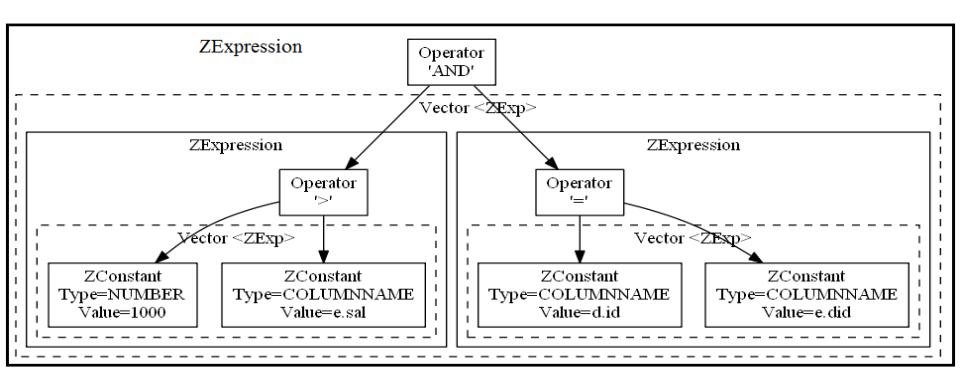
\includegraphics[scale=0.49]{Bilder/where_teil.png}
\caption{Geparster Baum der WHERE Bedingung des Beispiels}
\label{fig:parseTree}
\end{figure}

In Abbildung \ref{fig:parseTree} sieht man nun den geparsten Baum der \verb|WHERE|-Bedingung. Die gestrichelten K"asten sollen andeuten, dass es sich um den \textit{Vector} von Klassen handelt, die \verb|ZExp| implementieren, während durchgezogene Kasten konkrete Objekte sein sollen.

Der \verb|ORDER BY|-Teil wird wiederum als \textit{Vector} von \textit{ZOrderBy}-Objekten gspeichert.\\
\verb|OrderByVector = { orderBy1 }|.

\verb|orderBy1 = { [asc = false], [expression = e.sal] }|

\subsection{Grenzen des Parsers}
\label{subsec:grenzenparser}

Der Parser kann keine \verb|CREATE TABLE|-Statements parsen. Somit ist es im Rahmen dieser Arbeit notwendig, den Parser zu erweitern, damit Tabellen in eigene Datenstrukturen geparst werden können. Für die Arbeit ist es zunächst nur notwendig Name, Datentyp, Fremdschlüsselbeziehungen und NULL-Informationen der Spalten in eine interne Datenstruktur zu überführen. Dabei wird beim Typ nur zwischen Zahlen und Sonstigem (Text) unterschieden. Wir speichern außerdem, wie viele Nachkommastellen ein Attribut haben kann. Unser Programm soll in der Lage sein, einfache arithmetische Operationen durchzuführen. Dazu ist das Wissen um Datentypen der Variablen von Nöten.

Der ZQL-Parser versteht das \verb|FROM|-Statement als Liste von Relationen mit optionalen Tupelvariablen. Dadurch leiten sich mehrere Einschränkungen ab. ZQL ist dadurch nicht in der Lage \verb|JOINS| über die Schlüsselworte \\\verb#  ON [LEFT OUTER|RIGHT OUTER|INNER] JOIN# \\zu erkennen. Der Parser erkennt nur innere \verb|JOINS|, die im \verb|WHERE|-Teil formuliert worden. Der ZQL-Parser unterstützt daher auch keine Unterabfragen unter \verb|FROM|. Eine Möglichkeit diesem Problem zu begegnen ist es, solche Unterabfragen vor dem Parsen zu Entfernen und danach unverändert wieder einzufügen. Es wäre allerdings wünschenswerter wenn der ZQL-Parser erweitert würde, so dass auch ein \verb|ZQuery| als \verb|ZFromItem| benutzt werden kann.

Trotz dieser Einschränkungen sind alle Konzepte, die in dieser Arbeit vorgestellt werden einfach auf jedweden SQL-Parser übertragbar.


\subsubsection*{Beurteilung des Parsers}

Vorteile des Parsers sind seine leichte und intuitive Bedienung. Man benötigt nur wenig Einarbeitungszeit, um zu verstehen wie der Parser funktioniert und zu bedienen ist. Weiterhin positiv anzumerken ist, dass er quelloffen ist und mit einem freien Parsergenerator \cite{javacc1} entworfen ist. Dadurch ist er leicht erweiterbar.

Nachteile des Parsers sind seine schwache Dokumentation. Zur Verfügung steht lediglich ein Beispiel und die API-Beschreibung als Javadocs. Kompensiert wird diese Schwäche zwar durch die leichte Einarbeitung, weitere Mängel des Parsers findet man so aber erst in seinem Betrieb heraus. Die wohl größten Probleme hat der Parser damit, dass wichtige und handelsübliche SQL-Konstrukte nicht unterstützt werden. Die fehlende Unterstützung für Unterabfragen unter \verb|FROM| sowie das fehlende Parsen von \verb|CREATE TABLE|-Statements, schränken die Benutzbarkeit des Parsers stark ein. 

Für eine Weiterentwicklung unseres Programms bietet es sich an, den Parser von genannten Schwächen zu befreien oder zu einem Parser zu wechseln, dessen Funktionsumfang höher ist.

%TODO: CREATE TABLE

\section{JavaServer Pages}

JavaServer Pages (JSP), ist eine auf JHTML basierende Web-Programmiersprache zur dynamischen Erzeugung von HTML- oder XML-Dokumenten auf einem Webserver. Im Jahre 1999 wurden die JSP von Sun Microsystems veröffentlicht. Man kann sich die JSP als High-Level Abstraktion eines Java Servlets vorstellen. JSP werden zur Laufzeit in Servlets umgewandelt. Jedes dieser JSP-Servlets wird gecached und wiederverwendet, bis die Original-JSP verändert wurde. Ein skizzenhaftes Schema, finden wir in Abbildung \ref{fig:jsp}

\begin{figure}[h]
\begin{subfigure}[b]{.4\textwidth}
 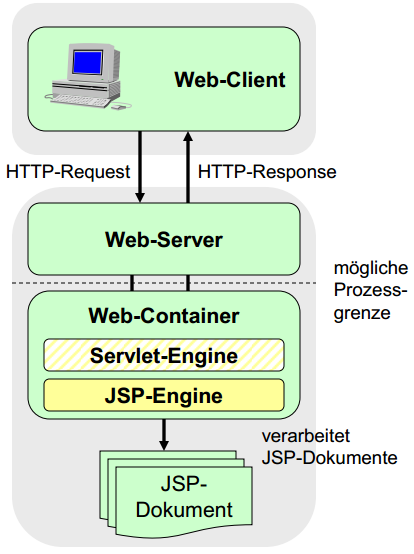
\includegraphics[scale=0.3]{Bilder/jsp.png}
 \caption{JSP-Konzep}
 \label{fig:jsp}
\end{subfigure}
\begin{subfigure}[b]{.5\textwidth}
\begin{tabular}{|l|l|}
\hline
\textbf{Objekt} & \textbf{Typ} \\\hline
request	& javax.servlet.http.HttpServletRequest \\\hline
response & javax.servlet.http.HttpServletResponse \\\hline
session & javax.servlet.http.HttpSession \\\hline
pageContext	& javax.servlet.jsp.PageContext \\\hline
application	& javax.servlet.ServletContext \\\hline
config& javax.servlet.ServletConfig \\ \hline
out	& javax.servlet.jsp.JspWriter \\\hline
exception & java.lang.Throwable \\\hline
\end{tabular}
\caption{Implizte Objekte in JSP}
\label{fig:implicitObj}
\end{subfigure}
\caption{}
\end{figure}


Man könnte die JSP als Erweiterung der Servlets ansehen, da die JSP alle Funktionen dieser übernehmen. Zusätzlich können auch eigene Tag-Libraries erstellt werden. JSP funktioniert ähnlich wie ASP oder PHP. Sowohl Java-Servlets, als auch die JSP, haben die Aufgabe die Ausführung von Javacode dem Nutzer  per HTML verfügbar zu machen. Im Gegensatz zu den Java-Servlets, die komplett aus Javacode bestehen, bestehen JSP-Dateien aus HTML mit kurzen Einschüben von Javacode. Während man also bei den Servlets HTML-Ausgaben nur innerhalb einer Funktion bewerkstelligen kann, ist es möglich bei den JSP direkt HTML auszuschreiben.

\subsection{Funktionsweise}

Wie bereits erwähnt, handelt es sich bei einer JSP-Seite um ein HTML-Dokument. Daher gibt es hier keine expliziten Funktionen oder Klassen, die die Ausgabe eines Javaprogrammes steuern. Stattdessen stehen dem Programmierer unter JSP mehrere implizite Objekte zur Verfügung, um deren Konstruktion er sich nicht kümmern muss. Eine Übersicht der impliziten Objekte finden wir in Abbildung \ref{fig:implicitObj}. Da eine JSP-Datei im eigentlichem Sinne eine (J)HTML-Seite ist, muss der Javacode abgegrenzt werden. Wir schreiben sämtlichen Javacode daher innerhalb von \verb|<% %>|. Diese Funktionieren ähnlich wie \verb|<?php ?>| in PHP.

Wir gehen nun kurz auf wesentliche implizite Objekte ein. Das Objekt \textbf{request} beinhaltet alle Funktionen und Daten, die wir benötigen um die HTTP-Anfrage zu verarbeiten. Wir haben \mbox{z. B.} Zugriff auf: Cookies, HTTP-Header, übertragene POST- oder GET-Variablen (hier Parameter genannt).

Das \textbf{response}-Objekt ist das genaue Gegenstück zum request-Objekt. Es enthält alle Informationen für die HTTP-Response und wird vor allem genutzt, um den Content-Type festzulegen und Response-Header oder Cookies zu setzen. 

Das \textbf{session}-Objekt regelt alle wichtigen Funktionen für die aktuelle Session. Wir können hier die Session-ID abfragen, sowie Objekte zur Session hinzufügen und entfernen.

Als letztes, möchten wir das \textbf{out}-Objekt erwähnen. Es repräsentiert einen BufferedWriter, genauer JSPWriter. Das Objekt kennt im Wesentlichen die Funktionen \verb|print| und \verb|println|. In PHP entspricht dies einem \verb|echo| oder \verb|print| Befehl. Der so gedruckte Text, wird zur Laufzeit in die entstehende HTML-Datei geschrieben. 

Das folgende Beispiel soll die Verwendung der impliziten Objekte verdeutlichen, ist aber, aus Platzgründen, stark vereinfacht.
\lstset{language=Java}
\begin{lstlisting}
<%@page import="java.util.Date"%>
<%@page language="java" contentType="text/html" 
		pageEncoding="UTF-8" %>
<html xmlns="http://www.w3.org/1999/xhtml">
<head><title>Datum: <% out.print(new Date()); %></title></head>
<body>Zu dieser Seite sind 
<% out.print(request.getCookies().length); %> 
Cookies gespeichert.
</body></html>
\end{lstlisting}

\section{Auflistung der Software}

Um die Programmierung nachzuvollziehen wird im Folgenden die verwendete Software aufgelistet. Wir vermerken dabei Name, Version, Kurzbeschreibung sowie die Webpräsenz der Software.

\begin{tabular}{p{9cm}r}
\textbf{Software}: ZQL-Parser & \textbf{Version}: 2011-08-26\\
\multicolumn{2}{p{1\textwidth}}{\textbf{Beschreibung}: Ein Open-Source-Parser, der mit JavaCC, einem Java-Parser-Generator, realisiert wurde. Wir haben bereits einige Schwächen bemerkt, er ist aber leicht erweiterbar, da er quelloffen ist und unter der GNU GPLv3 steht.}\\
\multicolumn{2}{l}{\textbf{URL}: \url{http://zql.sourceforge.net/}}
\end{tabular}\\

\begin{tabular}{p{9cm}r}
\textbf{Software}: Apache Tomcat & \textbf{Version}:6.0\\
\multicolumn{2}{p{1\textwidth}}{\textbf{Beschreibung}: Tomcat ist ein Webserver, der in einem Web-Container die Servlet- und die JSP-Engine bereithält. Mit ihm ist es möglich, JSP-Seiten zu betreiben.}\\
\multicolumn{2}{l}{\textbf{URL}: \url{http://tomcat.apache.org/}}
\end{tabular}\\

\begin{tabular}{p{9cm}r}
\textbf{Software}: Oracle JDK  & \textbf{Version}:1.6.0\\
\multicolumn{2}{p{1\textwidth}}{\textbf{Beschreibung}: Das Java-JDK ist notwendig um Programme zu übersetzen und auszuführen. Wir verwenden Version 1.6.0, da im universitärem Umfeld, in dessen Rahmen unser Programm entsteht, häufig noch diese Version verwendet wird. Unser Programm ist jedoch auch kompatibel zu JDK 1.7.0.}\\
\multicolumn{2}{l}{\textbf{URL}: \url{http://www.oracle.com/technetwork/java/javase/downloads/index.html}}
\end{tabular}\\

\begin{tabular}{p{9cm}r}
\textbf{Software}: JDBC-Connector für MySQL  & \textbf{Version}:5.1.25\\
\multicolumn{2}{p{1\textwidth}}{\textbf{Beschreibung}: Java Database Connectivity (JDBC) ist eine Datenbankschnittstelle der Java-Plattform, die eine einheitliche Schnittstelle zu Datenbanken verschiedener Hersteller bietet und speziell auf relationale Datenbanken ausgerichtet ist. JDBC ist in seiner Funktion als universelle Datenbankschnittstelle vergleichbar mit z. B. ODBC unter Windows oder DBI unter Perl. Zu den Aufgaben von JDBC gehört es, Datenbankverbindungen aufzubauen und zu verwalten, SQL-Anfragen an die Datenbank weiterzuleiten und die Ergebnisse in eine für Java nutzbare Form umzuwandeln und dem Programm zur Verfügung zu stellen. Für jede spezifische Datenbank sind eigene Treiber erforderlich, die die JDBC-Spezifikation implementieren. Diese Treiber werden meist vom Hersteller des Datenbank-Systems geliefert.}\\
\multicolumn{2}{l}{\textbf{URL}: \url{http://dev.mysql.com/downloads/connector/j/}}
\end{tabular}\\

\begin{tabular}{p{9cm}r}
\textbf{Software}: JDBC-Connector für PostgreSQL  & \textbf{Version}:9.2-1003\\
\multicolumn{2}{p{1\textwidth}}{\textbf{Beschreibung}: siehe JDBC-Connector für MySQL}\\
\multicolumn{2}{l}{\textbf{URL}: \url{http://jdbc.postgresql.org/download.html}}
\end{tabular}\\

\begin{tabular}{p{9cm}r}
\textbf{Software}: JDBC-Connector für Oracle Database & \textbf{Version}:-\\
\multicolumn{2}{p{1\textwidth}}{\textbf{Beschreibung}: siehe JDBC-Connector für MySQL}\\
\multicolumn{2}{l}{\textbf{URL}: \url{http://www.oracle.com/technetwork/database/features/jdbc/index-091264.html}}
\end{tabular}\\

\chapter{Theoretische Betrachtungen}
\label{chap:theorie}
Um die Frage zu beantworten wie man zwei SQL-Anfragen miteinander vergleichen kann, muss man sich die Struktur einer solchen Anfrage betrachten. Exemplarisch betrachten wir im folgenden \verb|SELECT| Anfragen. Es werden mehrere Ansätze in diesem Teil der Arbeit verfolgt, wie man die Gleichheit von zwei Anfragen zeigen kann. Offensichtlich sind zwei SQL-Anfragen semantisch äquivalent, wenn sie ebenfalls syntaktisch äquivalent sind. Interessanter sind daher Anfragen, die zunächst nicht syntaktisch deckungsgleich sind. 

Ein Ansatz besteht darin beide SQL-Anfragen einer Standardisierung zu unterziehen. Wie genau so etwas durchgeführt werden kann, wird im Folgenden noch erläutert. Dann würden wir zwei standardisierte SQL-Anfragen erhalten. Sind diese syntaktisch äquivalent, so handelt es sich um identische Anfragen. 

Mit der Standardisierung der Anfragen können wir jedoch nur ein hinreichendes Kriterium abdecken. Schaffen wir es nicht, mit Hilfe der Standardisierung zu zeigen, dass die zwei Anfragen syntaktisch gleich und damit auch semantisch äquivalent sind, so möchten wir sicher gehen, dass die Anfragen tatsächlich nicht semantisch äquivalent sind. Dazu testen wir die Anfrage gegen ein notwendiges Kriterium. Wir führen sowohl die Anfrage der Musterlösung, als auch die Anfrage des Lernenden auf einer echten Datenbank mit konkreten Daten aus. Liefern beide Anfrage unterschiedliche Ergebnistupel, so wissen wir sicher, dass unsere Anfragen nicht semantisch äquivalent sein können. 

Einen ungeklärten Fall haben wir, wenn die beiden Anfragen durch Standardisierung nicht angepasst werden konnten und die Ergebnistupel beider Anfragen auf der konkreten Datenbank identisch sind. In diesem, dritten Fall, gelingt es uns keine Aussage über die semantische Äquivalenz zu treffen. Daher ist es wünschenswert, das Auftreten dieses Falles, so gut es geht, zu minimieren.

Zu Bemerken ist hierbei, dass im folgendem Kapitel die theoretischen Grundlagen behandelt werden, die notwendig sind, um zwei SQL-Anfragen auf semantische Äquivalenz zu prüfen. Dabei werden hier insbesondere auch Ideen vorgestellt, die nicht im praktischem Teil, dem Programm, auftauchen. 

\section{Hintergrund}

Es gibt syntaktisch unterschiedliche Anfragen, die jedoch semantisch äquivalent sind. So liefern die folgenden Anfragen die gleichen Ergebnisse obwohl sie nicht syntaktisch gleich sind. Wir nehmen für das Beispiel an, dass \verb|e.enr| vom ganzzahligem Typ Integer ist.

\begin{verbatim}
SELECT * FROM emp e WHERE e.enr > 5
\end{verbatim}

\begin{verbatim}
SELECT * FROM emp e WHERE 5 < e.enr
\end{verbatim}

\begin{verbatim}
SELECT * FROM emp e WHERE e.enr >= 6
\end{verbatim}

Wie man leicht sieht, sind die Anfragen syntaktisch ähnlich und semantisch äquivalent. 

Neben solchen syntaktischen Varianten, kann es auch sein, dass unnötige Bedingungen aufgeschrieben werden, die das Ergebnis nur unnötig kompliziert machen. Eine Möglichkeit ist folgende Anfrage, in der offensichtlich die letzte Bedingung überflüssig ist.
\begin{verbatim}
SELECT * FROM emp e WHERE e.enr > 5 AND e.enr <> 2
\end{verbatim}

Unser Programm müsste nun erkennen, dass das Attribut \verb|enr| bereits beschränkt ist, und der Wert 2 nicht mehr auftreten kann. Das Programm, was zu dieser Arbeit entwickelt wird, kann mit solchen redundanten Eigenschaften nicht umgehen. Es wäre auch eher ein Problem für einen ``semantic checker'', da es hier nicht auf zwei verschiedene Anfragen ankommt. Hier ist bereits diese eine Anfrage in sich selbst zu kompliziert. Mit solchen Problemen beschäftigt sich bereits andere Lernplattformen, die wir bereits im Kapitel \ref{chap:forschung} betrachtet haben.

Weitere Probleme sind Operatoren, die sich auf andere abbilden lassen. Man kann nie wissen, in welcher Art und Weise der Lernende die Aufgabe formulieren wird. Man betrachte dazu folgende zwei Anfragen:
\begin{verbatim}
SELECT * FROM emp e WHERE e.sal BETWEEN 10 AND 200

SELECT * FROM emp e WHERE e.sal >= 10 AND e.sal <=200
\end{verbatim}

Offensichtlich sind die Anfragen äquivalent. Dies erreichen wir im Wesentlichen, indem wir bestimmte Operatoren wie \verb|BETWEEN| abschaffen und durch äquivalente Ungleichungen mit \verb|>=| und \verb|<=| ersetzen. Ähnliches gibt es für \verb|INNER JOIN| im \verb|FROM|-Teil, mit Ersetzung durch Vergleiche im \verb|WHERE|-Teil, was wir später im Detail betrachten werden.

\section{Workflow}

Im folgendem Abschnitt erläutern wir einzelne Schritte unseres Vorgehens. Dabei ist zu beachten, dass im entstehenden Programm einige Schritte ausgelassen werden oder in einer anderen Reihenfolge vorkommen. Auslassung werden entweder in diesem Kapitel oder im Kapitel \ref{chap:praxis} erläutert. Die tatsächliche Abfolge der Schritte im Programm, finden sich im ebenso im Kapitel \ref{chap:praxis}.

\subsection{Standardisierung}

Im ersten Ansatz unterziehen wir jeder Anfrage einem Standardisierungsprozess. Ziel dabei ist es, die zwei Anfragen durch legale Umformungen so anzupassen, dass sie syntaktisch äquivalent werden. Dazu beginnen wir mit dem lexikographischem Sortieren alle vorkommenden Tabellen im FROM-Teil. Anschließend erhalten diese eine automatisch generierte Tupelvariable. Diese werden in allen anderen Teilen der SQL-Anfrage ersetzt durch bereits vorhandene, oder eingeführt, falls vorher keine Tupelvariablen benutzt worden sind. Die meiste Arbeit wird dann im WHERE-Teil erledigt. 

Dort ersetzen wir syntaktische Varianten durch einheitliche Schreibweisen und entfernen syntaktische Details. Nachdem der Ausdruck des WHERE-Teils auf eine standardisierte Form (konjunktive Normalform) gebracht wurde sortieren wir den Ausdruck so, dass eine gewisse Ordnung bezüglich der Operatoren vorliegt. Weitere Anpassungen sind das Ersetzen von jedweden Unterabfragen durch äquivalente EXISTS-Unterabfragen. Im nächsten Schritt werden Verbunde (engl. Joins) kritisch untersucht und ggf. ersetzt oder vereinfacht. 

Die Operatorenvielfalt ist ein Problem, was auf zwei unterschiedliche Arten angegangen werden kann. Wir diskutieren sowohl das Hinzufügen von implizierten Formeln, als auch das Ersetzen von Formeln durch eine repräsentante Formel des gleichen Typs. Zum Abschluss werden noch GROUP BY- und ORDER BY-Ausdrücke auf ähnliche Weise angepasst.

Sind alle diese Teilschritte ausgeführt, vergleichen wir die standardisierten Anfragen auf syntaktische Gleichheit. Bei Erfolg ist klar, dass diese ebenso semantisch äquivalent sind.

%\subsection{Elementare Transformationen}

%Der zweite Ansatz ist das Anwenden von elementaren Transformationen auf einer Anfrage A um sie an eine %zweite Anfrage B anzupassen. Dabei wird immer versucht Teile der Anfrage A durch Anwendung von elementaren %Transformationen auf Teile von Anfrage B anzupassen. 

%Zunächst wird versucht den FROM-Teil von Anfrage A anzupassen, indem wir die Anordnung der Variablennamen %permutieren. Ist dies gelungen werden Aliase, die Anfrage A jetzt verwendet, in den restlichen Teilen der %Anfrage A übernommen, ähnlich wie im Ansatz >>Standardisierung<<. Im WHERE-Teil wird durch sukzessives %Backtracking versucht beide WHERE-Ausdrücke aneinander anzupassen. Ähnlich wir dann mit GROUP BY und ORDER %BY Ausdrücken vorgegangen. Konnte das Backtracking Erfolg vermelden, so wissen wir, dass beide Anfragen %semantisch äquivalent sind. 

\subsection{Test mit konkreten Daten}

Konnten wir, durch die Standardisierung beider Anfragen, keine semantische Äquivalenz feststellen, so muss dies nicht notwendig bedeuten, dass die zwei Anfragen nicht semantisch äquivalent sind. Wir prüfen diese Tatsache, indem wir die zwei Anfragen auf einer Datenbank mit einem konkreten Datenbankzustand ausführen. Wir vergleichen anschließend die Ergebnistupel beider Anfragen. Sind diese nicht identisch, so ist klar, dass wir keine äquivalenten Anfragen haben. Sind beide jedoch identisch, wissen wir nicht mit Sicherheit, ob die Anfragen äquivalent sind, oder nicht. Wir erinnern uns, dass es im Allgemeinen nicht entscheidbar ist, ob zwei SQL-Anfragen semantisch äquivalent sind. Daher ist es unvermeidbar, dass unser Programm für eine Teilmenge von SQL-Anfragen keine definitive Aussage über die semantische Äquivalenz liefern kann. Ziel ist es natürlich diese Menge so klein wie möglich zu halten. Solche Anfragen sollten außerdem dem Dozenten präsentiert werden, damit dieser entscheiden kann, ob möglicherweise eine alternative Musterlösung eingestellt werden muss.



%\begin{verbatim}
%INPUT: QUERY Q1,Q2;
%P1 = preprocessing(Q1);
%P2 = preprocessing(Q2);
%compare(P1,P2); // possible warnings can be displayed now
%ANSWER = match(Q1,Q2);
%if ANSWER yes then
%    /* If that worked, we know both solutions are the same */
%    display success
%else 
%    if do_real_db_compare(Q1,Q2) then
%        /* now we don't know if they are the same because
%         * they couldn't be matched but test on real data 
%         * showed the correct results 
%         display may be correct
%    else 
%        /* if the real data test failed we have a proof 
%         * in form of a data set, that both querys can't be the same */
%         display fail
%    endif
%endif
%output result of compare(P1,P2)
%/* The result may show the cause of a fail or a ``may be'' solution. 
% * It can provide hints so that the student can improve.
% * Even if the solution was correct i.e. it was matched with the sample solution, 
% * it may be that the students solution contained unnecassary joins, or formulas. */
%\end{verbatim}

\subsection{Preprocessing}
\label{subsec:preprocessing}

Im Abschitt >>Forschungsstand<< haben wir bereits einige Lernplattformen/ -projekte zum Thema SQL kennen gelernt. Viele dieser Plattformen möchten dem Lernenden genügend Feedback beim Lernprozess geben. Dies ist nicht nur sinnvoll, damit der Student schneller auf korrekte Lösungen stößt, sondern auch, weil die Standardhinweise eines SQL-Systems meist nur auf syntaktische Fehler hinweisen.

Da in dieser Arbeit zwei SQL-Anfragen verglichen werden sollen, können wir nicht viele Ideen der >>semantic checker<< übernehmen. Dennoch möchten wir dem Lernenden auch ein Feedback über mögliche semantische Fehler geben. Egal ob das Matchen der Musterlösung und der Lösung des Lernenden gelingt oder nicht, ein solches Feedback über semantische Fehler ist in jedem Fall hilfreich.

Dies geschieht in folgender Art und Weise. Direkt nach dem Parsen und noch bevor wir irgendwelche Anpassungen vornehmen, analysieren wir beide Anfragen und sammeln Metainformationen über diese. Nachdem wir beide Anfragen standardisiert haben, vergleichen wir die Metainformationen beider Anfragen systematisch miteinander. Fallen uns Unterschiede auf, so teilen wir dies dem Lernenden als Hinweis mit. Neben dem bloßen Vergleich von Metainformationen sind noch andere Kriterien für den Vergleich interessant. So vergleichen wir weiterhin, ob beide Anfragen die gleichen Tabellen unter \verb|FROM| ansprechen. Auch interessiert uns in diesem Zusammenhang ob Teile der SQL-Anfragen miteinander übereinstimmen. Wir prüfen also, ob \verb|SELECT|, \verb|WHERE|, \verb|FROM|, \verb|GROUP BY| und \verb|ORDER BY| der beiden Anfragen jeweils zueinander identisch sind. So können wir dem Lernenden deutlich machen, dass \mbox{z. B.} der \verb|WHERE|-Teil seiner Lösung korrekt ist, aber der \verb|SELECT|-Teil noch nicht mit dem der Musterlösung übereinstimmt.

\subsubsection*{Atomare Formeln unter WHERE / Baumtiefe}

Enthält die Anfrage des Lernenden, vor der Transformation durch unser Programm, mehr atomare Formeln als die Musterlösung, so wurden offensichtlich unnötige Formeln oder doppelte Formeln aufgeschrieben. Stellt unser Programm fest, dass beide Lösungen dennoch gleich sind, so muss dem Lernenden mitgeteilt werden, dass er Formeln eingebaut hat, welche die Lösung unnötig verkomplizieren. Dabei muss beachtet werden, dass es durch die Verwendung unterschiedlicher Normalformen in Musterlösung und Lösung des Lernenden auch zu unterschiedlicher Anzahl von atomarer Formeln geben kann.

Gleichzeitig kann die unterschiedliche Tiefe des Parserbaumes der \verb|WHERE|-Klausel auch auf redundante Formeln hinweisen, die unser Programm durch Konstanten ersetzt hat. Beispiele dafür sind arithmetisch/logische Ausdrücke, die nur Konstanten als Operanden haben und somit auswertbar und verkürzbar sind.

\subsubsection*{Existenz von Teilen der SQL-Anfrage}

Geraden wenn der Lernende eine falsche Lösung einsendet, kann es sein, dass er sogar wichtige Teile einer Anfrage nicht benutzt, die aber von der Musterlösung verwendet werden. So ist es sinnvoll zu vergleichen, ob sowohl die Musterlösung, als auch die Lösung des Studenten einen nicht leeren \verb|SELECT-, FROM-, WHERE-, GROUP BY-| und \verb|ORDER BY-|Teil hat. Unterschiede müssen dem Lernenden mitgeteilt werden. Dabei ist sowohl die Information interessant, ob ein gewisser Teil existiert, als auch die Anzahl der Attribute oder Formeln im jeweiligen Teil der Anfrage.

\subsubsection*{Anzahl von JOINs / Unterabfragen}

Sehr viele Fehler bei Anfängern finden sich im Bereich JOINs. Gerade deswegen ist es für den Lernenden interessant, ob er mehr oder weniger JOINs verwendet hat, als die Musterlösung. Im selben Atemzug sind Unterabfragen genannt, die entweder zu zaghaft oder zu häufig von Lernenden eingesetzt werden. Daher sollte auch diese Anzahl überwacht werden.

\subsubsection*{Anzahl der Operationen}

Wie im vorherigen Abschnitt bereits erklärt ist der ZQL-Parserbaum nicht binär. Dadurch kann es durch zu vorsichtige Klammersetzung passieren, dass ein Teilbaum mit zwei Ebenen entsteht, obwohl nur ein Operator beteiligt ist. Erklärt ist dies im Abschnitt \ref{subsec:funktionparser}. Wir werden uns bei der Betrachtung des \verb|WHERE|-Teils mit diesem Problem beschäftigen. Ist die Gleichheit der Lösung des Studenten mit der Musterlösung durch unser Programm gezeigt, aber aus der Lösung des Lernenden mussten mehr Klammern entfernt werden, so muss dem Studenten mitgeteilt werden, dass einige seiner Klammern unnötig waren. Dies ist allerdings eine Information, die nur als Hinweis angezeigt werden sollte.

\subsubsection*{Auflisten der gespeicherten Metainformationen}

Es folgt eine Zusammenfassung der Informationen, die wir im Zuge des Sammelns der Metainformationen speichern wollen.

\begin{itemize}
\item Anzahl der JOIN Bedingungen
	\begin{itemize}
	\item Anzahl von OUTER/ INNER Joins
	\end{itemize}
\item Anzahl atomarer Formeln im \verb|WHERE|-Teil
\item Anzahl atomarer Formeln im \verb|HAVING|-Teil
\item Anzahl Tabellen in \verb|FROM|-Teil
\item Anzahl Attribute im \verb|SELECT|-Teil 
\item Existiert ein \verb|DISTINCT|?
\item Existiert ein \verb|GROUP BY|?  
\item Existiert ein \verb|HAVING|?
\item Tiefe des Parserbaums 
\end{itemize}

Im Allgemeinen vergleichen wir jede Metainformation der Musterlösung mit der jeweiligen Information der Lösung des Lernenden. Da für eine Aufgabe mehrere Musterlösungen hinterlegt sein können, müssen wir die Lösung des Lernenden gegen jede dieser Musterlösungen prüfen. Hat also \mbox{z. B.} keine Musterlösung ein \verb|GROUP BY| dafür aber die Lösung des Lernenden, dann wird eine Meldung erzeugt. Hätte mindestens eine Musterlösung dagegen doch ein \verb|GROUP BY| erzeugen wir keine Meldung, da wir nicht wissen welcher Musterlösung sich der Lernende nähert. Die folgenden Meldungen sind Beispiele für den Vergleich der Metainformationen:

\begin{itemize}
\item ``Jede Musterlösung enthält mindestens zwei Joins, aber ihre Lösung enthält keinen Join.''
\item ``Ihre Lösung ist korrekt, allerdings enthält jede Musterlösung mindestens zwei atomare Formeln weniger.''
\item ``Ihre Lösung ist korrekt, aber keine Musterlösung enthält ein DISTINCT. Überlegen Sie, ob dies wirklich notwendig ist..'' 
\end{itemize}

Folgende zusätzliche Vergleiche führen wir nach der Standardisierung beider Anfragen durch. Dabei bezeichnen wir die Musterlösung mit ML und die Lösung des Lernenden mit LL.

\begin{itemize}
\item Stimmen \verb|SELECT|-Teil von ML und LL überein?
\item Stimmen \verb|FROM|-Teil von ML und LL überein?
\item Stimmen \verb|WHERE|-Teil von ML und LL überein?
\item Stimmen \verb|GROUP BY|-Teil von ML und LL überein?
\item Stimmen \verb|HAVING|-Teil von ML und LL überein?
\item Stimmen \verb|ORDER BY|-Teil von ML und LL überein?
\end{itemize}

Zu bemerken ist, dass die Meldungen nicht immer zielführend sind. So kann man die Benutzung eines \verb|DISTINCT| in manchen Fällen auch mit einem \verb|EXISTS| umgehen. Da wir dieses Problem in dieser Arbeit nicht behandeln muss der Dozent in solchen Fällen beide Lösungen als Musterlösung hinterlegen.

Zusammenfassend kann man Folgendes sagen: Das Preprocessing wird direkt nach dem Parsen einer SQL-Anfrage durchgeführt. Es sammelt Metainformationen über die Anfrage. Da wir zwei Anfragen vergleichen, werden diese Metainformationen einzeln für jede Anfrage gespeichert. Dann beginnen wir mit den weiteren Schritten, die im Folgenden detailliert erläutert werden.

Egal ob die Ergebnisse in diesen weiteren Schritt erfolgreich waren oder nicht, wir geben danach einen Vergleich der Metainformationen aus. Zusätzlich führen wir weitere Vergleiche mit den standardisierten Anfragen durch, welche eben bereits dokumentiert worden. Das soll dem Lernenden bei falschen Lösungen Anhaltspunkte geben, wie eine richtige Lösung aussehen könnte. Bei einer korrekten Lösung, können solche Hinweise trotzdem nützlich sein, denn die Anfrage des Lernenden kann trotz Korrektheit zu lang bzw. zu kompliziert sein. Dies würde bei einem Vergleich der gesammelten Metainformationen deutlich werden.

\section{Standardisierung von SQL-Anfragen}

Zunächst verfolgen wir den Ansatz zwei SQL-Anfragen zu vergleichen, indem wir sie standardisieren. Wir erhoffen uns durch die Standardisierung eine syntaktische Gleichheit beider Anfragen zu erreichen. Dies würde automatisch eine semantische Äquivalenz bedeuten. Die Kriterien der Standardisierung werden im Detail behandelt. Standardisiert man die Musterlösung, als auch die Lösung des Lernenden nach den gleichen Kriterien, so kann man danach durch einen einfachen Stringvergleich auf die syntaktische, und damit auch auf die semantische, Äquivalenz schließen. 

\subsection{Entfernen von syntaktischen Details}

Das Entfernen von syntaktischen Details übernimmt zu einem Teil bereits der Parser. Er entfernt unnötige Leerzeichen, Kommentare sowie unnötige Klammern. Aufgrund der Arbeitsweise des Parsers gibt es allerdings Situationen, in denen der Parser nicht alle unnötigen Klammern entfernt. Wie im Abschnitt >>Verwendeter Parser<< erläutert wurde, sind die geparsten Bäume nicht binär. Unnötige Klammerungen müssen daher eventuell nachträglich entfernt werden. Dazu stellen wir noch eine Methode vor.

Der Parser hilft allerdings dabei die SQL-Anfrage in einer Datenstruktur zu überführen, die frei von allen syntaktischen Details ist. Dazu gehören Leerzeichen, Tabs, Zeilenumbrüche und Groß-/ Kleinschreibung von Schlüsselwörtern.


\subsection{SELECT-Teil}
\label{subsec:select}

Im \verb|SELECT|-Teil ersetzen wir zunächst alle Wildcard \verb|*| vorkommen mit den entsprechenden Spaltennamen, egal ob diese mit oder ohne Tupelvariable stehen. 
Haben wir dabei nur das Wildcard \verb|*| ohne Tupelvariable, so müssen wir auf die Reihenfolge der Relationen unter \verb|FROM| beachten. Wurde in der Aufgabenstellung vermerkt, dass die Reihenfolge der Spalten keine Rolle spielt, so können wir diese jetzt lexikographisch sortieren. 

Bei explizit angegebenen Spaltenüberschriften hat der Parser das Wort \verb|AS| entfernt und damit ist keine Anpassung notwendig. Ist in der Aufgabenstellung vermerkt, dass Spaltenüberschriften nicht von Bedeutung sind, so entfernen wir in diesem Abschnitt alle Spaltenüberschriften. Hat der Nutzer als eine explizite Spaltenüberschrift gewählt, welche identisch mit der impliziten Spaltenüberschrift ist, so wird diese dennoch abgespeichert. In diesem Fall entfernen wir die Spaltenüberschrift, auch wenn sie in Groß- und Kleinschreibung nicht übereinstimmen, da diese für die Standardisierung unwichtig ist.

Als nächstes wird der \verb|FROM|-Teil bearbeitet, in dem auch künstliche Tupelvariablen eingeführt werden. Diese müssen dann auch im \verb|SELECT|-Teil eingesetzt werden.

\subsection{FROM-Teil}
\label{subsec:from}

Da wir im \verb|SELECT|-Teil jegliche Wildcards durch Spaltennamen ersetzt haben, können wir jetzt die Tabellen unter \verb|FROM| lexikographisch sortieren. Danach werden automatische Tupelvariablen erzeugt. Sind bereits Tupelvariablen vom Nutzer vergeben wurden, so werden diese ebenfalls durch die automatischen ersetzt. Eine Hashtabelle speichert frühere Zuweisungen, damit im \verb|SELECT|-, \verb|WHERE|-, \verb|GROUP BY|- und \verb|ORDER BY|-Teil die Tupelvariablen ebenfalls korrekt ersetzt werden.

Hatten die vorkommenden Tabellen im \verb|FROM|-Teil keine Tupelvariablen, so werden künstliche eingeführt.

\begin{figure}[H]
Eingabe: \\\verb|SELECT e.id, e.name, d.region FROM emp e, dep d WHERE e.depid = d.id|\\

Anpassung: \\\verb|SELECT a2.id, a2.name, a1.region FROM dep a1, emp a2 WHERE a2.depid = a1.id|\\
\caption{Beispiel: Umwandlung des FROM-Teils einer SQL-Anfrage}
\end{figure}

Wir führen auch künstliche Tupelvariablen für Unterabfragen unter \verb|WHERE| ein. Für Unterabfragen der gleichen Ebene werden dabei möglicherweise gleiche Tupelvariablen benutzt, da diese Unterabfragen disjunkt sind. Für verschachtelte Unteranfragen, werden die Tupelvariablen in natürlicher Weise iteriert. Das folgende Beispiel verdeutlicht dies:

\begin{verbatim}
Original:
SELECT ename FROM emp 
WHERE sal > (SELECT AVG(sal) FROM emp) 
AND empno > (SELECT AVG(empno) FROM emp)

Angepasste Anfrage:
SELECT a1.ename from emp a1 
WHERE a1.sal > (SELECT AVG(a2.sal) FROM emp a2)
AND a1.empno > (SELECT AVG(a2.empno) FROM emp a2)
\end{verbatim}

\subsection{WHERE-Teil}
\label{subsec:where}

Es ist wünschenswert eine Normalform des \verb|WHERE|-Teils zu erreichen, da dies die Übersichtlichkeit steigert und eine wichtige Voraussetzung zum Bearbeiten ist. Wir möchten den \verb|WHERE|-Teil in eine konjunktive Normalform (KNF) überführen, da Anwender oft SQL-Anfragen formulieren, die konjunktiv einzelne Bedingungen verknüpfen. 

\subsubsection{Entfernung unnötiger Klammerungen}
\label{subsubsec:opcomp}

Ein Ausdruck \verb|((a > 5)  AND ((b > 5) AND (c > 5)))| enthält unnötige Klammern, da der Operator \verb|AND| als Operand von einem weiteren \verb|AND| vorkommt. Folgender Ausdruck ist äquivalent: \verb|((a > 5) AND (b > 5) AND (c > 5))|. Diese spezielle Form der Klammerung entsteht aus der Tatsache, dass der ZQL-Parserbaum nicht binär ist und beide eben genannten Beispiele nicht den gleichen Baum beschreiben. Als ersten Schritt in Richtung KNF möchten wir solche unnötigen Klammern entfernen. 

Es ist daher wünschenswert, wenn ein Operator $op1$ einen Operanden als Kindknoten besitzt, der wiederum $op1$ repräsentiert, den Kindknoten zu eliminieren. Alle Kinder vom eliminierten Kindknoten hängen wir nun an den verbleibenden Operatorknoten $op1$ an. Damit hätte man den Ausdruck vereinfacht, da die assoziative Klammerung wegfällt. Dieses Vorgehen funktioniert nur bei assoziativen, nicht arithmetischen Operatoren, dies ist darin begründet, dass der Parser arithmetische Operatoren in einem binären Baum parst und linksassoziativ klammert. Wir nennen dieses Vorgehen im Folgenden \textbf{Operatorkompression}. Verbildlicht wird dieser Vorgang in Abbildung \ref{fig:opcomp}. $T(x), T(y)$ und $T(z)$ stellen dabei beliebige Teilbäume dar.

\begin{figure}[H]
\centering
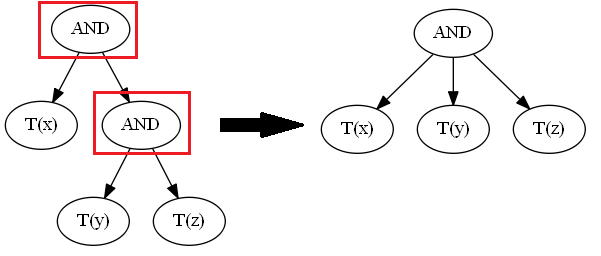
\includegraphics[scale=0.4]{Bilder/op_comp.png}
\caption{Operatorkompression}
\label{fig:opcomp}
\end{figure}

Gegeben sei der ZQL-Parsebaum $B=(V,E)$. Es sei $children(v) = \{ w : w\in V \wedge (v,w)\in E\}$, also die Menge aller Kindknoten von $v$. Gilt $v\in V$ und sei $v$ ein innerer Knoten, dann muss $v$ einen Operator repräsentieren, den wir mit $\mathit{operator}(v)$ erhalten. Gibt es einen Knoten $w\in children(v)$ mit $\mathit{operator}(v)=\mathit{operator}(w)$, so wird Knoten $w$ eliminiert und alle Kindknoten von $w$ werden zu Kindknoten von $v$, also $children(v) := children(v) \cup children(w) \setminus \{w\}$ und $E=E\backslash \{ (w,x) : x\in children(w)\} \cup \{(v,x) x\in children(w)\}$ und $V=V\backslash \{w\}$.

Im Sinne des Vergleiches der Komplexität der Musterlösung mit der Komplexität der Lösung des Lernenden ist es sinnvoll zu speichern, ob und wie oft eine solche Operatorkompression durchgeführt werden musste.

\subsubsection{NOT auflösen}

Im nächsten Schritt möchten wir auftretende \verb|NOT|-Operatoren entfernen. Dies geschieht, indem der Operator \verb|NOT| im Parserbaum nach unten geschoben wird. Dabei werden die \textit{DE MORGAN}-Regeln angewendet. 

\begin{tabular}{ll}
Eingabe: & Umwandlung Teil 1:\\
\verb|not ((a > 5)  and ((b > 5) or (c > 5)))| & \verb|(not(a > 5) or not((b > 5) or (c > 5)))|\\
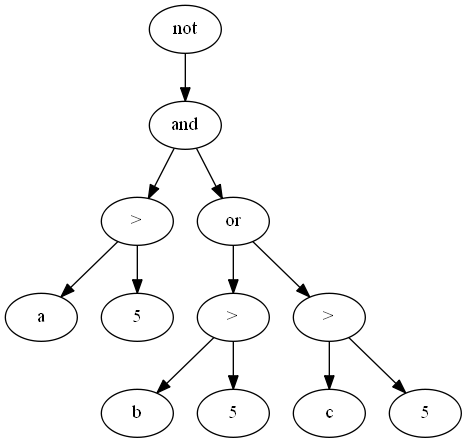
\includegraphics[scale=0.5]{Bilder/not_graph1.png} & 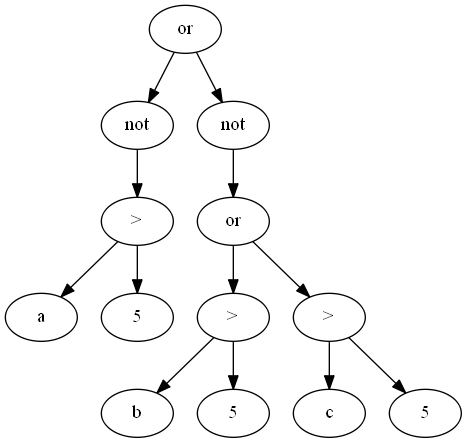
\includegraphics[scale=0.5]{Bilder/not_graph2.png}\\
\end{tabular}

\begin{tabular}{ll}
Umwandlung Teil 2: & Umwandlung Teil 3:\\
\verb|((a <= 5) or (not(b > 5) and not(c > 5)))| & \verb|((a <= 5) or ((b <= 5) and (c <= 5)))|\\
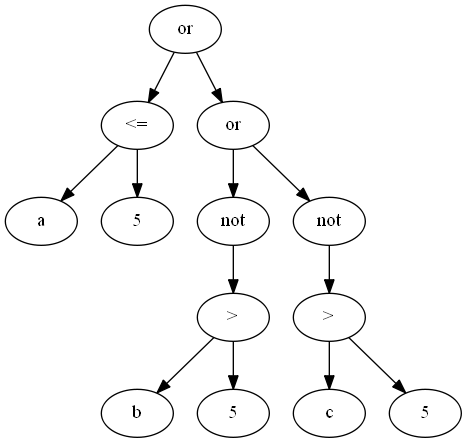
\includegraphics[scale=0.5]{Bilder/not_graph3.png} & 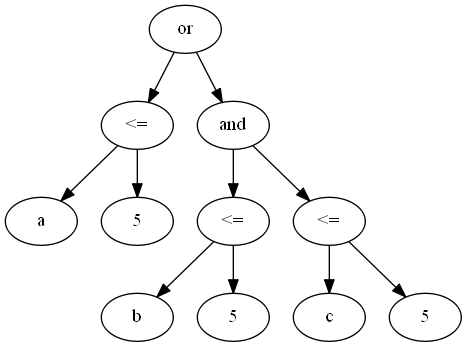
\includegraphics[scale=0.5]{Bilder/not_graph4.png}\\
\end{tabular}


\subsubsection{Anwenden des Distributivgesetzes}

Im letzten Schritt haben wir die Formel \verb|((a <= 5) or ((b <= 5) and (c <= 5)))| erhalten. Durch Anwenden des Distributivgesetzes können wir diese Formel im letzten Schritt umformen zu: \verb|((a <= 5) or (b <= 5)) and ((a <= 5) or (c <= 5))|

Im Allgemeinen durchsuchen wir den Parserbaum auf Konstellationen, in denen ein Knoten mit dem Operator \verb|OR|, Elternknoten von einem \verb|AND|-Knoten ist. Dann müssen wir auf diesen Teilbaum das Distributivgesetz anwenden. Wir wiederholen diesen Vorgang, bis kein \verb|OR|-Knoten mehr Vorfahr eines \verb|AND|-Knotens ist.

\subsection{Ersetzung von syntaktischen Varianten}

Um eine Anfrage zu standardisieren müssen wir den syntaktischen Zucker entfernen. Dies geschieht, indem man nur eine syntaktische Schreibweise anerkennt und alle anderen Schreibweisen in die zulässige umgewandelt. 

Mit dem Operator \verb|BETWEEN| testen wir ob ein gegebener Ausdruck zwischen zwei Werten, lower und upper, befindet. Wir schreiben den Ausdruck \verb|e BETWEEN lower AND upper| äquivalent um, in dem wir nur Vergleichsoperatoren benutzten. \\Unser Ausdruck lautet dann: \verb|e >= lower AND e <= upper|.

Der Operator \verb|IN| prüft, ob ein gegebener Ausdruck einem bestimmten Wert aus einer Liste zugewiesen ist. Die Liste kann dabei als Unterabfrage oder als Liste von Konstanten beschrieben werden. Handelt es sich um eine Liste von Konstanten, so können wir \\\verb|e IN (const1, const2, ..., constn)| ersetzen, in dem wir prüfen ob \verb|e| einen der konstanten Werte annimmt. Wir verknüpfen also $n$ Vergleiche disjunktiv miteinander. Wir erhalten dadurch: \verb|e = const1 OR e = const2 OR ... OR e = constn|.

Ähnlich dazu verhält sich der Operator \verb|ALL|. Er tritt in folgender Form auf:\\
\verb|operand comparison_operator ALL (subquery)|. Dabei kann \verb|subquery| auch eine Liste von Konstanten sein. Es wird in jedem Fall geprüft ob der Operand und jedes der Listenelemente in der Vergleichsrelation enthalten ist. Haben wir als \verb|subquery| eine Liste von Konstanten, so ist dies äquivalent mit dem paarweisen Vergleich von \verb|operand| und jedem Listenelement. Diese $n$ Vergleiche werden dann konjunktiv verknüpft, also: \\
\verb|operand operator elem1 AND ... AND operand operator elemn|. 
Diese syntaktische Anpassung ist nicht im Programm enthalten, da der ZQL-Parser keine Listen unter \verb|ALL| versteht.

Der Operator \verb|ANY| ist beinahe äquivalent zu \verb|ALL| mit dem Unterschied, dass die entstandene Liste der Vergleiche nicht konjunktiv, sondern disjunktiv verknüpft wird.

Befindet sich im \verb|WHERE|-Teil eine \verb|EXISTS|-Unterabfrage, so können wir den \verb|SELECT|-Teil dieser Unterabfrage vereinfachen. Da wir nur wissen wollen ob es Ergebnistupel aus der Unterabfrage gibt, benötigen wir keine konkreten Spalten aus der Unterabfrage. Daher ersetzen wir den \verb|SELECT|-Teil von \verb|EXISTS|-Unterabfragen zu:\verb|SELECT 1|. Ein Beispiel dieser Umwandlung ist in Abbildung \ref{fig:exists_ex1} zu sehen.

\begin{figure}[H]
\begin{verbatim}
SELECT e.sal FROM emp e WHERE EXISTS (
    SELECT expression FROM dept d 
    WHERE e.deptno = d.deptno )
    
SELECT e.sal FROM emp e WHERE EXISTS (
    SELECT 1 FROM dept d 
    WHERE e.deptno = d.deptno )
\end{verbatim}
\caption{Umwandlung des SELECT-Teils einer EXISTS-Unterabfrage}
\label{fig:exists_ex1}
\end{figure}


%\begin{figure}[H]
%\begin{tabular}{ccl}
%\verb|A BETWEEN B AND C| & $\to$  & \verb|A >= B AND A <= C|\\
%\verb|SELECT ALL| & $\to$ & \verb|SELECT|\\
%\verb|ORDER BY VAR ASC| &  $\to$ & \verb|ORDER BY VAR|\\
%\verb|A IN ('X', 'Y', 'Z')| & $\to$ & \verb|A = 'X' OR A = 'Y' OR A='Z'|\\
%\verb|EXISTS (SELECT A,B,C ...)| & $\to$ & \verb|EXISTS (SELECT 1 ...)|\\
%\end{tabular}
%\caption{Entfernen von syntaktischen Varianten}
%\end{figure}

\subsubsection*{Unteranfragen}

Es ist bekannt, dass sämtliche Typen von Unteranfragen eliminiert oder durch \verb|EXISTS|-Anfragen ersetzt werden können. Streng genommen handelt es sich hier zwar um mehr als nur eine syntaktische Variante, aber dennoch wollen wir das Ersetzen von Unteranfragen in diesem Abschnitt betrachten.

Wir behandeln in diesem Abschnitt nur echte Unterabfragen, das heißt die Unterabfrage darf keine Liste von Konstanten sein. Ist die Unterabfrage eine Liste, \mbox{z. B.} bei \verb|ALL, ANY| oder \verb|IN| gehen wir vor, wie im vorherigen Abschnitt beschrieben.

Für alle folgenden Umwandlungen müssen bestimmte Voraussetzungen erfüllt werden. Diese besprechen wir nachdem wir die Umformungen besprochen haben. Alles diese Umformungen sind auch in unserem Programm zu finden.

\subsubsection*{ALL-Unterabfragen}

\verb|ALL|-Unterabfragen haben immer das Muster: \verb|operand comparison_operator ALL (subquery)|. Dabei handelt es sich bei einem \verb|comparision_operator| um einen Operator aus der Menge: \verb|{=,<>,>,<,>=,<=}|. Die Unterabfrage \verb|subquery| liefert ein Attributen. Dann wird so verfahren wie bereits im letzten Abschnitt erklärt. Unser Ziel ist es, diese Unterabfrage, wenn möglich, zu ersetzen durch eine \verb|EXISTS|-Unterabfrage. Um diese Umwandlung nachzuvollziehen, wandeln wir zunächst die Unterabfrage mit \verb|ALL| in eine Unterabfrage mit \verb|ANY| um. Dazu ersetzen wir den \verb|comparison_operator| mit seinem gegenteiligem Operator. Folgende Paare sind jeweils voneinander gegenteilige Operatoren: \verb|{ {<,>=}, {>,<=}, {=,<>} }|. Danach ersetzen wir \verb|ALL| mit \verb|ANY| und kapseln die gesamte Unterabfrage mit einem \verb|NOT|. 

%\begin{figure}
\begin{lstlisting}[mathescape]
WHERE $t_1$ comparison_operator ALL (
	SELECT $t_2$
	FROM $R_1$ $X_1$, ..., $R_n$ $X_n$
	WHERE ($\varphi$)
)

Geschrieben als ANY-Unterabfrage:
WHERE NOT( $t_1\ $opposite(comparison_operator$)$ ANY (
	SELECT $t_2$
	FROM $R_1$ $X_1$, ..., $R_n$ $X_n$
	WHERE ($\varphi$) ) 
)
\end{lstlisting}

Diese \verb|ANY|-Unterabfrage können wir nun in eine \verb|EXISTS|-Unterabfrage transformieren. Wie das genau durchgeführt wird, behandeln wir im nächsten Absatz.

%\caption{Umwandeln von \verb|ALL|- in \verb|ANY|-Unterabfrage}
%\label{fig:all_ex2}
%\end{figure}

\subsubsection*{ANY/ SOME-Unterabfragen}

Da \verb|SOME| und \verb|ANY| äquivalente und synonyme Schlüsselworte sind, ersetzen wir das Schlüsselwort \verb|SOME| durch \verb|ANY|. Damit reicht es im Folgenden nur \verb|ANY|-Unterabfragen zu betrachten. Eine solche Unterabfrage kann in eine \verb|EXISTS|-Unterabfrage umgewandelt werden. Dazu verknüpfen wir den Vergleichsoperator mitsamt linken Operanden konjunktiv mit dem \verb|WHERE|-Teil der Unterabfrage. Als rechten Operanden wählen wir das Attribut, welches sich im \verb|SELECT|-Teil der Unterabfrage befindet. Die Umwandlung findet also nach folgendem Muster statt:

\begin{lstlisting}[mathescape]
WHERE $t_1\ $comparison_operator ANY (
	SELECT $t_2$
	FROM $R_1$ $X_1$, ..., $R_n$ $X_n$
	WHERE ($\varphi$) 
) 

Geschrieben als EXISTS-Unterabfrage:
WHERE EXISTS( 
	SELECT 1
	FROM $R_1$ $X_1$, ..., $R_n$ $X_n$
	WHERE ($\varphi$ 
	AND $t_1$ comparison_operator $t_2$ )
)
\end{lstlisting}

\subsubsection*{IN-Unterabfragen}

Das Schlüsselwort \verb|IN| ist lediglich ein Synonym für \verb|= ANY|. Diese Unterabfragen sind daher ein Spezialfall der, bereits betrachteten, \verb|ANY|-Unterabfragen.

\subsubsection*{Voraussetzungen}

Alle, eben genannten, Umwandlungen können nur durchgeführt werden, wenn bestimmte Bedingungen erfüllt sind.

\begin{enumerate}
\item Alle Tupelvariablen, die in $t_1$ vorkommen, müssen sich unterscheiden von allen $X_i$. Erreicht wird dies ggf. durch Umbenennung der $X_i$, da diese nicht für die eigentliche (Ober)anfrage wichtig sind.\\
\textbf{Unser Programm:} Wie bereits deutlich gemacht, erstellen wir unsere Tupelvariablen iterativ. In einer Unterabfrage wird die Iteration fortgeführt. Daher ist es nicht möglich, dass Tupelvariablen aus $t_1$ gleich sind mit einer $X_i$.
\item Wenn $t_1$ Attributreferenzen $A$ ohne Tupelvariable enthält, dann dürfen die $R_i$ kein Attribut $A$ haben. Erreicht wird dies, indem ggf. die Tupelvariable eingeführt wird.\\
\textbf{Unser Programm:} Wir erstellen für jede Attributreferenz eine Tupelvariable und erfüllen daher auch die Bedingung 2.
\item Die Unteranfrage für $t_2$ darf keine Nullwerte liefern, wenn die Unterabfrage negiert ist. \\
\textbf{Unser Programm:} Behandeln wir eine nicht-negierte Unterabfrage, können wir diesen Punkt ignorieren. Haben wir aber eine negierte Unterabfrage, dann prüfen wir ob die Unterabfrage Spalten liefert, die nach Definition \verb|NULL| sein könnten. Ist dies der Fall, gehen wir vereinfacht davon aus und passen die Unterabfrage nicht an.
\end{enumerate}

\subsubsection{Andere Unteranfragen}

Ungewöhnlichere Unterabfragen, wie \mbox{z. B.} Unterabfragen unter \verb|FROM|, werden hier nicht betrachtet. Im Allgemeinen werden solche Unterabfragen kaum gebraucht und machen die Anfrage meist nur viel komplexer als notwendig. Der vorgestellte Parser unterstützt außerdem keine Unterabfragen unter \verb|FROM|. Er versteht nur Listen von Relationen mit Tupelvariablen.

\subsection{Operatorenvielfalt}

Im folgenden Abschnitt soll geklärt werden wie mit verschiedenen Schreibweisen von ein- und demselben Ausdruck umgegangen werden soll. Betrachtet man sich \mbox{z. B.} \verb|A > 5| ist dieser Ausdruck äquivalent mit \verb|5 < A|. Wenn wir wissen, dass \verb|A| ein ganzzahlige Variable ist, dann sind auch folgende Ausdrücke äquivalent: \verb|A >= 6| sowie \verb|6 <= A|. Wir betrachten nun zwei verschiedene Ansätze, die diese Probleme lösen sollen. Der erste Ansatz beschäftigt sich damit, alle implizierten Schreibweisen mit in die Formel aufzunehmen. Damit stellt man sicher, dass sich alle korrekten Schreibweisen einer Formel in der Anfrage befinden. Der zweite Ansatz beschäftigt sich damit, nur bestimmte Schreibweisen zuzulassen und alle anderen durch die zulässigen zu ersetzen.

\subsubsection{Analyse der unterschiedlichen Operatoren}

Wir unterscheiden im wesentlichen zwei Arten von Operatoren. Zunächst haben wir Operatoren, bei denen wir die Operanden in beliebiger Reihenfolge anordnen können. Wir nennen diese Operatoren, kommutative Operatoren. Dies sind \verb|{ =, AND, OR, +, *}|. Alle anderen Operatoren sind demnach nicht kommutativ, da wir die Reihenfolge der Operanden nicht ändern können, ohne den Ausdruck zu verfälschen. Zu dieser Gruppe von Operatoren zählen \verb|{ >=, >, <, <=, -, /, }|. Eine dritte Gruppe bilden unäre Operatoren, die nur einen Operanden kennen. Diese Gruppe ist aber im Sinne der Anordnung uninteressant, da wir hier keine mehrdeutig aufgeschrieben Varianten haben.

Ziel ist es nach wie vor, eine gewisse Ordnung zu definieren, so dass nach der Standardisierung semantisch gleiche Anfragen auch syntaktisch gleich sind. Betrachten wir nun einen Ausdruck mit einem Operator $op$ und $n$ Operanden, die wir fortlaufen mit $\mathit{child_1},...,\mathit{child_i},...,\mathit{child_n}$ bezeichnen. Ist $op$ ein kommutativer Operator, so können wir die Operanden $child_i$ beliebig anordnen ohne den Sinn des Ausdrucks zu verändern. Dies tun wir, indem wir eine bestimmte Sortierreihenfolge etablieren. Diese finden wir im späteren Abschnitt \ref{subsec:sort}.

Hat eine Formel einen nicht kommutativen Operator, so ist diese Sortierung nicht möglich. In einem solchen Fall müssen wir sicherstellen, dass sowohl die Musterlösung als auch die Lösung des Lernenden, die gleiche Repräsentation der Formel enthält. Ist \verb|a| eine Variable vom Typ \verb|INT|, dann sind verschiedene Repräsentationen von: \verb|a < 5| \mbox{z. B.} \verb|5 > a, a <= 4, 4 >= a|. Wir untersuchen nun zwei Ansätze, die sich mit diesem Problem beschäftigen. Im ersten Ansatz fügen wir, zu einer Formel mit einem nicht kommutativen Operator, alle implizierten Schreibweisen hinzu. Ein Beispiel dafür ist in Abbildung \ref{fig:sampleadd} zu sehen. Im zweiten Ansatz analysieren wir die Formel mit dem nicht kommutativen Operator und wählen eine bestimmte Repräsentation dieser Formel. Dadurch ist sichergestellt, dass sich in allen standardisierten SQL-Anfragen nur eine bestimme Version der Formel befindet. Ein Beispiel dafür finden wir in Abbildung \ref{fig:samplerep}. Wir gehen davon aus, dass das Attribut \verb|sal| ganzzahlig ist.

\begin{figure}[H]
\centering
\begin{verbatim}
Eingabe: SELECT * FROM emp e WHERE e.sal >= 1001
Ausgabe: SELECT * FROM emp e 
         WHERE e.sal > 1000 AND 1000 < e.sal
         AND e.sal >= 1001 AND 1001 <= e.sal
\end{verbatim}
\caption{Beispiel für das Hinzufügen implizierte Formeln}
\label{fig:sampleadd}
\end{figure}

\begin{figure}[H]
\centering
\begin{verbatim}
Eingabe: SELECT * FROM emp e WHERE e.sal >= 1001
Ausgabe: SELECT * FROM emp e WHERE e.sal > 1000
\end{verbatim}
\caption{Beispiel für das Auswählen eines Repräsentanten}
\label{fig:samplerep}
\end{figure}

Haben wir weitere Formeln hinzugefügt, so müssen wir die konjunktive Normalform wiederherstellen, da wir nun \verb|AND|-Knoten hinzugefügt haben, die nicht auf der Wurzelebene sind. 

In unserem Programm verwenden wir den Ansatz: Hinzufügen von implizierten Formeln, der im Folgenden als erster Ansatz vorgestellt wird.

\subsubsection{Hinzufügen implizierter Formeln}
\label{subsubsec:implicitformulas}

Wie bereits im vorherigen Beispiel ersichtlich, sind die hinzugefügten Formeln redundant und tragen nicht effizient zur Beschleunigung der Anfrage bei. Es soll hier lediglich sichergestellt werden, dass alle möglichen äquivalenten Formeln auftreten, da wir nicht wissen, was der Lernende für einen Repräsentanten der Formeln wählen wird. Weiterhin muss bemerkt werden, dass dadurch die gesamte SQL-Anfrage enorm aufgebläht wird. Es ist daher unbedingt notwendig, die Originalanfrage zu speichern. Weiterhin muss das Programm eine Verbindung zwischen den Formeln der Originalanfrage und den Formeln der veränderten, aufgeblähten Anfrage herstellen. Dem Lernenden soll in einem Feedback nur Fehler in der Originalanfrage aufgezeigt werden. Da intern aber mit der aufgeblähten Anfrage gearbeitet wird, muss beim Auftreten eines Fehlers oder Hinweises nachgeschlagen werden, von welchem Teil der Originalanfrage der Teil entstammt, der jetzt den Fehler auslöst.

Im Folgenden listen wir Mengen $M_i$ von Ausdrücken. Finden wir in der zu bearbeitenden SQL-Anfrage eine Formel $f$, die auf einen Ausdruck $a\in M_i$ passt, dann verknüpfen wir alle Ausdrücke $\{b : b\in M_i \wedge b \neq a\}$ konjunktiv mit $f$. Dabei sind alle Variablennamen $A,B,C$ keine (komplexen) Ausdrücke. Es handelt sich also jeweils um Blattknoten im Parserbaum. Ferner bezeichnen wir $X,Y$ als numerische Konstanten. Wir setzen dabei voraus, dass eine Vorauswertung von arithmetischen Ausdrücken stattgefunden hat. Damit können wir auch sicher sein, dass in $M_2$ keine Division durch 0 stattfindet, da $A=0$ wenn $B=0$ oder $C=0$.\\

\begin{tabular}{ll}
$M_1$ & $\{\ A=B-C\ ,\ C=B-A\ ,\ B=A+C\ \}$\\
$M_2$ & $\{\ A=B\cdot C\ ,\ C=A / B\ ,\ B=A / C\ \}$\\
$M_3$ & $\{\ A>B-C\ ,\ C>B-A\ ,\ B<A+C\ \}$\\
$M_4$ & $\{\ A<B-C\ ,\ C<B-A\ ,\ B>A+C\ \}$\\
$M_5$ & $\{\ A>B, B<A \}$\\
$M_6$ & $\{\ A\geq B, B\leq A \}$\\
$M_7$ & $\{\ A>X, A\geq X+\mathit{adjust}(A) \}$\\
$M_8$ & $\{\ A<X, A\leq X-\mathit{adjust}(A) \}$\\

\end{tabular}

Beim Vergleich mit $>$ und $<$ ist es wichtig zu wissen, wie viele Nachkommastellen die numerischen Variablen $A$ und $B$ besitzen. Es sei $\mathit{places}(A)$ die Anzahl der Nachkommastellen der Zahl $A$. Dann bezeichnen wir mit $\mathit{adjust}(A) = 1 / (10^{\mathit{places}(A)})$, einen angepassten Wert, der sich nach der Stelligkeit der Variable A richtet.

Betrachten wir als Beispiel ein Attribut \verb|salary|, welches als \verb|NUMERIC(4,2)| definiert ist. Wir wissen also, dass \verb|salary| zwei Nachkommastellen hat. Betrachten wir nun die Aussage \verb|salary >= 5|.
Wir haben auf einer Seite eine Variable (\verb|salary|) und auf der anderen Seite eine numerische Konstante (\verb|5|). Dieses Muster passt also auf $M_7$ und auf $M_6$. In $M_7$ heißt es $A\geq X+\mathit{adjust}(A)$. Bezogen auf unser Beispiel ist \verb|A=salary| und \verb|x+adjust(salary)=5|. Wir berechnen also: 
$$\mathit{adjust}(\mathit{salary}) = 1 / (10^{2}) = 1/100 = 0,01$$
Wir erhalten also \verb|x=4,99|, weil \verb|x+0,01=5|. Somit ergänzen wir unsere Ausgangsformel \verb|salary >= 5| konjunktiv mit \verb|salary > 4,99|. Weiterhin muss jetzt wegen $M_6$, \verb|5 <= salary|, und wegen $M_5$, \verb|4,99 < salary|, hinzugefügt werden.

Finden wir Ausdrücke mit $>,<,\leq,\geq$, welche als Argumente Variablen oder Konstanten haben, so unterscheiden wir also grundsätzlich drei Fälle.

Fall 1 $(M_5,M_6)$: Beide Operanden sind Variablen. In diesem Fall ergänzen wir nur den jeweils symmetrischen Operator. Da beide Operanden Variablen sind, macht es weniger Sinn jeweils $\leq,\geq$ oder $<,>$ zu ersetzen, da normalerweise ein künstliches hinzufügen eines Summanden auf einer Seite, die Anfrage unnatürlich aussehen lässt. Es ist aber auch kein Problem diese Ersetzungen dennoch durchzuführen, wenn beide Operanden Variablen sind. Die Anfrage wird dann natürlich noch weiter künstlich aufgebläht.

Fall 2 $(M_7,M_8)$: Einer der beiden Operanden ist eine numerische Konstante und der andere ist eine Variable. In diesem Fall fügen wir alle implizierten Gleichungen hinzu, also insbesondere die Operatoren $\leq,\geq,<,>$. Zu beachten ist hier, dass nicht nur Gleichungen der Form $A>X$ dazu führen, dass alle Ausdrücke von $M_7$ hinzugefügt werden. Auch wenn eine Gleichung der Form $Var1\geq 5.2$ auftaucht, werden Ersetzungen durchgeführt. Diese Gleichung passt auf das Muster $A\geq X+\mathit{adjust}(A)$. Angenommen $Var1$ hat maximal eine Nachkommastelle, so würden dann folgende Gleichungen impliziert werden: $\{\ Var1>5.1\ ,\ 5.1<Var1\ ,\ 5.2 \leq Var1\ \}$.

Fall 3: Beide Operanden sind numerische Konstanten. In dem Fall wird die logische Aussage ausgewertet. Wir verfahren dann wie in einer aussagenlogischen Formel gemäß den Gesetzen: 
\begin{center}
\begin{tabular}{lclcllclcl}
$(1)\,true $ & $\wedge$ & $ f$ & $\equiv$ & $ f$ & $(2)\,true $ & $\vee$ & $ f$ & $\equiv$ & $true$\\
$(3)\,false $ & $\wedge$ & $ f$ & $\equiv$ & $false$ & $(4)\,false $ & $\vee$ & $ f$ & $\equiv$ & $f$\\
\end{tabular}
\end{center}

Wir können diese ersetzten Werte in SQL allerdings nicht verwenden, da im Standard keine Unterstützung für konstante Wahrheitswerte existiert. Dennoch ist ZQL in der Lage diese Werte zu akzeptieren. Wir können damit eine BOTTOM-UP Auswertung von konstanten Ausdrücken realisieren. Kommt dabei heraus, dass der komplette \verb|WHERE|-Teil aus \verb|false| besteht, so muss dem Nutzer eine Meldung angezeigt werden, dass seine SQL-Anfrage stets die leere Menge liefert.

In einem anschließenden Schritt werden arithmetisch/logische Ausdrücke ausgewertet und durch ihre Ergebnis ersetzt. Dieser Schritt muss BOTTOM-UP geschehen, damit man auch mehrere Ersetzungen nach oben, im Parserbaum, weiterreicht. Haben wir am Ende einen SQL-Ausdruck dessen \verb|WHERE|-Teil aus \verb|false| besteht, dann haben wir eine Anfrage gefunden, die immer das leere Ergebnis liefern wird. In diesem Fall müssen wir natürlich eine Fehlermeldung ausgeben.

Sollten wir durch das Hinzufügen implizierter Formeln jetzt einige Formeln doppelt in unserer Anfrage haben, so werden diese bei der Sortierung entfernt.

\subsubsection{Beschränkung der Operatorenvielfalt}

Ein weiterer Ansatz das Problem der äquivalenten Formeln anzugehen, ist es bestimmte Operatoren zu >>verbieten<<. Das soll bedeuten, dass wir verbotene Operatoren definieren, welche am Ende der Umwandlungen nicht mehr in der SQL-Anfrage vorkommen dürfen. Dies wird erreicht, indem wir jeden verbotenen Operator umwandeln in einen zugehörigen, nicht-verbotenen Operator. Das Prinzip ähnelt dem eben Vorgestellten. Wir betrachten wieder die Mengen $M_i$. Des Weiteren hat jede Menge $M_i$ einen Repräsentanten $r(M_i)$. Finden wir nun in der zu bearbeitenden Anfrage eine Formel $f$, die auf eine der Ausdrücke $a\in M_i$ passt, so ersetzen wir $f$ mit $r(M_i)$. Folgende Tabelle soll die Mengen und deren Repräsentanten beschreiben.

Im Folgenden sind alle Variablennamen $A,B,C$ keine (komplexe) Ausrücke. Es handelt sich also jeweils um Blattknoten im Parserbaum. Ferner bezeichnen wir $X,Y$ als numerische Konstanten. Wir setzen dabei voraus, dass eine Vorauswertung von arithmetischen Ausdrücken stattgefunden hat. Damit können wir auch sicher sein, dass in $M_2$ keine Division durch 0 stattfindet, da $A=0$ wenn $B=0$ oder $C=0$.\\

\begin{tabular}{lll}
$i$ & $M_i$ & $r(M_i)$ \\
$1$ & $\{\ A=B-C\ ,\ C=B-A\ ,\ B=A+C\ \}$ & $B=A+C$\\
$2$ & $\{\ A=B\cdot C\ ,\ C=A / B\ ,\ B=A / C\ \}$ & $A=B\cdot C$\\
$4$ & $\{\ A>B-C\ ,\ C>B-A\ ,\ B<A+C\ \}$ & $A>B-C$ \\
$5$ & $\{\ A<B-C\ ,\ C<B-A\ ,\ B>A+C\ \}$ & $A<B-C$\\
$6$ & $\{\ A>B, B<A \}$ & $A>B$\\
$7$ & $\{\ A\geq B, B\leq A \}$ & $A\geq B$\\
$8$ & $\{\ A>X\ ,\ X<A,A\geq X+\mathit{adjust}(X)\ ,\ X\leq A - \mathit{adjust}(X)\ \}$ & $A>X$\\
\end{tabular}

Ein Beispiel soll die Prozedur verdeutlichen.\\

Es sei unsere Ausgangsanfrage: \begin{verbatim}SELECT * FROM testtable WHERE X = 6 - Y\end{verbatim}

Die Formel $X=6-Y$ finden wir in $M_1$ in Form von $A=B-C$. Wir ersetzen nun also $X=6-Y$ mit dem Repräsentanten von $M_1$, und wir bekommen: \begin{verbatim}SELECT * FROM testtable WHERE 6 = X + Y\end{verbatim}

Ein Problem bei der Verwendung von Repräsentanten durch Einschränkung der Operatorenvielfalt ist, dass es zu überlappenden Mengen kommen kann. Damit ist gemeint, dass ein Ausdruck auf mindestens zwei Mengen $M_i$ und $M_j$ mit $i\neq j$ passt. In einem solchen Fall müssen die Mengen $M_i$ und $M_j$ genauestens untersucht werden. Im Normalfall ist dann eine Verschmelzung von $M_i$ und $M_j$ möglich, da diese Äquivalenzklassen beschreiben und ein Element in nur genau einer Äquivalenzklasse vorhanden sein kann.

\subsubsection{Einschränkungen bei arithmetischen Ausdrücken}
\label{subsubsec:arithmetic}

Bevor wir zur Diskussion beider Ansätze kommen, müssen wir noch erklären, was die beiden Ansätze bisher nicht leisten können. Für beide Ansätze haben wir angenommen, dass arithmetische Ausdrücke maximal aus zwei Operanden auf der komplexen Seite bestehen. Natürlich können in der Praxis auch komplexere Ausdrücke auftauchen. Diese Arbeit aber, entsteht im Rahmen einer Lernplattform. In der Lehre kommt es selten vor, dass arithmetische Ausdrücke im Übermaß benutzt werden. Wenn sie auftauchen, sind sie auch meistens auf zwei Operanden beschränkt. Es ist kaum von Nöten komplexe arithmetische Ausdrücke in der SQL-Anfrage zu verwenden. Im Rahmen dieser Arbeit betrachten wir solche Ausdrücke also immer mit maximal zwei Operanden auf der komplexeren Seite. Dies begründet sich auch in der zunehmenden Schwierigkeit solche komplexen Ausdrücke zu behandeln, wie wir im Folgenden sehen werden.

Wir wollen uns dennoch mit der Frage beschäftigen: ``Wie könnte man komplexere arithmetische Ausdrücke anpassen?''. Die folgenden Ansätze sind nur theoretische Überlegungen und stellen kein vollendetes Konzept dar. Wir gehen in unserem Programm trotz der folgenden Diskussion von der Beschränktheit der arithmetischen Ausdrücke aus.

\subsubsection{Komplexere arithmetische Ausdrücke -- Standardisierung}

Zunächst betrachten wir den Standardisierungsansatz. Hier möchten wir alle implizierten Gleichungen hinzufügen, sodass wir sicher gehen können, dass alle möglichen äquivalenten Gleichungen auftauchen. Dies gestaltet sich für komplexere arithmetische Ausdrücke schwierig. Es müssen alle Gleichungen, die durch äquivalente Umformungen entstehen können, errechnet werden, um sie dann der Lösung hinzuzufügen. Letztendlich führt uns diese Problematik zur Permutation aller Operanden. Für einen solchen Ansatz müssten alle Operatoren kommutativ sein. Wir behelfen uns in diesem Fall, indem wir die Operatoren $-$ und $/$ umschreiben in $+$ und $*$. Es folgt ein Beispiel:

\begin{tabular}{lll}
$A=B+C-D-E+F$ & $\to$ & $A=B+C+(-D)+(-E)+F$\\
$A=B*C/D/E*F$ & $\to$ & $A=B*C*(1/D)*(1/E)*F$\\
\end{tabular}

Nun können wir die Reihenfolge der Operanden permutieren. Im letzten Schritt müssen wir auch jeden Operanden auf jede Seite der Gleichung bringen und wieder die Reihenfolge der Operanden permutieren. So erhalten wir alle möglichen Schreibweisen eines komplexen arithmetischen Ausdrucks. Zu beachten ist, dass auf diese Weise schnell, sehr viele Gleichungen produziert werden. Dies macht die Lösung stark unübersichtlich. Zu bemerken ist weiterhin, dass gemischte Ausdrücke bezüglich $+$ und $*$ deutlich schwerer zu behandeln sind, als solche, die nur $+$ oder $*$ enthalten.

\subsubsection{Komplexere arithmetische Ausdrücke -- Operatorenbeschränkung}

Im zweiten Ansatz gestaltet sich das Problem etwas einfacherer. Wie bereits im ersten Ansatz eliminieren wir die Operatoren $-$ und $/$. Da wir am Ende nur eine Schreibweise als zugelassen betrachten, müssen wir nun festlegen, welche Schritte an jedem Ausdruck ausgeführt werden müssen. Wir entscheiden uns für folgende Konvention: Alle Variablen werden via äquivalenten Umformungen auf die linke Seite der Gleichung gebracht und alle numerischen Konstanten werden auf die rechte Seite der Gleichung gebracht. Im nächsten Schritt entfernen wir doppelte Minus- bzw. Divisionszeichen, aus $-(-2)$ wird also $+2$ und aus $1/1/E$ wird $E$. Nun rechnen wir den Wert des arithmetischen Ausdrucks auf der rechten Seite aus, da dieser nun nur noch aus Konstanten besteht. Die Linke Seite sortieren wir lexikographisch nach Namen der Variablen. Es muss daran erinnert werden, dass diese Namen automatisch generiert worden sind, sodass sichergestellt ist, dass wir Übereinstimmungen später finden können.

Zusammenfassend kann gesagt werden, dass eine Behandlung von komplexeren arithmetischen Ausdrücken möglich, aber nicht einfach umzusetzen ist. Wir haben nur Ansätze präsentiert, die in einem ausgearbeiteten Zustand das Problem der Standardisierung solcher arithmetischen Ausdrücke lösen könnten. Denkbar wären auch andere Ansätze, wie \mbox{z. B.} mehrfaches substituieren von zwei Operanden zu einer Variablen.  Alles in allem bedarf es bei diesem Problem noch weiterer Forschung.

%genaueres Vorgehen unklar

\subsubsection{transitiv-implizierte Formeln}

Formeln können auch transitiv-impliziert sein. Steht in der Musterlösung die Formel \verb|A>B AND B>C| und der Student hat geschrieben \verb|A>B AND A>C AND B>C|, so sind beide Aussagen logisch identisch. Leider erkennt dies unser bisheriger Ansatz nicht. Um solche Formeln zu erkennen, müssen wir auch alle transitiv-implizierten Formeln hinzufügen. Dabei gibt es verschiedene Fälle. 

Existiert in der Formel nur eine Relation $R$, so wie im Beispiel eben $R=\ '>'$, dann können wir im Ansatz des Hinzufügens implizierter Formeln die transitive Hülle von $R$ berechnen und die entstandenen Paare der Ausgangsformel hinzufügen. Wollen wir keine implizierten Formeln hinzufügen, sondern nur bestimmte Schreibweisen erlauben, so können wir zunächst die transitive Hülle $R^+$ berechnen und danach eine transitive Reduktion durchführen. Zu beachten ist bei diesem Ansatz, dass es nicht für jede Relation eine eindeutige transitive Reduktion gibt. 

Komplexer wird das Problem, wenn eine Formel verschiedene Relationen enthält, wie \mbox{z. B.} \\\verb|A>B AND B=9|. Diese Formel impliziert eine weitere Formel transitiv, weil die Relationen $>$ und $=$ zueinander kompatibel sind. Inkompatible Relationen sind jeweils $>,\geq$ zu $\leq,<$. Die Relation $=$ ist zu jedweder Relation kompatibel. Haben wir also eine Mischformel mit mehreren kompatiblen Relationen, dann ordnen wir das entstehende transitive Paar der allgemeineren Relation zu. In unserem Beispiel entsteht das Paar $(A,9)$. Da $>$ allgemeiner ist als $=$ ordnen wir $(A,9)$ der Relation '$>$' zu. Auch hier können wir die implizierten Formeln der Ausgangsformel hinzufügen (Ansatz Hinzufügen der Implikationen) oder danach die transitive Reduktion berechnen, wie oben bereits erwähnt. Ein Ansatz eines Algorithmus für solche Mischformeln wäre einen Graph zu erzeugen mit Operanden als Knoten und Relation als Kantenbeschriftung. Zwei Knoten sind genau dann miteinander verbunden, wenn sie durch eine Relation $R_i$ miteinander in der Formel verknüpft sind. $R_i$ ist dann auch die Kantenbeschriftung. Wenn auf einem Pfad alle Relationen zueinander kompatibel sind, wird mit üblichen Methoden die transitive Hülle bestimmt, indem neue Kanten eingezeichnet werden. Beschriftet werden diese Kanten mit dem allgemeineren der Relationen, die auf dem Pfad liegt. So erhalten wir alle transitiv-implizierten Paare.

\subsubsection{implizierte Domänen}

Ein weiterer Problempunkt sind implizierte Domänen von Attributen. Es geht darum zu erfassen welchen Wertebereich einzelne Attribute durch die Formeln in der SQL-Anfrage zugewiesen bekommen. Dabei können semantische Widersprüche entdeckt werden, wie \mbox{z. B.} \verb|A>9 AND A<9|. Diese Widersprüche führen meist zu einer leeren Antwort des SQL-Systems. Eine Hinweis würde dem Lernenden klar machen, dass diese Bedingung wahrscheinlich nicht gewollt ist. Die Erfassung des Wertebereichs deckt aber auch weitere Einsatzgebiete ab. So können auch unnötige Bedingungen erkannt werden, wie \mbox{z. B.} \verb|A>9 AND A>5|. Die letzte Bedingung wird ja bereits durch die erste Bedingung impliziert. Unser Matching-Ansatz würde in diesem Fall die Lösungen nicht unifizieren können, obwohl sie äquivalent sind. Man könnte hier aber auch argumentieren, dass die Lösung des Lernenden unnötige Formeln enthält, die keinen Nutzen für die Anfrage haben, und damit unser System, korrekterweise, keine Übereinstimmung erkennt. Andererseits wäre es hilfreich, wenn ein vorgeschalteter Semantikprüfer solche Probleme erkennt, um entweder den Lernenden vorab ein Feedback zu geben oder, um solche unnötigen Formeln bei der Bearbeitung zu ignorieren. 

Da dieses Problem eher in den Bereich Semantikprüfer gehört wird dieses Feature nicht im Programm auftauchen. Will man dem Programm später aber semantische Prüfer vorschalten, wäre dies auf jeden Fall ein wichtiges und sinnvolles Feature.

\subsubsection{Diskussion der beiden Ansätze}

Ein wesentlicher Punkt beim Vergleich beider Ansätze ist der Aufwand bzw. die Laufzeit. 

Betrachten wir zunächst den Ansatz des Hinzufügens von implizierten Formeln. Wir bezeichnen mit $length = \sum_{i=0}^n \vert M_i\vert$ die Gesamtanzahl aller Formeln über allen Mengen. Wir müssen in einer Tiefensuche jede Formel betrachten und mit allen Mengen $M_i$ mit $i\in \{1,2,...,n\}$ abarbeiten. Finden wir in einer Menge ein Muster wieder, so wird unsere Formel künstlich aufgebläht. Wir haben also für das Suchen eine maximale Laufzeit von $\mathcal{O}(\mathit{\vert Formeln\vert \cdot length})$. Das Einfügen der Formeln geschieht in konstanter Zeit $\mathcal{O}(k)$ mit $k= \max_{i\in [1,n]\cap \mathbb{N}} \vert M_i\vert$.

Beim anderen Ansatz werden bestimmte Operatoren verboten. Wir realisieren dieses Verbot wieder über eine Suche. Es muss auch hier jede Formel auf ein Muster in $M_i$ untersucht werden. Wir benötigen für das Suchen in diesem Ansatz also genau so viel Zeit, wie im ersten Ansatz. Auch das Ersetzen der Formeln hat keine Zeitersparnis gegenüber einem Hinzufügen von weiteren Formeln. Es muss bemerkt werden, dass in diesem Fall die Originalformel nicht weiter aufgebläht wird.

Da sich die Laufzeiten der beiden Varianten nicht unterscheiden, müssen andere Kriterien zum Vergleich herangezogen werden. Wichtig für Software ist nicht ausschließlich die Laufzeit, sondern auch die Wartbarkeit. Besonders bei Projekten, die im Rahmen einer Masterarbeit entstehen, ist es wahrscheinlich, dass der Autor sich später nicht mehr um das Projekt kümmern kann. Daher sollte man sich bei den hier vorliegenden Ansätzen fragen, welcher leichter wartbar und erweiterbar ist.

Muss das Programm erweitert werden und wir möchten den Ansatz des Hinzufügen implizierter Gleichungen verwenden, so muss lediglich eine weitere Menge $M_k$ erstellt werden. Der Algorithmus sucht automatisch, dann auch in dieser neuen Menge nach Mustern und würde alle anderen Elemente dieser Menge konjunktiv-verknüpft zur Formel hinzufügen. 

Bei der Verwendung von eingeschränkten Operatoren gestaltet sich dieser Ansatz bereits als schwierig. Hier muss man nicht nur die neue Menge $M_k$ angeben, sondern sich auch Gedanken machen, was ein geeigneter Repräsentant dieser Menge ist. Unter Umständen kann das Auswählen eines ungünstigen Repräsentanten zu unerwarteten Problemen, wie dem Verkomplizieren der Anfrage, führen.

Aufgrund dieser Umstände werden in unserer Anwendung implizierte Formeln hinzugefügt.

\subsection{Sortierung}
\label{subsec:sort}

Ein wesentlicher Aspekt bei der Standardisierung ist die Art der Sortierung. Dabei geht es im Folgenden um die Sortierung von atomaren Formeln und von zusammengesetzten Formeln. Wir betrachten dazu im Folgenden ZQL-Parserbäume. Im wesentlichen sind dies gerichtete Bäume. Dabei stellen Knoten entweder Operatoren, Konstanten oder Variablen dar. Ein Operator $o_1$ kann natürlicherweise, als Kindknoten, wiederum einen Operator $o_2$ haben. Es sei $T(r)$ der Baum mit Wurzelknoten $r$. Wir bezeichnen mit $\mathit{children}(r)$, die Kindknoten von $r$ in folgender Art und Weise: $\textit{children}(r) = (c_1, c_2, ..., c_n)$. Dabei erscheint das Kind $c_i$ direkt links vom Kind $c_j$ genau dann, wenn $j = i + 1$. Anders ausgedrückt: Bei einer Breitensuche über $T(r)$ würden wir erst $c_i$ und im Anschluss daran $c_j$ auffinden, genau dann wenn $j = i + 1$.

Es sei $T(r)$ unser ZQL-Parserbaum. Ist der Operator, mit dem $r$ markiert ist, kommutativ, so können wir alle Kinder $c_i$ in beliebiger Reihenfolge permutieren und würden den Ausdruck, den $T(r)$ darstellt nicht semantisch verändern. Für unsere Standardisierung ist es aber wichtig, dass wir dennoch eine Ordnung auf solchen Operatoren festlegen, damit unsere Parserbäume am Ende vergleichbar sind. Wir verwenden die Ordnung, die in Abbildung \ref{fig:sortorder} dargestellt ist. Ein niedrigerer Wert der $\mathit{order}$-Funktion bedeutet dabei eine höhere Priorität. Hat ein Kindknoten $c_i$ eine höhere Priorität als ein Kindknoten $c_j$, so steht $c_i$ weiter links in der Liste der Kinder. Zu beachten ist, dass Spaltennamen die höchste Priorität haben, gefolgt von den Konstanten, welchen die zweithöchste Priorität zugeordnet sind. Wir gehen bei der Herstellung der Ordnung im Baum von unten nach oben vor, also bottom-up. Damit können wir sicherstellen, dass beim Behandeln eines Knotens $v$, die Kinder $children(v)$ bereits korrekt sortiert sind, da wir ja mit den Blattknoten beginnen.

\begin{figure}[H]\
\begin{tabular}{|l|l|l|l|l|l|l|l|l|l|l|l|l|l|l|l|}
\hline
$r\in \textit{Relation}$ & Variable & Konstante & OR & $\le$ & $\ge$ & $<$ & $>$ & $=$& $+$ & $-$  & IS NULL\\\hline
$\textit{order}(r)$ & 1 & 2 & 3 & 4 & 5 & 6 & 7 & 8 & 9 & 10 & 11\\ 
\hline
\end{tabular}\newline
\begin{tabular}{|l|l|l|l|l|l|l|l|l|l|l|l|l|l|l|l|}
\hline
$r\in \textit{Relation}$ & IS NOT NULL & EXISTS & ANY & ALL  \\\hline
$\textit{order}(r)$ & 12 & 13 & 14 & 15 \\ 
\hline
\end{tabular}
\caption{Reihenfolge der Sortierung eines WHERE-Ausdrucks}
\label{fig:sortorder}
\end{figure}

Die Kinder vom Baum $T(r)$ müssen so angeordnet werden, dass für alle Kinder paarweise das Folgende gilt. Dabei seien $c_i,c_j\in\mathit{children}(r)$ und $r$ muss kommutativ sein.

$$\forall c_i,c_j : i\neq j \wedge order(c_i) \neq order(c_j) \to  ( i<j \leftrightarrow order(c_i) < order(c_j) ) $$

In Worten ausgedrückt: Für alle, paarweise verschiedenen, Kinder von $T(r)$ gilt: $c_i$ erscheint genau dann vor $c_j$ im Baum (bezüglich eine Breitensuche), wenn die oben angegebene Ordnung eingehalten wird. Dies wird initial nicht der Fall sein, daher müssen wir die Kinder so umsortieren, dass diese Bedingung erfüllt ist. 

Dies klärt die Ordnung in unserem Parserbaum, wenn die Liste der Kinder stets mit paarweise unterschiedlichen Operatoren markiert ist. Es ist also ungeklärt wie wir Kindknoten sortieren, wenn diese mit gleichen Operatoren markiert sind. Dabei müssen wir zwei Fälle unterscheiden.: Zwei Kindknoten markieren den gleichen Operator $o$ und zwei Kindknoten bezeichnen je Spaltennamen oder Konstanten. Beide Fälle lassen sich mit einer Methode lösen, die wir jetzt besprechen werden.

Markieren zwei Kindknoten $c_i,c_j$ den gleichen Operator $o = operator(c_i) = operator(c_j)$ so wissen wir, durch das bottom-up-Vorgehen bereits, dass die Kinder von $c_i$ und $c_j$ bereits korrekt sortiert sind. Wir untersuchen dann die beiden Bäume $T(c_i)$ und $T(c_j)$ schrittweise rekursiv in einer Tiefensuche. Diese Tiefensuche geschieht in beiden Bäumen schrittweise und gleichzeitig. Wir bezeichnen die Knoten, bei denen sich die Tiefensuche gerade befindet als $v_i$ für den Baum $T(c_i)$ und $v_j$ für den Baum $T(c_j)$. Stellen wir in einem Schritt der Tiefensuche fest, dass die beiden Knoten sich unterscheiden, also $v_i \neq v_j$ gilt, so entscheiden wir anhand von $order(v_i)$ und $order(v_j)$ welcher Baum vor dem anderen erscheint. Hier gilt wieder, dass $T(c_i)$ vor dem Baum $T(c_j)$ erscheint, wenn $order(v_i) < order(v_j)$. 

Dieses Vorgehen funktioniert ebenso, wenn zwei Knoten entweder Spaltennamen oder Konstanten bezeichnen. Wir müssen hier nur festlegen, welcher Spaltenname bzw. Konstantenname Vorrang vor einem jeweils anderen hat. Wir entscheiden uns hier für die lexikographische Ordnung. Haben wir bei der Tiefensuche nie den Fall, dass sich $v_i$ und $v_j$ unterscheiden, so sind beide Teilbäume identisch und die Reihenfolge ist nicht wichtig. Einer der Teilbäume wird im Anschluss der Sortierung dann entfernt, sofern der Elternknoten beider Teilbäume den Operator \verb|AND| oder \verb|OR| markiert.

Um den Prozess der Sortierung deutlich zu machen Betrachten wir uns zunächst das Verfahren als Pseudocode, um im Anschluss daran ein detailliertes Beispiel zu betrachten. Zur Vereinfachung wird im Pseudocode Bubblesort zur Sortierung der Kinderelemente verwendet. In unserem Programm wird die Sortierung über die javaeigene Sort-Funtkion geregelt, die mit Hilfe eines Comparers die Liste mit Quicksort sortiert. Weiterhin bezeichnen wir mit $a <_{lexik} b$, ob a lexikographisch kleiner ist als b. $swap(l_i,l_j)$ tauscht Element $l_i$ mit $l_j$ in der Liste $l=(l_1,...,l_n)$. 

Die Funktion \verb|dualDFS(v,w)| ist nicht im Pseudocode erläutert und wird daher kurz erklärt. Sie führt die schrittweise Tiefensuche auf $T(v)$ und $T(w)$ aus, wie oben beschrieben. Findet die Funktion zwei unterschiedliche Knoten $v_i$ und $v_j$ so gibt sie diese zurück. Andernfalls wird \verb|false| zurückgegeben.

Die Abbildungen \ref{fig:pesudocode1} und \ref{fig:pesudocode2} stellen den bisherigen Prozess dar.

\begin{figure}[H]
\lstset{tabsize=2,language=java,keywordstyle=\color{javapurple}\bfseries,
stringstyle=\color{javared},
commentstyle=\color{javagreen},
morecomment=[s][\color{javadocblue}]{/**}{*/}}

\begin{lstlisting}[mathescape]
sortiere_liste(Liste l=($l_1$,...,$l_n$)) {
	for(i=0; i<n; i++) {
		for(j=0; j<n; j++) {
			if ($l_i$ ist Konstante AND $l_j$ ist Konstante && $l_j <_{lexik} l_i$)
					swap($l_i,l_j$);
			else if ($l_i$ ist Spaltenname && $l_j$ ist Spaltenname
				&& $l_j <_{lexik} l_i$)
					swap($l_i,l_j$);
			else if ($l_i$ ist Operator AND $l_j$ ist Operator
				&& operator($l_j$) == operator($l_i$)) {
					$v_i, v_j$ = dualDFS($l_i,l_j$);
					if($v_i$ != false) {
						/*Sind $v_i,v_j$ Operatoren  entscheidet order(), 
						  ob getauscht wird. Sind beides Spaltennamen oder 
						  Konstanten entscheidet die lexikographische Ordnung 
						  */
						  maybe swap($v_i,v_j$);
					}
			} 
			else {
				  if(order($l_j$) < order($l_i$)) 
				  		swap($l_i,l_j$);
			}
		}
	}
}\end{lstlisting}			
\caption{Pseudocode: Sortieren von Listenelementen}
\label{fig:pesudocode1}
\end{figure}

\begin{figure}[H]
\lstset{tabsize=2,language=java,keywordstyle=\color{javapurple}\bfseries,
stringstyle=\color{javared},
commentstyle=\color{javagreen},
morecomment=[s][\color{javadocblue}]{/**}{*/}}
\begin{lstlisting}[mathescape]
sortiere(rootnode r) {
   if( children(r).isEmpty() )  return;        
   foreach( c in children(r)) {
      sortiere(c);
   }           
   if( kommutativ(r) ) {
      sortiere_liste(children(r));
   }
}
\end{lstlisting}
\caption{Pseudocode: Rekursiver Sortierprozess}
\label{fig:pesudocode2}
\end{figure}

Wir wollen dieses Verfahren nun an einem Beispiel verdeutlichen. Wir betrachten dazu den Ausdruck \verb| a>5 AND (2=b OR c IS NULL) AND (d=5 OR a<6)|, der in Abbildung \ref{fig:sort_1} als Baum dargestellt ist. Wir gehen davon aus, dass a,b,c und d Spaltennamen sind und keine Stringkonstanten.

\begin{figure}[H]
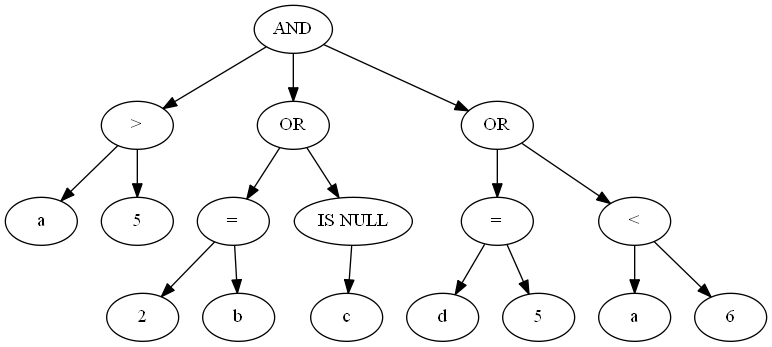
\includegraphics[scale=0.6]{Bilder/sort_1.png}
\caption{Sortierbeispiel: Ausgangsbaum}
\label{fig:sort_1}
\end{figure}

Wir führen zunächst den rekursiven Abstieg bis zu den Blattknoten durch. Wir steigen dann rekursiv auf und betrachten dabei jeweils Knoten, die Kindknoten besitzen. Als erstes Treffen wir dabei auf den Teilbaum, der den Ausdruck \verb|a > 5| repräsentiert. Da der Operator \verb|>| nicht kommutativ ist, können wir die Reihenfolge der Kinder nicht ändern und fahren weiter fort. Im rekursiven Aufstieg treffen wir jetzt auf den Teilbaum, der den Ausdruck \verb|2=b| repräsentiert. Da \verb|=| kommutativ ist, sortieren wir nun die Kinder Anhand ihrer \verb|order()|-Werte. Dabei stellt sich heraus, dass \verb|order(b) = 1 < 2 = order(2)| und damit müssen die Kinder getauscht werden. Wir erhalten den Ausdruck: \verb|b=2|. 
Wir erreichen nun den Teilbaum, der den Ausdruck \verb|(b=2) OR (c IS NULL)| repräsentiert. Da aber \verb|order(=) < order(IS NULL)| ist, müssen wir die Kindknoten nicht vertauschen.
Wir fahren mit dem rekursiven Aufstieg fort und stoßen auf den Teilbaum, der \verb|d=5| repräsentiert. Da \verb|order(d) > order(5)| müssen wir die Kindknoten nicht tauschen. Wir fahren fort und treffen auf den Ausdruck \verb|a < 6| der ebenfalls nicht abgeändert werden kann, da \verb|<| nicht kommutativ ist. 
Beim Aufstieg stoßen wir nun auf den Ausdruck \verb|(d=5) OR (a<6)|. Hier müssen wir eine Vertauschung der Kindknoten durchführen, da \verb|order(=) > order(<)|. Wie in Abbildung \ref{fig:sort_step1} zu erkennen, erhalten wir den Ausdruck \verb|(a<6) OR (d=5)|.

\begin{figure}[H]
\centering
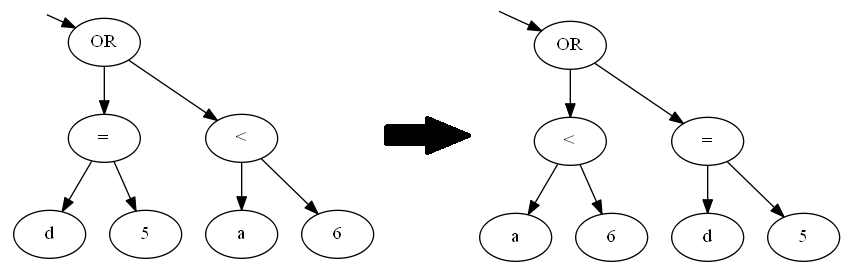
\includegraphics[scale=0.5]{Bilder/sort_step1.png}
\caption{Sortierbeispiel: Umsortierung der Teilbäume}
\label{fig:sort_step1}
\end{figure}

Nun treffen wir auf die zweite Ebene des Baumes und die Teilbäume mit den Wurzeln \verb|>, OR| und \verb|OR|. Da \verb|order(OR) < order(>)| gilt, ist klar, dass der Teilbaum mit \verb|>| als Wurzelknoten nach ganz rechts rücken muss. Noch zu klären ist welcher der beiden Teilbäume mit \verb|OR| als Wurzel als erstes Kind von \verb|AND| erscheint. Dazu müssen wir die schrittweise Tiefensuche auf beiden Bäumen ausführen. Wie wir in Abbildung \ref{fig:sort_step2} dabei feststellen können, unterscheiden sich die Knoten bereits in der ersten Iteration der Tiefensuche.

\begin{figure}[H]
\centering
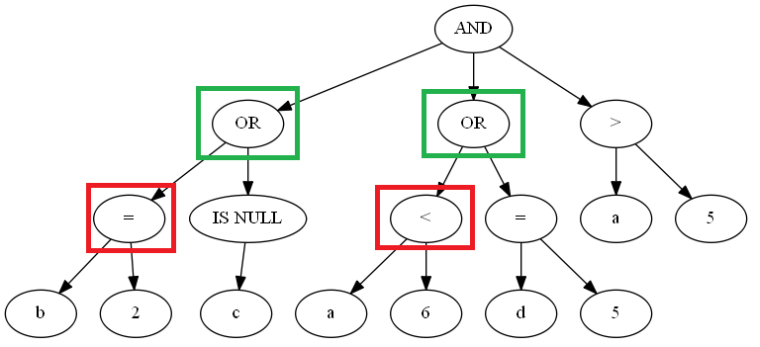
\includegraphics[scale=0.55]{Bilder/sort_step2.png}
\caption{Sortierbeispiel: Schrittweise Tiefensuche}
\label{fig:sort_step2}
\end{figure}

 Da \verb|order(<) < order(=)| müssen wir die Teilbäume mit \verb|OR| als Wurzel ebenso tauschen. Wir erhalten dann den Baum, der in Abbildung \ref{fig:sort_zwischen4} zu sehen ist.

\begin{figure}[H]
\centering
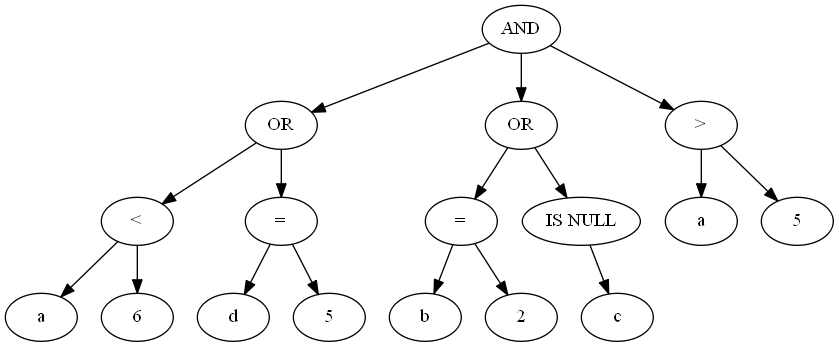
\includegraphics[scale=0.55]{Bilder/sort_zwischen4.png}
\caption{Sortierbeispiel: Ende des Sortierens}
\label{fig:sort_zwischen4}
\end{figure}

Ist das Sortieren abgeschlossen, entfernen wir noch unnötige Duplikate. Haben die Operatoren \verb|AND| oder \verb|OR| zwei gleiche Operanden $o_1,o_2$, die äquivalent sind ($T(o_1) \equiv T(o_2)$), so können wir einen der beiden Operanden streichen. Gleiches gilt für den Operator \verb|OR|. Durch die Sortierung stehen solche Duplikatskandidaten immer nebeneinander. Wir durchsuchen den Baum daher iterativ nach Duplikaten und entfernen diese.

\subsection{GROUP BY / HAVING}

Bisher haben wir den SELECT-, FROM- und WHERE-Teil einer SQL-Anfrage bearbeitet. Anfragen, die einen GROUP BY-Teil enthalten müssen auch nach festen Regeln angepasst werden. Da die Reihenfolge innerhalb dieses Teils unwichtig ist, sortieren wir die Spaltennamen lexikographisch. Die Tupelvariablen sind bereits automatisch benannt nach dem Schema \verb|aN| mit $N\in \{1,2,...\}$ (siehe Unterabschnitt \ref{subsec:from}).

Der HAVING-Teil wiederum ähnelt von seiner Struktur dem WHERE-Teil. Es handelt sich ebenso um einen komplexeren Ausdruck. Wir behandeln daher den HAVING-Teil so, wie den WHERE-Teil im Unterabschnitt \ref{subsec:where}.

Nicht wichtig für die einheitliche Anpassung ist, ob die Tabellen bzw. Aggregationsfunktionen im GROUP BY-Teil auch im SELECT-Teil vorkommen. Dies könnte aber auf einen ungewollten Fehler des Lernenden hinweisen. Diese Information wird daher im Preprocessing (siehe Abschnitt \ref{subsec:preprocessing}) mit aufgenommen. 

\subsection{ORDER BY}

Der ORDER BY-Teil kann nicht im Sinne der Standardisierung angepasst werden. Die hier angegebene Reihenfolge kann nicht verändert werden ohne den Sinn des Ausdruckes zu ändern. Die Anpassung beschränkt sich also auf das Umbenennen der Tupelvariablen, wie es im Unterabschnitt \ref{subsec:from} beschrieben ist.

Interessant für das Preprocessing sind allerdings andere Informationen über ORDER-BY. So merken wir uns, ob die Anfrage ORDER BY-Klauseln mit einem expliziten ASC enthält, da dies unnötig ist.

Weiterhin ist es möglich die Nummer der Spalte, anstatt den Spaltennamen bei der Sortierung anzugeben. Wir ersetzten dabei die Nummer mit dem korrespondierendem Spaltennamen. Wenn in der Aufgabe notiert wurde, dass die Reihenfolge der Spalten egal ist, dann wurden die Einträge unter \verb|SELECT| bereits in Abschnitt \ref{subsec:select} sortiert. Wir müssen also diese Ersetzung vor dieser Sortierung durchführen, da sich sonst die Spaltennummern ändern. Im Programm realisieren wir dies dadurch, dass wir stets die unangetastete Originalanfrage mit abspeichern.

\subsection{Aggregatsfunktionen}

Die Aggregationsfunktionen \verb|MIN()| und \verb|MAX()| benötigen niemals ein \verb|DISTINCT|. Dennoch ist es nicht falsch. Eine Anfrage, die also \verb|DISTINCT| unter diesen Aggregationsfunktionen benutzt, kann dennoch semantisch äquivalent mit der Musterlösung sein. Im Zuge des Standardisierungsprozesses entfernen wir \verb|DISTINCT| innerhalb von \verb|MAX()| und \verb|MIN()|.

Gibt es innerhalb von \verb|COUNT()| kein \verb|DISTINCT| und kann das Argument von \verb|COUNT()| nicht null sein, so ist die Schreibweise \verb|COUNT(attribute)| äquivalent zu \verb|COUNT(*)|. Wir untersuchen daher alle \verb|COUNT()|-Funktionen auf diese Eigenschaften und ersetzen das Argument ggf. zu \verb|*|.

\subsection{Selbstverbunde}

Bevor wir alle Schritte zusammenfassen, möchten wir uns mit Selbstverbunden beschäftigen. Dazu betrachten wir das folgende Beispiel. Dies ist konstruiert und dient nur zur Veranschaulichung eines Problems.

\begin{verbatim}
Musterlösung:
SELECT * FROM emp e, emp f, dept d WHERE e.sal < 1000 AND e.id = f.id

Anfrage des Lernenden:
SELECT * FROM emp e, emp f, dept d WHERE f.sal < 1000 AND e.id = f.id
\end{verbatim}

Wir bemerken, dass beide Anfragen semantisch äquivalent sind. Allerdings prüfen wir in der Musterlösung das Gehalt mit der ersten Tupelvariable und in der Anfrage des Lernenden mit der zweiten Tupelvariable. Unser Programm erkennt daher keine Äquivalenz zwischen beiden Anfragen. Problem ist hierbei der Selbstverbund. Wir können daher im \verb|WHERE|-Teil die Tupelvariablen $e$ und $f$ beliebig tauschen und erhalten immer das gleiche Ergebnis. 

Wir können Selbstverbunde erhalten, indem wir aus einer Anfrage mit Selbstverbund, mehrere Anfragen konstruieren. Dabei permutieren wir für jede erstellte Anfrage die Tabellen unter \verb|FROM| und substituieren dann im \verb|WHERE, GROUP BY| und \verb|ORDER BY|-Teil die Tupelvariablen gemäß der jeweiligen Permutation. Um den Prozess zu verdeutlichen, betrachten noch einmal unser Beispiel. 

Wir erstellen aus dem \verb|FROM|-Teil eine Liste der Tupelvariablen: \verb|[e, f, d]|. Dann gruppieren wir die Liste, so dass sich alle gleichen Tabellen in einer Gruppe befinden: \verb|[ [e, f], [d] ]|. Nun erstellen wir alle Permutationen, indem alle inneren Gruppen permutiert werden. Danach entfernen wir die Gruppierungen wieder und erhalten die folgenden, permutierten Listen:
\begin{verbatim}
[ [e, f], [d] ]  =>  [ e, f, d ]
[ [f, e], [d] ]  =>  [ f, e, d ]
\end{verbatim}

Auf Grundlage dieser Listen, erzeugen wir Substitutionen. Wir substituieren jeweils ein Element aus der Originalliste durch ein Element der erzeugten Permutationslisten. In unserem Fall entstehen dann folgende Substitutionen:

\begin{lstlisting}[mathescape]
$\sigma_1$ = [ e/e, f/f, d/d ]
$\sigma_2$ = [ e/f, f/e, d/d ]
\end{lstlisting}

Diese Substitutionen wenden wir nun auf den \verb|WHERE|-Teil unserer Musterlösung an und erhalten:

\begin{lstlisting}[mathescape]
Musterloesung 1 $(\sigma_1)$:
SELECT * FROM emp e, emp f, dept d 
WHERE e.sal < 1000 AND e.id = f.id 

Musterloesung 2 $(\sigma_2)$: 
SELECT * FROM emp e, emp f, dept d 
WHERE f.sal < 1000 AND f.id = e.id 

Musterloesung 2 ($\sigma_2$, sortiert): 
SELECT * FROM emp e, emp f, dept d 
WHERE f.sal < 1000 AND e.id = f.id 
\end{lstlisting}
\begin{verbatim}
Anfrage des Lernenden (unverändert):
SELECT * FROM emp e, emp f, dept d WHERE f.sal < 1000 AND e.id = f.id
\end{verbatim}


Zu beachten ist, dass in Anfrage 2 auch das Verbundskriterium getauscht wird. Aufgrund unserer Sortierordnung, fällt diese Vertauschung dann aber nicht mehr auf, wie wir in Anfrage 3 sehen können. Weiterhin beobachten wir, dass die unveränderte Anfrage des Lernenden nun auf eine der entstandenen Musterlösungen passt.

\subsection{Abschluss}

Wir fassen die einzelnen Schritte noch einmal kurz zusammen: Zunächst haben wir den \verb|FROM|-Teil der Anfrage vereinheitlicht, indem wir einheitliche Tupelvariablen erzeugt haben, nachdem alle Tabellen im \verb|FROM|-Teil lexikographisch sortiert wurden. Alle neu erzeugten Tupelvariablen wurden im Rest der Anfrage korrekt eingesetzt bzw. ersetzt. Finden wir in diesem Schritt im \verb|FROM|-Teil bereits zwei gleiche Tabellen mit unterschiedlichen Tupelvariablen, so könnte ein Selbstverbund dadurch entstehen. Um mehrdeutigen zu vermeiden, erzeugen wir eine Kopie der vorliegenden Anfrage und vertauschen die gleichen Tabellennamen im \verb|FROM|-Teil. Wir erhalten somit für jeden Selbstverbund einen zusätzlich zu untersuchenden Baum. Am Ende prüfen wir ob einer dieser Bäume syntaktisch äquivalent ist mit einem der erzeugen Bäume, der zweiten Anfrage. Danach haben wir den \verb|WHERE|-Teil bearbeitet. Wir haben zunächst unnötige Klammern entfernt und die Formeln in die KNF überführt. Danach haben wir einfache syntaktische Varianten ersetzt um eine einheitlichere Darstellung zu erhalten. Dazu gehörte es auch Unteranfragen aufzulösen oder, wenn nicht möglich, in eine \verb|EXISTS|-Unteranfrage zu überführen. Eine der letzten Schritte war das Behandeln der Vielfalt der Operatoren. Hier haben wir für alle nicht-kommutativen Operatoren ihre alternativen Schreibweisen konjunktiv-verknüpft mit in die Formel aufgenommen. Nach diesem Schritt müssen wir nun die KNF wiederherstellen, da diese durch hinzufügen von \verb|AND|-Knoten zerstört sein kann. Schlussendlich haben wir den gesamten \verb|WHERE|-Teil sortiert, um eine Vereinheitlichung zu erreichen. Anschließend sortierten wir die Attribute innerhalb des \verb|GROUP BY|-Statements lexikographisch. Der Ausdruck im \verb|HAVING|-Teil, wurde genauso behandelt wie der Ausdruck des \verb|WHERE|-Teils. 

\section{Weitere Betrachtungen}

\subsection{JOINS}
\label{subsec:joins}

Wir betrachten in diesem Abschnitt die Behandlung von JOINs. Wir untersuchen wie wir die unterschiedlichen Verbundstypen vereinfachen oder in eine einheitliche Form umwandeln können. Weiterhin interessiert uns die Frage, wie wir unnötige JOINs erkennen können. Wir diskutieren in wie weit eine automatische Entfernung von unnötigen JOINs Sinn macht und wie das Feedback für den Lernenden aussehen kann.

Vorab möchten wir bemerken, dass die Standardisierung und Eliminierung von JOINs eine fortgeschrittene Strategie darstellt. Diese wird daher nicht im Prototypen auftauchen.

\subsubsection*{CROSS JOIN}

Ein \verb|CROSS JOIN| zweier Relationen liefert das kartesische Produkt beider zurück. Das Schlüsselwort \verb|CROSS JOIN| unter \verb|FROM| markiert diesen. Das Schlüsselwort kann allerdings auch weggelassen und durch ein Komma ersetzt werden. Um eine einheitliche Darstellung dieses Verbundtypes zu gewährleisten, werden wir das Schlüsselwort \verb|CROSS JOIN| ersetzen, so dass wir eine Liste von Tabellen unter \verb|FROM| erhalten, welche mit Komma getrennt sind.

\subsubsection*{NATURAL JOIN}

Ein natürlicher Verbund (NV) ist ein Verbund im \verb|FROM|-Teil. Er wird markiert durch die Schlüsselworte \verb|NATURAL JOIN|. Der Verbund zweier Relationen erfolgt über die Attribute, die in beiden Relationen die gleiche Bezeichnung haben. Gibt es keine solchen Attribute, ist das Ergebnis das kartesische Produkt beider Relationen.

Es gibt zwei Möglichkeiten natürliche Verbunde zu standardisieren. Die erste Möglichkeit besteht darin,   alle Verbundskriterien zu durchsuchen. Stellt man fest, dass die Attribute bei einem Verbundskriterium identisch sind, so handelt es sich um einen natürlichen Verbund. Man könnte diese Kriterien nun streichen und mit dem Schlüsselwort \verb|NATURAL JOIN| explizit kennzeichnen, dass es sich um einen NV handelt. Ein erstes Problem bei dieser Methode ist, dass die Formel unter \verb|WHERE| sehr komplex sein kann. Es ist generell unentscheidbar, ob Verbundskriterien in der Formel auftauchen, da sie auch transitiv-impliziert sein können. Ein zweites Problem ist das folgende Szenario. Angenommen der Lernende L reicht eine Lösung ein, die einen natürliche Verbund zwischen \verb|t1| und \verb|t2| explizit enthält. Weiterhin gibt es kein namensgleiches Attribut in \verb|t1| und \verb|t2|, so dass der natürliche Verbund im Prinzip ein kartesisches Produkt ist. In der Musterlösung stehen \verb|t1| und \verb|t2| nur unter \verb|FROM| um eben dieses Produkt zu erzeugen. Die Methode 1 würde nun gar keine Anpassung machen, da es kein Kriterium für einen potentiellen natürlichen Verbund in der Anfrage des L findet. Als Folge können wir die beiden Anfragen nicht matchen, obwohl beide das gleiche tun.

Die zweite Möglichkeit besteht darin explizite natürliche Verbunde umzuschreiben, in dem wir das Schlüsselwort \verb|NATURAL JOIN| entfernen und beide Relationen durchsuchen nach gleichnamigen Attributen. Der Vorteil zur ersten Methode ist, dass wir immer entscheiden können, ob zwei endliche Relationen zwei gleichnamige Attribute besitzen. Haben wir dann solche Attribute gefunden, so fügen wir diese explizit als Verbundskriterien ein. Haben wir keine solche Kriterien gefunden, handelt es sich um ein kartesisches Produkt. Wir fügen in diesem Fall die zweite Tabelle unter \verb|FROM| hinzu und eliminieren das Schlüsselwort \verb|NATURAL JOIN|.

Beide Methoden haben einen gewissen Aufwand zu bewältigen, allerdings haben wir schon bemerkt, dass Methode 1 unentscheidbare Probleme mit sich bring. Bei Methode 1 müssen wir alle Verbundskriterien durchsuchen. Die Formel kann komplex sein und außerdem ist durch mögliche transitiv-implizierten Gleichungen nicht entscheidbar, ob Verbundskriterien existieren. In Methode 2 müssen wir zwei Relationen paarweise nach gleichnamigen Attributen durchsuchen, was bei endlichen Relationen immer entscheidbar ist.
Aus diesen Gründen entscheiden wir uns für Methode 1. Weil wir den \verb|NATURAL JOIN| unter \verb|FROM| also auflösen, schreiben wir diesen gleich als \verb|INNER JOIN| unter die \verb|WHERE|-Bedingung, wie das  Beispiel \ref{bsp:natjoin} zeigt (angenommen \textit{table1} und \textit{table2} haben beide eine gleichnamige Spalte namens \textit{id}).

\begin{figure}
\begin{verbatim}
Vorher:
SELECT t1.col1 FROM table1 t1 NATURAL JOIN table2 t2

Danach:
SELECT t1.col1 FROM table1 t1, table2 t2 WHERE t1.id=t2.id
\end{verbatim}
\caption{Beispiel: Standardisierung eines natürlichen Verbundes}
\label{bsp:natjoin}
\end{figure}

\subsubsection*{OUTER JOIN}

Bei einem \verb|OUTER JOIN| unterscheiden wir zwischen einem \verb|LEFT OUTER JOIN| und einem \verb|RIGHT OUTER JOIN|. Ein \verb|FULL OUTER JOIN| ist die Verbindung, also ein \verb|UNION| vom linken und rechten \verb|OUTER JOIN|. Wir betrachten daher exemplarisch zunächst den \verb|LEFT OUTER JOIN|, da sich die Betrachtungen dann äquivalent auf den rechten Verbund und damit auf den \verb|FULL OUTER JOIN| übertragen lassen.

Zunächst ist zu klären, wie der \verb|OUTER JOIN| alternativ formuliert werden kann. Dazu gehen wir kurz darauf ein, was ein \verb|LEFT OUTER JOIN| genau macht. Die ``linke'' Tabelle wird vollständig aufgeführt. Dann wird jeder Eintrag der Tabelle sukzessive betrachtet. Gibt es im aktuellen Eintrag einen Verbundspartner in der ``rechten'' Tabelle (vorgegeben durch das Verbundskriterium), dann werden die Daten der ``rechten'' Tabelle an den Eintrag angehangen. Ist dies nicht der Fall, wird der Eintrag mit \textit{NULL} Einträgen aufgefüllt. 

Um die Umwandlung eines \verb|LEFT OUTER JOIN| zu demonstrieren, betrachten wir folgendes Beispiel:

\begin{figure}[H]
\begin{verbatim}
SELECT e.empno, e.job, d.dname 
FROM dept d 
LEFT JOIN emp e ON e.deptno = d.deptno 
WHERE d.loc <> 'CHICAGO'
ORDER BY e.empno
\end{verbatim}
\caption{OUTER JOIN Beispiel}
\end{figure}

Wir haben also zwei verschiedene Mengen von Einträgen. Zum einen Einträge, die einen Verbundspartner besitzen und Einträge, die keinen solchen Partner haben. Anbieten würde sich an dieser Stelle die Verwendung einer Vereinigung (\verb|UNION|) der beiden, eben genannten Mengen. Dabei ist die Umwandlung in ein solches Statement mit einem \verb|UNION| keinesfalls trivial und unterliegt einigen Einschränkungen. 

Ziel ist es also zwei SQL-Anfragen zu formulieren, die jeweils für die oben genannten Mengen stehen. Anschließend werden diese Mengen mit einem \verb|UNION| verbunden.

Für die SQL-Anfrage, welche die Menge der Verbundspartner angibt, übernehmen wir zunächst den \verb|SELECT|-Teil. Die zwei Tabellen, die am Verbund beteiligt sind werden im \verb|FROM|-Teil nun als \verb|CROSS JOIN| aufgeschrieben, also mit Komma getrennt. Der \verb|WHERE|-Teil wird ebenfalls vom gegebenen \verb|OUTER JOIN|-Statement übernommen und durch die Angabe des Verbundskriteriums ergänzt.
Wir erhalten also die folgende Anfrage bezüglich unseres Beispiels:

\begin{figure}[H]
\begin{verbatim}
SELECT e.empno, e.job, d.dname 
FROM dept d, emp e
WHERE d.deptno = e.deptno
AND d.loc <> 'CHICAGO'
ORDER BY e.empno
\end{verbatim}
\caption{OUTER JOIN Umwandlung, 1. Teil}
\end{figure}

Nun muss noch die Teilmenge aller Tupel hinzugefügt werden, die keinen Verbundspartner haben. Wir übernehmen zunächst wieder den \verb|SELECT|-Teil der Ursprungsanfrage, ersetzen aber alle Spaltennamen der ``rechten'' Tabelle mit \verb|NULL|, weil diese Werte aufgrund fehlender Verbundspartner nicht belegt sind. Diese Ersetzungen müssen ebenso im \verb|WHERE|-Teil stattfinden. Die rechte Tablle wird aus dem \verb|FROM|-Teil gestrichen. Nun passen wir den \verb|WHERE|-Teil an. Hier könnte man auf die Idee kommen mit einem \verb|NOT IN| Semijoin zu prüfen, dass auch nur Tupel ohne Verbundspartner aufgenommen werden. Erlaubt  das Verbundskriterium in der ``linken'' Tabelle \verb|NULL|-Werte, so würden diese Einträge nicht erscheinen. Bei einem \verb|LEFT OUTER JOIN| sind diese Tupel aber mit erfasst. Es bietet sich daher eine \verb|NOT EXISTS|-Unterabfrage an. 

\begin{figure}[H]
\begin{verbatim}
SELECT NULL, NULL, d.dname
FROM dept d 
WHERE NOT EXISTS(
    SELECT 1 FROM emp e WHERE d.deptno = e.deptno )
AND d.loc <> 'CHICAGO'
ORDER BY e.empno
\end{verbatim}
\caption{OUTER JOIN Umwandlung, 2. Teil}
\end{figure}

Nun müssen beide Anfragen mit einem \verb|UNION ALL| verknüpft werden. Dabei müssen wir das \verb|ORDER BY|-Statement ausklammern, da dieses erst auf dem Datensatz, der mit \verb|UNION ALL| erzeugt wurde, ausgeführt wird. Unser Endergebnis bezogen auf unser Beispiel lautet also:

\begin{figure}[H]
\begin{verbatim}
SELECT e.empno, e.job, d.dname FROM dept d, emp e
WHERE d.deptno = e.deptno AND d.loc <> 'CHICAGO'
    UNION ALL
SELECT NULL,NULL,d.dname FROM dept d 
WHERE NOT EXISTS(
  SELECT 1 from emp e where d.deptno = e.deptno)
AND d.loc <> 'CHICAGO'
ORDER BY empno
\end{verbatim}
\caption{OUTER JOIN Umwandlung, finaler Schritt}
\end{figure}

Bei diesem Vorgehen kann es passieren, dass bei bestimmten SQL-Anfragen nach der Umwandlung in einen \verb|OUTER-JOIN| klar wird, dass dieser äquivalent zu einem \verb|INNER JOIN| ist. Dazu betrachten wir das Beispiel in Abbildung \ref{fig:outer_s1}.

\begin{figure}[H]
\begin{verbatim}
SELECT e.empno, e.job, d.dname 
FROM dept d 
LEFT JOIN emp e ON e.deptno = d.deptno 
WHERE e.sal > 2000
ORDER BY e.empno
\end{verbatim}
\caption{OUTER JOIN: Spezialfall}
\label{fig:outer_s1}
\end{figure}

Wie wir sehen, taucht im \verb|WHERE|-Teil ein Attribut der ``rechten'' Tabelle auf, was formal zu der Anfrage führen würde, die wir in Abbildung \ref{fig:outer_s2} sehen.

\begin{figure}[H]
\begin{verbatim}
SELECT e.empno, e.job, d.dname FROM dept d, emp e
WHERE d.deptno = e.deptno AND e.sal > 2000
    UNION ALL
SELECT NULL,NULL,d.dname FROM dept d 
WHERE NOT EXISTS(
  SELECT 1 from emp e where d.deptno = e.deptno)
AND NULL > 2000
\end{verbatim}
\caption{OUTER JOIN: Spezialfall Endergebnis}
\label{fig:outer_s2}
\end{figure}

Wie man hier sieht, kann die Bedingung \verb|NULL > 2000| nie erfüllt werden, abgesehen davon, dass es sich um einen Syntaxfehler handelt. Daher muss die zweite Anfrage komplett gestrichen werden und wir erhalten die Anfrage in Abbildung \ref{fig:outjoinspez2}, was nun ein üblicher \verb|INNER JOIN| ist.

\begin{figure}[H]
\begin{verbatim}
SELECT e.empno, e.job, d.dname FROM dept d, emp e
WHERE d.deptno = e.deptno AND e.sal > 2000
\end{verbatim}
\caption{OUTER JOIN: Spezialfall}
\label{fig:outjoinspez2}
\end{figure}


Eine Besonderheit stellt das \verb|GROUP BY|-Statement dar. Dies wurde nicht im Beispiel benutzt, daher betrachten wir nun im Folgenden, wie damit zu verfahren ist.

Wird in der \verb|OUTER JOIN| Abfrage nach mindestens einem Attribut der ``rechten'' Tabelle gruppiert, so müssen wir die Gruppierung in eine weitere Anfrage schachteln. Dazu bauen wir die Anfrage, wie oben beschrieben, auf und streichen das \verb|GROUP BY|-Statement zunächst. Aggregationsfunktion \textit{agg(x)} werden ersetzt zu \textit{x}. Um die dann entstandene, mit \verb|UNION ALL| verknüpfte SQL-Anfrage A schachteln wir eine weitere Anfrage B. Der \verb|SELECT|-Teil von B entspricht dem, der ursprünglichen \verb|OUTER JOIN|-Anfrage. Der \verb|FROM|-Teil von B entspricht der konstruierten Anfrage A. Einen \verb|WHERE|-Teil von B gibt es nicht, da dieser bereits in der Anfrage A eingearbeitet wurde. Ergänzt wird die Anfrage B mit dem \verb|GROUP BY|- und \verb|ORDER BY|-Statement der Ursprungsanfrage.

Existiert im \verb|GROUP BY|-Teil der Originalanfrage kein Attribut der ``rechten'' Tabelle, ist die eben genannte Schachtelung nicht notwendig. Es reicht hier aus den \verb|GROUP BY|-Teil einfach in die Konstruierten Teilanfragen mit einzubeziehen. Grund dafür ist, dass wir disjunkte Gruppierungen in beiden Anfragen erhalten und diese ohne Probleme mit \verb|UNION ALL| vereinigen können.

Dies waren alle notwendigen Schritte um einen \verb|LEFT OUTER JOIN| äquivalent in eine komplexe Anfrage mit \verb|UNION ALL| und Semijoins zu überführen. Zu Bemerken ist an dieser Stelle, dass ein \verb|RIGHT OUTER JOIN| entsprechend behandelt wird, nur mit umgekehrten Seiten. Einen \verb|FULL OUTER JOIN| erhalten wir durch ein \verb|UNION| vom \verb|LEFT OUTER| und \verb|RIGHT OUTER JOIN|. 

Nach dieser Betrachtung müssen wir jedoch feststellen, dass die Umwandlung eines \verb|OUTER JOIN| recht vielschichtig und aufwendig ist. Es ist zwar möglich diesen äquivalent umzuformen, allerdings wird der Ausdruck dadurch enorm aufgebläht. Weiterhin funktioniert diese Umwandlung nur in eine Richtung problemlos, nämlich vom \verb|JOIN| zum \verb|UNION|-Ausdruck. Umgekehrt ist es sehr aufwendig festzustellen, ob ein \verb|UNION ALL| auch ein \verb|OUTER JOIN| ist, da man zum Beispiel Vergleiche mit \verb|NULL|-Werten (wie im Beispiel: \verb|NULL > 2000|) gewöhnlich nicht ausschreibt oder gar entfernt. Unser Programm soll \verb|OUTER JOIN| daher nicht in einen \verb|UNION ALL| Ausdruck umwandeln. Wir beschränken uns in der Praxis also darauf, einen \verb|OUTER JOIN| unter \verb|FROM| rein syntaktisch zu erkennen und nicht umzuwandeln. 

Es sei an dieser Stelle auf die Arbeit \cite{outer2inner} verwiesen, in der ein Verfahren vorgestellt wird, welches \verb|OUTER JOIN| äquivalent in \verb|INNER JOIN| umwandelt. Das Verfahren ist komplex und mehrstufig, kann aber mit allen \verb|OUTER JOIN| umgehen. Der entstandene \verb|INNER JOIN| ist allerdings aufgebläht und nicht mehr lesbar, da er künstlich konstruiert ist. Im Rahmen unserer Arbeit interessiert dieser Fakt nur am Rande, im Zuge einer Erweiterung der semantischen Funktionen unseres Programmes, ist dieser Ansatz aber sicherlich erwähnenswert und interessant.

\subsubsection*{INNER JOIN}

Unter einem \verb|INNER JOIN| verstehen wir den Verbund zweier Tabellen unter \verb|FROM|, mit den Schlüsselworten \verb|INNER JOIN|. Ein solcher Verbund kann leicht als \verb|CROSS JOIN| mit Auswahl in der \verb|WHERE|-Bedingung formuliert werden. Dazu entfernen wir den \verb|INNER JOIN| aus dem \verb|FROM|-Teil und erzeugen einen \verb|CROSS JOIN|. Die Verbundbedingungen werden unter \verb|WHERE| eingefügt.

Ein explizit aufgeschriebener \verb|INNER JOIN| kann auch ein \verb|NATURAL JOIN| sein. Da wir solche Verbunde aber auch als \verb|CROSS JOIN| aufschreiben wollen (siehe oben), müssen wir diesen Spezialfall nicht gesondert betrachten. Das folgende Beispiel soll die Umwandlung von \verb|INNER JOIN| verdeutlichen:

\begin{figure}[H]
Eingabe:\\
\verb|SELECT * FROM emp e INNER JOIN dept d ON e.deptno.id = d.deptno|\\

Umwandlung:\\
\verb|SELECT * FROM emp e, dept d WHERE e.deptno = d.deptno|\\
\caption{Umwandlung von INNER-JOIN}
\end{figure}


\subsubsection{JOIN-Eliminierung}

Im vorherigem Abschnitt haben wir bereits alle üblichen Verbunde betrachtet und gezeigt, wie wir diese äquivalent umformen können. Wir haben erreicht, dass alle Verbunde unter \verb|FROM| ersetzt wurden zu \verb|CROSS JOIN| mit Auswahlkriterien unter \verb|WHERE|. Wir möchten daher in diesem Abschnitt auf eine Methode verweisen, mit der es möglich ist überflüssige \verb|INNER JOIN| zu erkennen und zu eliminieren.

Die Methode selbst ist detailliert in \cite{joinelem2} beschrieben und würde den Rahmen dieser Arbeit überschreiten. Daher wollen wir hier nur ein Beispiel hernehmen und es mit der Methode bearbeiten, um zu sehen was die Methode leisten kann.

Der Algorithmus aus \cite{joinelem2} findet redundante Verbunde mit Hilfe von referentiellen Integritätsbedingungen (RI). Dann folgt die Entfernung einer Relation bei dem der Verbund aus Tabellen besteht, die durch eine RI-Bedingung verbunden ist (nachfolgend als RI-Joins bezeichnet) und bei der die Tabelle, die den Primärschlüssel enthält nur im Join referenziert wird. Ein RI-Join besteht natürlicherweise aus einem Primärschlüssel- und einem Fremdschlüsselattribut.

Als visuelles Hilfsmittel verwendet das Verfahren sogenannte Joingraphen $G=(V,E)$. Die Knotenmenge $V$ besteht aus Joinattributen. Eine Kante zwischen zwei Knoten $u,v$ existiert genau dann, wenn $u$ und $v$ Teil eines Joinprädikates sind. Handelt es sich bei dem Join um einen RI-Join, also ein Primär-/ Fremdschlüssel Join, dann sind $u,v$ durch eine gerichtete Kante verbunden, wobei der Pfeil dann vom Fremdschlüsselattribut/Kind zum Primärschlüsselattribut/Eltern geht. Das Bearbeiten der folgenden Beispielanfrage soll zeigen, wie das Verfahren vorgeht. Die Datenbankschemata sind dem TCP-H entnommen und in \cite{partsuppdb} zu finden.

\begin{lstlisting}[mathescape]
SELECT ps.partkey, avg(ps.supplycost)
FROM   supplier s, partsupp ps, customer c, orders o
WHERE  s.suppkey = ps.suppkey 
AND    s.suppkey = c.custkey
AND    c.custkey = o_custkey
AND    o.totalprice >= 100
GROUP BY ps.partkey
\end{lstlisting}

Wir erzeugen zunächst den ersten Joingraphen $G_1$, in dem wir jede Joinbedingung als verbundenes Paar in den Graphen einfügen:

\begin{figure}[H]
\centering
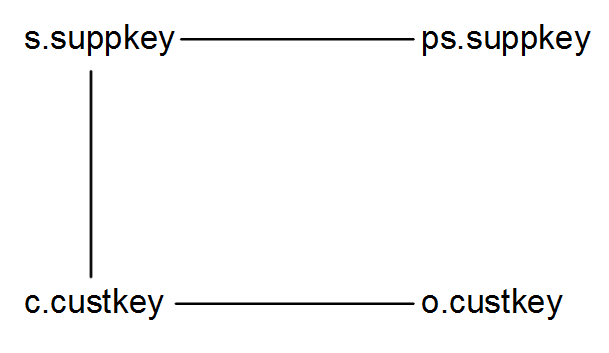
\includegraphics[scale=0.4]{Bilder/joinelem_g1.png}
\caption{$G_1$}
\end{figure}

Wir weisen die RI-Joins aus, in dem wir sie als gerichtete Kanten markieren. Weiterhin fügen wir nun alle transitiv-implizierten Joins als nicht RI-Joins hinzu, also als ungerichtete Kanten und erhalten damit $G_2$:

\begin{figure}[H]
\centering
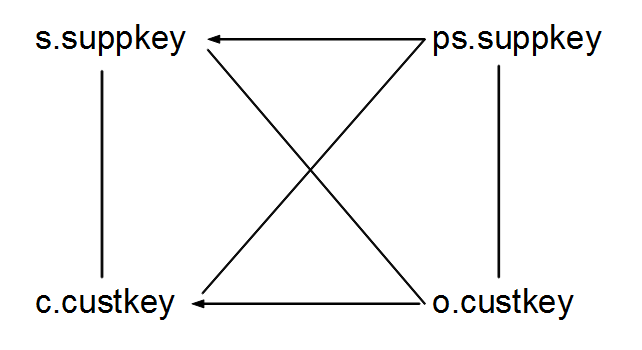
\includegraphics[scale=0.4]{Bilder/joinelem_g2.png}
\caption{$G_2$}
\end{figure}

Im letzten Schritt gehen wir alle Knoten sukzessive durch. Da jeder Knoten ein Attribut repräsentiert, prüfen wir ob das repräsentierte Attribut in einem Nicht-Join Prädikat unter \verb|WHERE|, im \verb|GROUP BY|- oder im \verb|SELECT|-Teil vorkommt. Falls ja, ersetzen wir das Attribut mit einem Attribut eines Verbundspartners, der noch im Graphen existiert. Dann eliminieren wir den Knoten und alle zugehörigen Kanten. In unserem Beispiel kommt weder \verb|s.suppkey| noch \verb|c.custkey| in den genannten Teilen der Anfrage vor und damit können wir diese Entfernen ohne Attributsreferenzen ersetzen zu müssen. Wir löschen diese Attribute aus $G_2$ und erhalten $G_3$ mit nur noch einem, notwendigen Join:

\begin{figure}[H]
\centering
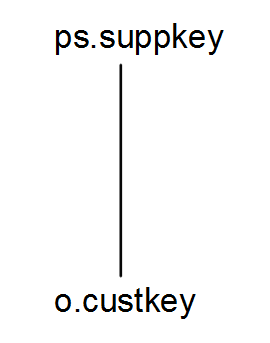
\includegraphics[scale=0.4]{Bilder/joinelem_g3.png}
\caption{$G_3$}
\end{figure}

Wir erhalten also folgende SQL-Anfrage:

\begin{lstlisting}[mathescape]
SELECT ps.partkey, avg(ps.supplycost)
FROM   partsupp ps, orders o
WHERE  o.custkey = ps.suppkey 
AND    o.totalprice >= 100
GROUP BY ps.partkey
\end{lstlisting}


%\section{Komplexität von SQL-Anfragen}

%Durch Standardisierung zweier SQL-Abfragen \verb|query1| und \verb|query2| können wir durch einen syntaktischen Vergleich prüfen, ob es uns möglich war, beide gegeneinander zu matchen. Unabhängig vom Ergebnis dieses Matchings ist für den Lernenden wichtig, wie nah er an der Musterlösung dran war. Folgende Szenarien sind dabei denkbar. 
%
%Im ersten Szenario konnte die SQL-Anfrage des Lernenden nicht mit der SQL-Anfrage der Musterlösung gematcht werden. Der Lernende benötigt nun ein Feedback um seine Fehler zu erkennen und um letztendlich einen neuen Lösungsvorschlag zu machen. 
%
%In einem zweite Szenario konnte die SQL-Anfrage des Lernenden gematcht werden. Während des Standardisierungsprozesses seiner Anfrage, kann es aber sein, dass unnötige Klauseln entfernt wurden. In einem solchen Fall ist es von Interesse dem Lernenden mitzuteilen, dass seine Lösung noch nicht perfekt (im Sinne der Musterlösung) ist. 
%
%Wir wollen im Folgenden nun Kriterien von Metainformationen festlegen. Diese Metainformationen der zwei Anfragen sollen dann jeweils miteinander verglichen werden. Finden wir bei einem solchen Vergleich Unstimmigkeiten in der Anzahl der jeweiligen Informationen, muss dies dem Lernenden mitgeteilt werden.



%\section{Alternativer Ansatz: Elementare Transformationen}

%Der nun vorgestellte Ansatz stellt eine Alternative zur >>Anpassung durch Standardisierung<< dar. Beide %Ansätze haben ähnliche Ideen, sind jedoch in ihrer Umsetzung verschieden. Beim Ansatz der Standardisierung %haben wir zunächst eine SQL-Anfrage genommen und standardisiert. Dies geschah völlig unabhängig zu der zu %vergleichenden, zweiten SQL-Anfrage. Es wurden gewisse allgemeine Regeln aufgestellt und nach diesen wurde jede SQL-Anfrage behandelt und angepasst. Der eigentliche Vergleich geschah dann aufgrund eines Vergleichs der standardisierten Anfragen und dem Vergleich von Metadaten (Anzahl Joins, Anzahl atomarer Formeln, etc.). Ein Nachteil von diesem Ansatz ist, dass wir für jedes mögliche Konstrukt in der SQL-Anfrage auch Regeln im System haben, damit wir jene Konstrukte auch anpassen und standardisieren können. Außerdem findet der Vergleich erst im allerletzten Schritt statt.%
%
%Die >>Anpassung durch elementare Transformationen<< stellt einen intuitiven Ansatz vor. Wir versuchen hier per Backtracking konkret eine Lösung der anderen anzugleichen. Damit haben wir einen konkreten Unterschied zum bisherigen Ansatz. Wir vergleichen die Lösung direkt und umgehen die Vorverarbeitungen. Im Wesentlichen geben wir also ganz allgemeine Regeln an und in jedem Schritt versuchen wir durch Anwendung dieser Regeln die SQL-Anfrage so anzupassen, dass sie auf unsere zu vergleichende Anfrage passt.



\subsection{unnötiges DISTINCT}

Eine interessante Frage ist, ob ein \verb|DISTINCT| wirklich notwendig ist. Dies ist natürlich wichtig für den Vergleich zweier SQL-Anfragen. In \cite{brass2} wurde im Rahmen des SQLLint-Projektes bereits in dem Prototypen ein Checker eingebaut, der prüft ob \verb|DISTINCT| wirklich notwendig ist. Aber auch im Rahmen dieser Arbeit ist es notwendig zu wissen, ob das \verb|DISTINCT| notwendig ist. 

Auf den ersten Blick reicht es aus zu prüfen, ob die Musterlösung ein \verb|DISTINCT| enthält. Allerdings kann es Fälle geben, in denen man anstatt eines \verb|DISTINCT| eine \verb|EXISTS|-Unterabfrage benutzt und daher benötigen wir einen Ansatz, der unabhängig von der Musterlösung entscheidet ob ein \verb|DISTINCT| notwendig ist.  Im Folgenden stellen wir daher einen Algorithmus vor, der erkennt ob die Lösung Duplikate enthalten kann oder nicht. Das allgemeine Frage, ob ein \verb|DISTINCT| notwendig ist, ist unentscheidbar. Deswegen prüft der nachfolgende Algorithmus die hinreichende Bedingung für ein unnötiges \verb|DISTINCT|. Das bedeutet, dass wenn der Algorithmus sagt >>ja, \verb|DISTINCT| ist unnötig<<, können wir sicher sein, dass es tatsächlich unnötig ist. Sagt der Algorithmus allerdings >>nein<< bedeutet dies, nicht notwendigerweise, dass das \verb|DISTINCT| wirklich unnötig ist. 

Der Algorithmus ist nicht in unserem Programm implementiert. Wir beschreibe ihn aber im Folgenden so, dass er in einer Überarbeitung ohne Probleme integriert werden könnte. Der Algorithmus müsste dann in jedem Fall nach der Umwandlung des \verb|WHERE|-Teils in die KNF erfolgen, da dies eine Voraussetzung für den Algorithmus ist.

\subsection{verbale Beschreibung}

Es sei $\mathcal{K}$ die Menge aller Attribute, die als Ausgabespalten unter \verb|SELECT| vorkommen.
Wir fügen im nächsten Schritt nun alle Attribute $A$ zu $\mathcal{K}$ hinzu, für die $A=c$ bzw. $c=A$ in der \verb|WHERE|-Bedingung auftaucht. Hierbei wird, wie bereits erwähnt, vorausgesetzt, dass die Bedingung eine Konjunktion ist. Weiterhin ist zu bemerken, dass Unterabfragen vom Algorithmus ignoriert werden.

Solange eine der folgenden Aktionen zu einer Veränderung unseres Zustands führt, machen wir Folgendes:
\begin{itemize}
\item Wir fügen zur Menge $\mathcal{K}$ Attribute $A$ hinzu, wenn $A=B$ Teil der \verb|WHERE|-Bedingung ist und $B\in \mathcal{K}$ gilt.
\item Enthält $\mathcal{K}$ einen Schlüssel einer Tupelvariable, so fügen wir alle Attribute dieser Variable hinzu.
\end{itemize}

Enthält $\mathcal{K}$ nun von jeder Tupelvariable unter \verb|FROM| einen Schlüssel, so ist das \verb|DISTINCT| sicher überflüssig. Haben wir ein \verb|GROUP BY|-Statement so prüfen wir anstelle dessen, ob alle \verb|GROUP BY|-Spalten in $\mathcal{K}$ enthalten sind. Der folgende Algorithmus ist \cite{sql1folien} entnommen.

\subsection{Algorithmus}

Es sei unsere SQL-Anfrage der Form:

\begin{lstlisting}[mathescape]
SELECT $t_1$, ..., $t_k$
FROM $R_1\ X_1$, ..., $R_n\ X_n$
WHERE $\varphi$
\end{lstlisting}

Es sei $X=\{X_1, ..., X_n\}$ die Menge aller Tupelvariablen. Es sei $G=\{G_1, ..., G_m\}$ die Menge aller \verb|GROUP BY| Spalten.

Die einzelnen Attribute $t_i$ haben die Form $t = X.k$. Dabei ist $X$ eine Tupelvariable und $k$ ein Attribut. Wir bezeichnen die Menge aller $t_i$ mit $\mathcal{K}=\{t_1,...,t_k\}$.

\begin{lstlisting}[mathescape]
$\mathcal{K}$ = $\mathcal{K}\ \cup$ {A}, wenn $A=c$ als Konjunktion in WHERE auftaucht
do 
  $\mathcal{K'}$ = $\mathcal{K}$
  $\mathcal{K'}$ = $\mathcal{K'}\ \cup$ A, wenn $A=B\in$ WHERE-Bedingung und $B\in\mathcal{K}$
  $\mathcal{K'}$ = $\mathcal{K'}\ \cup$ S mit $S=\{b\in X\}$, wenn $t\in \mathcal{K'}$ ein Schluessel ist und t=X.k
while ($\mathcal{K}\ \neq\ \mathcal{K'}$)

if not Anfrage hat GROUP BY Statement:
  foreach $x\in X$ do
    if not ($\exists k\in \mathcal{K'}$ mit $k$ ist Schluessel von $x$)
      break and return NO
    endif
  done

if Anfrage hat GROUP BY Statement:
  foreach $g\in G$ do
    if $g\notin \mathcal{K'}$
      break and return NO
    endif
  done

return YES
\end{lstlisting}


\section{SQL-Anfragen auf externen Datenbanken}

Bis jetzt haben wir verschiedene Methoden und Ansätze diskutiert, die sich auf das Erfüllen der hinreichenden Bedingung, einer semantischen Äquivalenz, konzentriert haben. In den vorherigen Abschnitten dieses Kapitels haben wir festgestellt, dass eine, durch Überführung, erhaltene syntaktische Äquivalenz zweier SQL-Anfragen automatisch deren semantische Äquivalenz bedeutet. Wie Eingangs erwähnt, ist das Problem, zwei SQL-Anfragen auf semantische Äquivalenz zu prüfen, im Allgemeinen nicht entscheidbar. Aus diesem Grund kann es passieren, dass unsere, bisher erarbeiteten Methoden, bei einigen, semantisch äquivalenten, Anfragen keinen Erfolg bringen. Die Anfragen sind dann semantisch äquivalent, aber wir können sie nicht durch unsere Methoden aneinander anpassen. 

Für diese Art von Anfragen prüfen wir eine notwendige Bedingung der semantischen Äquivalenz zweier Anfragen. Für diesen Schritt benötigen wir echte Daten für das, jeweils gegebene, Datenbankschema. Wir führen sowohl die Musterlösung, als auch die Lösung des Lernenden auf einer Datenbank mit realen Daten aus. Wir vergleichen dann die zurückgelieferten Tupel. Unterscheiden sich diese, dann wissen wir, dass die beiden Anfragen nicht semantisch äquivalent sein können. Dabei würde der Unterschied in beiden Antwortmengen das Gegenbeispiel zur Äquivalenz darstellen.

Sind die Antwortmengen identisch für alle vorhandenen Datenbankzustände, ist dies kein sicheres Zeichen dafür, dass die Anfragen semantisch äquivalent sind, da dies nur das notwendige Kriterium, nicht aber ein hinreichendes Kriterium ist. Haben wir also zwei SQL-Anfragen deren semantische Äquivalenz weder durch Standardisierung nachgewiesen, noch durch Tests auf realen Daten widerlegt werden konnte, so wissen wir nicht, ob diese Anfragen sicher äquivalent sind oder nicht. Wir geben den Lernenden dann das Feedback, dass seine Lösung eventuell richtig oder falsch ist. Auch muss der Dozent, oder andere Berechtigte, über solche Lösungen informiert werden. Die berechtigte Person kann dann entscheiden ob die Lösung eine weitere Musterlösung darstellt, oder nicht korrekt ist.

Im Detail gibt es allerdings einige Feinheiten zu beachten, wenn man die Anfragen auf konkreten Datenbanken mit echten Daten ausführen will. Im Folgenden werden wir diese Feinheiten erläutern und mögliche Probleme disktuieren.

\subsection{unterschiedliche DBMS}

Obwohl es, in gewissen Abständen, zur Herausgabe eines Standards für SQL durch die ISO kommt, unterscheiden sich die existierenden DBMS bei der Handhabung und Implementation von SQL-Features. Die aktuellste Version des SQL-Standards ist zur Zeit: SQL:2008. Die verschiedenen Hersteller variieren diesen Standard allerdings, durch Entfernung oder Hinzufügen von Funktionalitäten. Diese Änderungen sind sowohl in der Data Definiton Langauge (DDL), der Data Manipulation Language (DML) als auch der Data Control Language (DCL) zu finden. Wir gehen im Folgenden auf einige Unterschiede ein. Da wir im Hinblick auf diese Arbeit gerne unabhängig von den Herstellern verschiedner DBMS sein wollen, ist für uns Interessant, welche Schnittmenge von Funktionalitäten alle DBMS gemeinsam haben. Nach heutigem Stand können wir sagen, dass DB2, MSSQL, MySQL, Oracle und Informix mindestens den SQL-92 Standard erfüllen. PostgreSQL hat zusätzlich noch das Konzept der Sichten, erlaubt aber nicht diese zu aktualisieren (update). Um diese Restriktion zu umgehen, führt PostgreSQL ein, nicht vom Standard vorgesehenes, Konzept von Regeln ein, auf das wir nicht näher eingehen wollen. Ist unsere Anfrage also SQL-92 konform, so können wir diese ohne Probleme auf allen gängigen DBMS ausführen.

Betrachten wir nun ein paar Unterschiede im Detail. Von den, oben genannten, DBMS verstehen nur PostgreSQL, MySQL und Oracle das Schlüsselwort \verb|NATURAL JOIN| unter \verb|FROM|. \verb|FULL JOIN|, also die Vereinigung eines \verb|LEFT OUTER| und \verb|RIGHT OUTER| Join verstehen alle DBMS, bis auf MySQL. Alle DBMS verstehen aber das explizite kartesische  Produkt, \verb|CROSS JOIN|. Dieser Sachverhalt kommt uns entgegen, da wir versuchen im ersten Teil, der Standardisierung, alle Joins als kartesisches Produkt mit Auswahl zu formulieren, falls das möglich ist. Können wir bestimmte Joins nicht umschreiben, kann es zu Laufzeitfehlern kommen, welche später in diesem Kapitel behandelt werden.

Unterschiede in der DDL behandeln wir nicht, da wir uns im, Rahmen dieser Arbeit, nur mit dem \verb|SELECT|-Statement beschäftigen. Ein wesentlicher Unterschied hierbei besteht in der Sortierung von Werten. Der Standard trifft keine Aussage darüber, wie \verb|NULL|-Werte im Verlgeich zu nicht-\verb|NULL|-Werten sortiert werden sollen. Der Standard beschreibt lediglich die Schlüsselwörter \verb|NULLS FIRST| sowie \verb|NULLS LAST|, um das Verhalten dementsprechend zu erzwingen. In der Implementation haben die Hersteller sich allerdings entscheiden müssen, was im default-Fall zu tun ist. In den Systemen PostgreSQL, DB2 und Oracle werden \verb|NULL|-Werte mit höherer Priorität als nicht-\verb|NULL|-Werte behandelt. Dementsprechend behandeln MSSQL, Informix und MySQL die \verb|NULL|-Werte niedriger, als die nicht-\verb|NULL|-Werte. Bei Oracle tritt zusätzlich die Besonderheit auf, dass ein leerer String die gleiche Priorität hat, wie ein \verb|NULL|-Wert. 

Weitere Unterschiede zwischen den DBMS treten auf in Bezug auf das Schlüsselwort \verb|LIMIT n|, welches bewirkt, dass nur die ersten $n$ Datensätze ausgegeben werden. Lediglich MySQL und PostgreSQL kennen dieses Schlüsselwort. Bei allen anderen DBMS muss diese Anforderung durch Verwendung der \textit{row-number} umgesetzt werden. 

Weitere Unterschiede haben die DBMS bei Verwendung vom \verb|BOOLEAN|-Datentyp, dem \verb|UNIQUE|-Constraint, der Konkatenation von Strings, dem Schlüsselwort \verb|LOCALTIMESTAMP|, der Funktion \verb|SUBSTRING| und dem Datentyp \verb|TIMESTAMP|. Es würde zu weit führen alle Unterschiede genau zu betrachten. Nachzulesen sind die genauen Unterschiede unter \cite{sqldiff1}

Wichtig für unsere Arbeit ist, dass wir keine Probleme zu erwarten haben, wenn eine Anfrage SQL-92 konform ist. Sollte dies nicht der Fall sein werden wir, mit großer Wahrscheinlichkeit, einen Laufzeitfehler oder einen Fehler beim Parsen der Anfrage erhalten.

\subsection{Visualisierung von Ergebnistupeln}

Wir wollen zwei SQL-Anfragen auf einer konkreten Datenbank ausführen. Nun müssen wir die entstandenen Ergebnismengen miteinander vergleichen. Dabei wollen wir in diesem Abschnitt diskutieren wie dies am sinnvollsten Geschehen soll. 

Der erste Ansatz ist es, beide Ergebnismengen iterativ zu vergleichen. Wir gehen also beide Mengen Schritt für Schritt durch. Treffen wir dabei auf unterschiedliche Elemente, so geben wir an in welchem Tupel sich beide Mengen unterscheiden und beenden den Vergleich. Wir müssen sicher gehen, dass die Reihenfolge der Spalten und Zielen dabei keine Probleme verursacht.

Interessant sind dabei sowohl die Reihenfolge der Spalten, als auch die Sortierung der Tupel eine Rolle. Wir haben die Sortierung der Spalten bereits im Abschnitt \verb|SELECT|-Teil behandelt. Spielt die Reihenfolge keine Rolle, so sind die Items im \verb|SELECT|-Teil bereits lexikographisch sortiert. Andernfalls ist die Reihenfolge fix und wir müssen sie so nehmen, wie wir sie erhalten.

Für eine eindeutige Reihenfolge der Tupel haben wir allerdings bisher nicht gesorgt. Wir müssen hier mehrere Fälle betrachten. 

Enthält die Musterlösung und die Lösung des Lernenden kein \verb|ORDER BY|, müssen wir uns um die Reihenfolge nicht weiter kümmern, da jedes DBMS deterministisch eine Reihenfolge auswählen wird. Diese Reihenfolge ist dann insbesondere für beide Anfragen identisch, da deterministisch.

Der zweite Fall zeichnet sich dadurch aus, dass die Musterlösung kein \verb|ORDER BY| enthält, die Lösung des Lernenden enthält aber ein solches. Wir können dann davon ausgehen, dass die Reihenfolge nicht von Bedeutung ist, denn sonst würde die Musterlösung ein \verb|ORDER BY| enthalten. Wir könnten nun entweder das \verb|ORDER BY| aus der Lösung des Lernenden entfernen, oder das \verb|ORDER BY| des Lernenden in die Musterlösung einfügen. Im letzten Fall kann es Probleme geben, wenn die Lösung des Lernenden Spalten im \verb|ORDER BY| enthält, die in der Musterlösung nicht vorkommen. Wir entscheiden uns daher zur Entfernung des \verb|ORDER BY| aus der Lösung des Lernenden, bevor wir die Anfragen auf der realen Datenbank ausführen. Der Lernende erhält natürlich dennoch einen Hinweis, dass er ein \verb|ORDER BY| verwendet, die Musterlösung aber nicht. Solche Informationen werden ja bereits im Preprocessing gesammelt und gehen dadurch nicht verloren.

Der dritte Fall wäre dann genau umgekehrt. Hier hat also die Musterlösung ein \verb|ORDER BY|-Statement, die Lösung des Lernenden aber nicht. Hier ist offensichtlich eine Reihenfolge gewünscht. Wir werden daher keine Anpassung in einem solchen Fall durchführen. Unterscheiden sich die Musterlösung und die Lösung des Lernenden nur durch das \verb|ORDER BY|-Statement, erhält der Lernende ohnehin eine Meldung, dass der Rest der Anfrage übereinstimmt, so wie im Bereich Preprocessing erläutert.

Der letzte Fall ist für uns nicht relevant. In beiden Anfragen befindet sich dann ein \verb|ORDER BY| und daher können wir auch keine Anpassungen vornehmen. 

Nachdem wir dann die zwei Anfragen auf der Datenbank ausgeführt haben erhalten wir zwei Ergebnistupel. Stellt sich durch einen schrittweise Vergleich heraus, dass beide Ergebnismengen identisch sind, müssen wir dem Studenten mitteilen, dass es nicht entscheidbar ist, ob seine Lösung korrekt ist oder nicht. In einem solchen Fall muss der Dozent entweder eine Mail erhalten, um die Lösung manuell zu prüfen, oder dem Studenten wird angezeigt, dass er diese Lösung doch in der nächsten Übung vorstellen soll, um deren Korrektheit zu prüfen.

Sind die Ergebnismengen aber nicht gleich, so zeigen wir beide Tupel in Tabellenform nebeneinander an. Der Lernenden kann dann schnell und übersichtlich erkennen, welche Tupel er mit seiner Anfrage zurückliefert und welche Tupel ihm fehlen bzw. zu viel sind.

\subsection{Behandeln von Fehlern}

Bei der Ausführung von SQL-Anfragen auf realen Datenbanken können verschieden Fehler auftreten. Wir möchten nun kurz untersuchen welche Arten von Fehlern wir erwarten können und wie wir diese behandeln wollen. Der Begriff >>Fehler<< ist in diesem Sinne auch etwas weiträumiger zu verstehen, wie wir gleich merken werden.

Einer der typischsten Fehler ist der Syntaxfehler. Der Lernende hat also eine Lösung angegeben, die nicht in das Syntaxschema einer SQL-Anfrage passt. Die Hauptursachen für solche Fehler sind falsche Anordnung von Schlüsselwörtern oder gar >>Rechtschreibfehler<<. Jedoch kann es auch sein, dass der Lernende Syntax benutzt hat, welche nur ein bestimmtes SQL-System versteht, \mbox{z. B.} PostgreSQL. Wird die Anfrage aber auf einer Oracle Datenbank ausgeführt, versteht das DBMS diese Anfrage eventuell nicht und es kommt zu einem Syntaxfehler, der auf einem anderen DBMS keiner wäre. Wir könnten den Fehler verhindern, in dem wir in einem vorherigen Schritt prüfen, ob die Anfrage SQL-92 konform ist. Eine andere Lösung ist es, zu jeder Anfrage zu speichern, für welches konkretes DBMS sie gedacht ist. Dann könnte man sich sicher sein, dass der Syntaxfehler auch einen Fehler für alle SQL-Systeme darstellt. Wenn man keine gesonderte Behandlung in Betracht zieht, so kann man den Fehler, wie üblich, dem Nutzer anzeigen mit dem Vermerk, dass der Syntaxfehler eventuell zu DBMS spezifisch ist. In unserem Prototypen reichen wir derartige Syntaxfehler an den Nutzer weiter.

Ein weiterer Fehlertyp ist der semantische Fehler. Wie bereits, in der Einführung dieser Arbeit, erwähnt, ist dies ein Fehlertyp, der schwer zu entdecken ist. Typische Vertreter sind inkonsistente Bedingungen, also \verb|WHERE|-Bedingungen, die entweder immer die leere Menge liefern, oder die immer die gesamten Tabellen als Ergebnistupel liefern, da die \verb|WHERE|-Bedingung allgemeingültig ist (Tautologie). Die eben genannten Fälle erkennt unser Programm, da es mit der Methode \verb|eval| die Ausdrücke so weit möglich auswertet. Andere semantische Fehler, wie unnötige JOINs und unnötiges DISTINCT wurden bereits im Kapitel \ref{chap:theorie} behandelt. Unser Programm wird davon allerdings nichts umsetzen, da es einen größeren Aufwand darstellt diese Methoden zu implementieren. Es gibt weitere semantische Fehler, die unser Programm nicht berücksichtigt. Hier sei verwiesen auf die Arbeit \cite{brass2}. 

In Hinblick auf syntaktische und semantische Fehler sollten wir uns fragen, welche Anfrage wir, zur Ausführung auf der realen Datenbank, einsetzen wollen. Zur Wahl stehen dabei die Anfrage, die der Lernende eingibt und die Anfrage, die unser Programm im ersten Schritt durch Standardisierung erzeugt. 

Da wir, bei der Ausführung der Anfragen auf realen Datenbanken, darauf bedacht sind, so wenig Fehler wie möglich zu erzeugen, ist es am sinnvollsten, die standardisierte Anfrage zu verwenden. Der Lernende bekommt in jedem Fall Hinweise, wenn bei der Standardisierung semantische oder syntaktische Besonderheiten gefunden wurden. hat der Student \mbox{z. B.} eine Tautologie als \verb|WHERE|-Bedingung aufgeschrieben, so kann das unser Programm erkennen. Der Lernende erhält den Hinweis, dass seine Bedingung überflüssig ist und auf der realen Datenbank lassen wir dann, die schon verkürzte Fassung laufen. 

Ein letzter Fehlertyp bilden die Laufzeitfehler. Da wir solche Fehler nur schwer oder gar nicht im Vorfeld erkennen können, sind wir gezwungen die Fehlermeldung an den Lernenden weiterzugeben. Diese Fehlermeldung werden vom konkreten DBMS erzeugt und können mitunter unverständlich sein. Jedes DBMS hat dabei auch eine eigene Formulierung für die gleichen Laufzeitfehler. Es bietet sich daher an, eine Art Wörterbuch für Fehlermeldungen zu verwenden. Tritt ein bestimmter Fehler in einem DBMS auf, so wird dieser >>übersetzt<< in eine, von uns standardisierte, Fehlermeldung. So können wir sicher sein, dass der Student beim gleichen Fehler, die gleiche Meldung erhält, unabhängig vom DBMS.

%Parser, Java Version, Eigener Parser, Anbindung an fremde DB Oracle, Mysql, etc.

\chapter{Praktische Umsetzung}
\label{chap:praxis}
\section{Anforderungen}

Das zu entwickelnde Programm wird online per Java Servlets zur Verfügung gestellt. Als Webserver wird der Tomcat eingesetzt. Folgende Funktionalitäten sollen umgesetzt weden:

\begin{itemize}
\item Loginsystem für Lernenden und Betreuer
\item Grafische Oberfläche
\item Eintragen von neuen Übungsaufgaben bestehend aus:
	\begin{itemize}
	\item Sachtext /Aufgabenstellung
	\item Musterlösung(en)
	\item Angabe von realen Datenbanken mit Testdaten
	\item Einteilung in Kategorie
	\end{itemize}
\item Löschen und Bearbeiten von Übungsaufgaben
\item Erstellen, Bearbeiten und Löschen von Kategorien
\item Lösen von Übungsaufgaben durch Angabe einer SQL-Anfrage
\item Tracking von Lösungsversuchen (Versuch, AufgabenID, Timestamp, UserID)
\item Tracking von Usern und letzten Aktivitäten
\item Tracking von Fehlern/ Fehlversuchen pro Aufgabe/User
\end{itemize}

\chapter{Schlussteil}
\label{chap:ausblick}

\section{Zusammenfassung}

Die Aufgabenstellung für diese Arbeit war es, Methoden zu entwickeln mit denen man in der Lage ist, zwei SQL-Anfragen miteinander zu vergleichen. Dabei sollte herausgefunden werden, ob die beiden Anfragen semantisch äquivalent sind und damit immer die gleichen Ergebnistupel produzieren. Entwickelte Methoden sollten dann in einem Programm realisiert werden, welches potentiell in der Lehre einsetzbar wäre. 

Zu diesem Zweck haben wir zunächst untersucht, was wir genau von unserem Programm erwarten. Wir haben festgestellt, dass semantisch-äquivalente Lösungen meist syntaktisch ähnlich sind. Daher haben wir uns überlegt, die SQL-Anfragen aneinander anzugleichen, indem wir legale Umformungen an beiden SQL-Anfragen durchführen. Motiviert von anderen Problemen in der Informatik, in denen eine Vorsortierung ein Problem oft vereinfachen kann, haben wir uns dazu entschlossen, zunächst beide SQL-Anfragen nach festen Regeln zu standardisieren. Ziel dabei sollte sein, dass alle semantisch-äquivalenten SQL-Anfragen nach der Standardisierung auch syntaktisch gleich sind. Wenn zwei SQL-Anfragen nach der Standardisierung syntaktisch gleich sind, dann würden sie auch semantisch gleich sein. Dieser Schritt prüft also eine hinreichende Bedingung für semantische Äquivalenz.

Da es Anfragen gibt, die semantisch äquivalent sind, aber sich nicht aneinander angleichen lassen, haben wir einen zweiten Schritt entwickelt. Wir führen beide SQL-Anfragen auf Datenbanken mit echten Daten aus und vergleichen die Ergebnistupel. Sind diese nicht identisch, so verstößt dies gegen eine notwendige Bedingung: ``Auf allen Datenbankzuständen müssen zwei semantisch äquivalente SQL-Anfragen stets das gleiche Ergebnis liefern.'' 

Nach eingehender Analyse der bereits existierenden Lernplattformen zum Thema SQL, konnten wir feststellen, dass dieser Ansatz noch nicht realisiert worden ist. Wir haben Lernplattformen gesehen, die sich mit unserer Idee überschneiden, sie aber nie in dieser Form umsetzen. Nach dem Sichten von existierenden Lernplattformen haben wir den Fokus dieser Arbeit auf das Angleichen von SQL-Anfragen gelegt und verzichteten dafür, zum großen Teil, auf semantische Fehlermeldungen. 

Bevor wir mit der theoretischen Entwicklung unserer Methoden begonnen haben, untersuchten wir genau die zur Verfügung stehende Software. Dabei stand insbesondere der verwendete SQL-Parser 'ZQL' im Fokus der Betrachtungen. Nach einer eingehenden Analyse haben wir festgestellt, dass dieser einfach zu verwenden und zu erweitern ist, was ihn für unsere Zwecke attraktiv gemacht hat. Bei der Analyse haben wir auch festgestellt, dass der Parser Schwächen hat, die es vorerst verhindern einige unserer Konzepte in einem praktischen Programm umzusetzen.

In Kapitel \ref{chap:theorie} haben wir dann unsere Ideen aus der Vorbetrachtung in konkrete Methoden entwickelt. Wir haben uns überlegt, welche gleichen Konzepte in SQL in verschiedener Art und Weise formulierbar sind. Für Unterabfragen und Verbunde konnten wir so Methoden entwickeln, die die Vielfältigkeit der Formulierung dieser einschränken. Weiterhin haben wir syntaktische Variationen vereinheitlicht und uns mit der Frage beschäftigt wie man der Operatorenvielfalt in einer SQL-Anfrage begegnen kann. Schlussendlich entwickelten wir eine Sortiermethode, die es uns erlaubt eine feste Ordnung in einem Operatorbaum, der den \verb|WHERE|-Ausdruck einer SQL-Anfrage darstellt, zu etablieren. Aufgrund der Beschränktheit durch den Parser war es uns nicht möglich alle entwickelten Methoden und Betrachtungen in unserer Anwendung umzusetzen. Weiterhin haben wir untersucht was für Probleme auftreten, wenn wir SQL-Anfragen auf externen Datenbanken ausführen, um die notwendige Bedingung der Äquivalenz zu prüfen.

Nachdem die entwickelten Methoden mit Java und JSP implementiert wurden, haben wir die Programmstruktur im Kapitel \ref{chap:praxis} eingehend erläutert. Die Anwendung wurde im Wesentlichen in drei Hauptprozesse aufgeteilt, die mit Hilfe der JSP gesteuert und dem Nutzer per Web-UI zur Verfügung gestellt werden. 

Es wurde erfolgreich eine Anwendung entworfen, die theoretische Betrachtungen und, in dieser Arbeit entwickelte, Methoden umsetzt. Dabei werden, wie gefordert, zwei SQL-Anfragen miteinander verglichen. Im konkreten Fall handelt es sich dabei um eine Musterlösung und eine Lösung eines Lernenden. Es wird geprüft, ob die beiden semantisch äquivalent sind. Die Anwendung kann als Grundstein für eine Lernplattform dienen, in der es leicht ist neue Aufgaben einzupflegen und der Lernende ein umfassenderes Feedback erhält, als es vom normalen SQL-Parser eines DBMS möglich ist.

\section{Ausblick}

Einige der entwickelten Methoden aus Kapitel \ref{chap:theorie} konnte nicht umgesetzt werden. Die Ursachen dafür liegen hauptsächlich bei den Schwächen des verwendeten Parsers. Dies sollte für zukünftige Arbeiten aber nur minimale Probleme mit sich bringen, da der Parser quelloffen ist und unter der GNU GPLv3 steht. Damit ist er leicht anpassbar und kann auch offiziell wiederverwendet werden. Die nicht implementierten Methoden sind dennoch ausführlich behandelt, sodass ein nachträgliches Implementieren einfach möglich ist. Eine große Schwäche des Parsers ist es, dass die \verb|FROM|-Klausel nur als Liste von Relationen geparst wird. Dadurch verhindert der Parser es, Verbunde und Unterabfragen in \verb|FROM| zu formulieren. Während Unterabfragen unter \verb|FROM| recht selten sind, sind aber Verbunde innerhalb der \verb|FROM|-Klausel durchaus üblich. Würde der Parser um diese Funktionen erweitert werden, so ist es leicht möglich, eine Vielzahl unserer Verbundsüberlegungen aus Abschnitt \ref{subsec:joins} zu übernehmen.

Weiterhin gibt es noch Probleme bei der Standardisierung, die wir nicht ausführlich betrachtet haben. So ist weiterhin offen, wie genau man mit komplexeren arithmetischen Ausdrücken in einer Anfrage umgeht. Wir haben zwar einige Ideen aufgezeigt, diese sind aber nicht umfangreich genug, um sie in einem Algorithmus zu manifestieren. Weiterhin haben wir uns von Anfang an auf \verb|SELECT|-Anfragen beschränkt. Um alle SQL-Anfragen abzudecken muss noch untersucht werden, wie mit den übrigen Arten von SQL-Anfragen umgegangen werden muss, damit diese vergleichbar sind. 

Nützlich für unsere Anwendung wäre es außerdem, wenn wir Methoden von anderen Lernplattformen übernehmen und in unsere integrieren. Denkbar wäre es die Aufgaben mit einer Schwierigkeitsstufe zu versehen, damit man ein 'Matchmaking'-System so etablieren kann, dass der Student weder gelangweilt noch überfordert ist. Weiterhin ist denkbar viel mehr semantic-checks einzubauen, wie \mbox{z. B.} eine ausführliche Analyse des Wertebereichs von Attributen. Damit könnte man viele inkonsistente Anfragen bereits vor der Standardisierung erkennen. Dies würde dem Lernenden, unabhängig von der Musterlösung, mehr Feedback zu seiner SQL-Anfrage geben. 

Unter Umständen haben wir den Fall, dass wir die Äquivalenz zweier Anfragen weder bestätigen noch ablehnen können. Um die Leistung unserer Anwendung zu steigern gilt es, die Häufigkeit solcher Fälle zu verringern. Sind also Verbesserungen implementiert worden, so macht es Sinn Testreihen mit Studenten durchzuführen und zu messen, ob die Häufigkeit dieser ungünstigen Fälle zurückgegangen ist.



%\bibliographystyle{plain}
\printbibliography

\chapter{Anhang}
\section{Benutzerhandbuch} 

Das Benutzerhandbuch ist sowohl für Linux als auch für Windows geeignet. Befolgen Sie bitte strikt die Installationsanweisungen, um einen korrekten Ablauf der Software zu gewährleisten.\\

Entpacken Sie das Paket sqlequalizer.zip in ein beliebiges Verzeichnis. Wir bezeichnen dieses Verzeichnis im Folgenden als \textbf{basedir}.

\subsection{Installation}

\subsubsection{Vorbereitung}

Der SQL-Equalizer benötigt verschiedene Software, um korrekt zu funktionieren. Installieren Sie bitte zunächst einen aktuellen Tomcat-Server. Die Software und Installationsanleitung für einen Tomcat-Server finden Sie unter \url{http://tomcat.apache.org/}.\\

Um die Software zu übersetzen benötigen Sie außerdem ein Java Development Kit, zu finden unter \url{http://www.oracle.com/technetwork/java/javase/downloads/index.html}. Um einen automatisierten Ablauf zu gewährleisten, installieren Sie bitte Apache Ant, zu finden unter \url{http://ant.apache.org/}.\\

\subsubsection{Installation der Datenbank}

Der SQL-Equalizer unterstützt MySQL, PostgreSQL und Oracle DB. Wir gehen davon aus, dass die von Ihnen präferierte Datenbank bereits zur Verfügung steht.\\

Um die interne Datenbank für den SQL-Equalizer zu installieren, verwenden Sie die Datei\\\verb|sqlequalizer.sql| im basedir-Verzeichnis. Achten Sie darauf, dass die Datei MySQL kompatibel ist. Wenn Sie ein anderes DBMS verwenden wollen, ändern Sie die Datei nach ihren Wünschen ab. Achten Sie dabei auf die Typen \verb|DATETIME| und \verb|TEXT|.\\

Öffnen Sie die Datei \verb|Connector.java|, die Sie unter \url{BASEDIR/src/de/unihalle/sqlequalizer} finden. Ab Zeile 44 finden Sie jeweils kommentierte Bereiche, die für PostgreSQL und Oracle DB stehen. Wenn Sie MySQL verwenden wollen, dann muss nichts geändert werden. Möchten Sie eine der anderen Datenbanken verwenden, so kommentieren Sie die entsprechenden Bereiche aus.\\

\subsubsection{Installation der Software}

Wir nennen das Verzeichnis, in dem der Tomcat-Server installiert ist, \textbf{tomcatdir}.
Öffnen Sie die Datei \verb|build.xml| im basedir-Verzeichnis und ändern Sie die Zeile 4. Tragen Sie dort unter \verb|value| das Verzeichnis \verb|tomcatdir/webapps| ein. Achten Sie darauf, dass die Zeichenkette tomcatdir durch das korrekte Verzeichnis ersetzt worden ist.\\

Öffnen Sie ein Terminal.\\
Windows: Drücken Sie die Windows-Taste und 'r' gleichzeitig. Tippen Sie das Wort 'cmd' ein und drücken Enter.\\
Linux: Benutzen Sie die Shell.\\

Navigieren Sie in das basedir-Verzeichnis durch Verwendung des 'cd'-Kommandos. Dort angekommen, tippen Sie 'ant' in das Terminal ein und bestätigen den Befehl mit Enter. Haben Sie Apache Ant korrekt installiert, dann startet nun der Installationsprozess. Am Ende des Prozesses sollte eine sqlequalizer.war-Datei erstellt worden sein. Diese wurde auch automatisch in das tomcatdir/webapps Verzeichnis kopiert, so dass sie bereits 'deployed' ist. 

Navigieren sie mit ihrem Webbrowser folgende URL an: \url{http://hostname:8080/sqlequalizer/}. Sie sehen jetzt einen Loginbildschirm. Loggen Sie sich mit den Daten: admin/secure1234 ein. Wenn Sie sich einloggen konnten, ist die Softwareinstallation abgeschlossen.

\subsection{Admin Control Panel}

Im Folgenden wird beschrieben, wie neue Aufgaben in die Datenbank eingepflegt werden können. Dabei sind die einzelnen Schritte bereits in der korrekten Reihenfolge aufgeführt. Eine Übersicht über das Admin Control Panel sehen wir in Abbildung \ref{fig:acp}.

\begin{figure}[H]
\centering
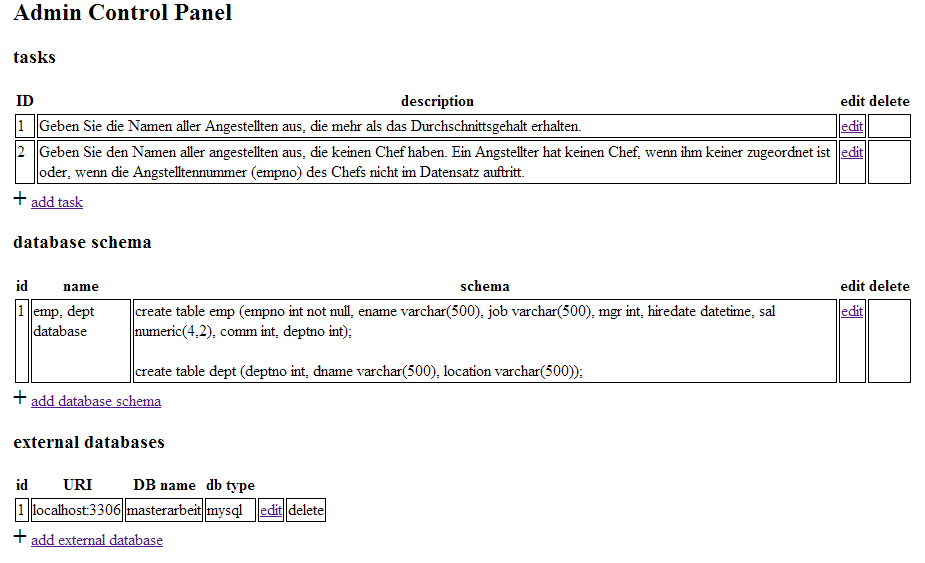
\includegraphics[scale=0.51]{Bilder/screen_acp_2.png}
\caption{Übersicht über das Admin Control Panel}
\label{fig:acp}
\end{figure}

\subsection{Datenbankschema erstellen}

Navigieren Sie auf das Admin Control Panel. Betätigen Sie den Link 'add database schema'. Daraufhin erhält die Tabelle ein weiteres Schema, was mit \verb|Empty, Empty| markiert ist. Klicken Sie auf 'edit', um das Schema anzupassen. Die erste Spalte bezeichnet den Namen des Datenbankschemas. Damit lässt es sich bei der Zuordnung zu einer Aufgabe leichter wiederfinden. In der zweiten Spalte befindet sich ein Eingabefeld. Tragen Sie hier das Schema ein. Verwenden Sie Dabei \verb|CREATE TABLE|-Anweisungen, die mit Semikolon (;) abgetrennt sind. Betätigen Sie danach den 'save'-Knopf.

\subsection{Externe Datenbank anbinden}

Die SQL-Anfragen des Lernenden und die Musterlösung werden auf externen Datenbanken zur Kontrolle ausgeführt. Um eine externe Datenbank anzubinden, navigieren Sie im Admin Control Panel auf den Link 'external databases'. Klicken Sie nun auf 'add external database' und anschließend auf 'edit'.  Tragen Sie Daten entsprechend der folgenden Tabelle in die Felder ein.

\begin{tabular}{|l|p{14cm}|}\hline
Spatel 1 & Tragen Sie hier den Hostnamen und den Port des DBMS getrennt mit Doppelpunkt (:) ein. Der Port muss auch angegeben werden, wenn es der Standard-Port ist.\\\hline
Spatel 2 & Hier wird der Name der Datenbank eingetragen.\\\hline
Spatel 3 & Tragen Sie hier ein, was sie für ein DBMS benutzen. Zur Auswahl stehen MySQL, PostgreSQL und Oracle DB.\\\hline
Spatel 4 & Hier tragen Sie den Benutzernamen für den Zugriff auf die Datenbank ein.\\\hline
Spatel 5 & Hier tragen Sie das Passwort für den Zugriff auf die Datenbank ein.\\\hline
\end{tabular}



Es muss darauf geachtet werden, dass die externe Datenbank bereits Tabellen mit Daten enthält. Der SQL-Equalizer legt auf externen Datenbanken keine Tabellen oder Datensätze an.

\subsection{Aufgabe erstellen}

Um eine neue Aufgabe einzupflegen, navigieren Sie im Admin Control Panel auf den Link 'add task' und anschließend auf 'edit'. Sie sehen nun eine neue Eingabemaske, wie sie auch in Abbildung \ref{fig:acp2} zu sehen ist. Tragen Sie die Daten entsprechend der folgenden Tabelle ein.

\begin{figure}
\centering
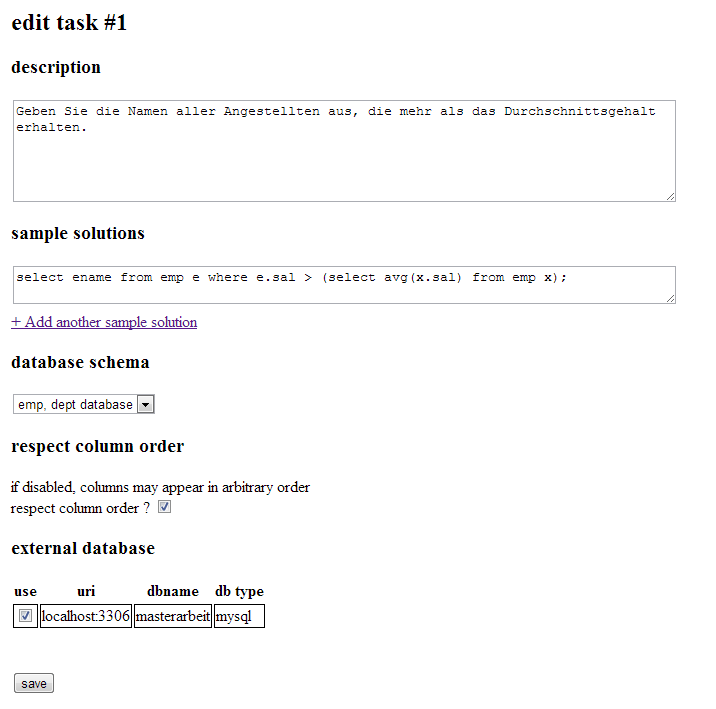
\includegraphics[scale=0.61]{Bilder/screen_acp_1.png}
\caption{Erstellen einer Aufgabe im ACP}
\label{fig:acp2}
\end{figure}

\begin{tabular}{|l|p{12cm}|}\hline
description & Tragen Sie hier die Aufgabenstellung als Textform ein. Beschreiben Sie, welche Spalten welcher Tabelle in was für einer Sortierung (falls gewünscht) ausgegeben werden sollen, so dass der Student möglichst genau weiß, was er zu tun hat.\\\hline
sample solutions & Tragen Sie hier die Musterlösung in Form einer SQL-Anfrage ein. Der Student kann diese Anfrage nicht sehen. Möchten Sie mehrere Musterlösungen verwenden, weil sie sich strukturell stark unterscheiden, so verwenden Sie den Link 'add another sample solution', um mehrere Eingabefelder zu erzeugen.\\\hline
database schema & Verwenden Sie das dropdown-Menü, um ihr erstelltes Datenbankschema hier anzugeben.\\\hline
respect column order & Haken Sie das Kästchen an, wenn die Spalten genau die angegebene Reihenfolge einhalten sollen.\\\hline
external database & Markieren Sie hier die externen Datenbanken, auf denen die Musterlösung und die Lösung des Lernenden ausgeführt werden sollen.\\\hline
\end{tabular}

Nachdem Sie den 'save'-Knopf betätigt haben, ist die Aufgabe im System eingepflegt.


\subsection{Handbuch für Anwender}

Der SQL-Equalizer ermöglicht es, das formulieren von SQL-Anfragen zu üben. Dabei melden Sie sich als Nutzer mit ihrem Browser beim SQL-Equalizer an. Sie können dann Aufgaben lösen und erhalten vom System Rückmeldung, ob ihre Lösung korrekt war oder nicht. Dabei zeigt ihnen der SQL-Equalizer in welchem Bereich ihrer SQL-Anfrage Probleme aufgetaucht sind. Sie haben dann die Möglichkeit erneute Lösungsversuche einzureichen. 

\subsubsection{Übersicht}

Nachdem Sie sich angemeldet haben, sehen Sie den Startbildschirm. Dieser ist in drei Bereiche geteilt: Im ersten Bereich sehen Sie ihre fünf letzten Einsendungen. In einer Tabelle wird Ihnen dabei das Datum der Einsendung (time), die Aufgabennummer (task), ihr SQL-Statement (sql statement) sowie die Korrektheit der Lösung (correct?) angezeigt.

Im Feld 'correct?' gibt es drei mögliche Werte: Konnte ihr SQL-Statement durch das Standardisierungsverfahren an die Musterlösung angepasst werden, so erhalten Sie dort die Ausgabe \textbf{yes}. Ist dies nicht gelungen und ihre Lösung liefert beim Ausführen auf einer externen Datenbank mit realen Daten nicht die gleichen Ergebnisse wie die Musterlösung, so erhalten Sie die Ausgabe \textbf{no}. Ansonsten erhalten Sie die Antwort \textbf{unknown}. Dabei ist zu beachten, dass ihre Lösung im dritten Fall dennoch korrekt sein kann. Dem Dozenten werden solche Lösungen angezeigt, damit dieser dann entscheiden kann, ob ihre Lösung korrekt ist oder nicht.

\begin{figure}[H]
\centering
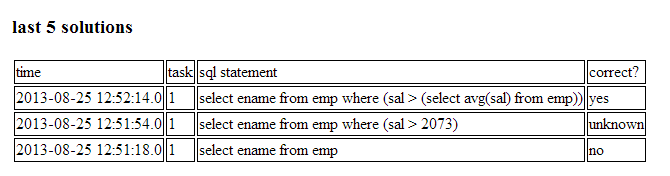
\includegraphics[scale=0.7]{Bilder/screen_user_1.png}
\caption{Informationen über die letzten fünf Lösungsversuche}
\end{figure}

Im nächsten Bereich, sehen Sie eine Statistik über alle Aufgaben. Dabei wird in einer Tabelle angezeigt, wie viele Lösungsversuche sie pro Aufgabe bisher benötigt haben (\#solutions). Weiterhin wird angezeigt, wie viele von diesen Lösungsversuchen korrekt waren (correct). Eine Erfolgsrate (ratio) und der Zeitpunkt des letzten Lösungsversuches vervollständigen die Anzeige.

\begin{figure}[H]
\centering
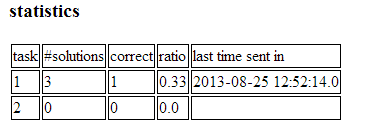
\includegraphics[scale=0.7]{Bilder/screen_user_2.png}
\caption{Statistik über alle Aufgaben}
\end{figure}

Im dritten und letzten Bereich, finden Sie eine Übersicht über alle bisher ungelösten Aufgaben. Dort werden Ihnen die Anzahl der Lösungsversuche sowie ein Hyperlink zur Aufgabe angezeigt.

\begin{figure}[H]
\centering
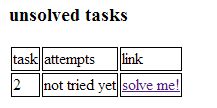
\includegraphics[scale=0.7]{Bilder/screen_user_3.png}
\caption{Ungelöste Aufgaben}
\end{figure}

\subsubsection{Einsenden einer Lösung}

Nachdem eine Aufgabe zum Lösen ausgewählt wurde, öffnet sich eine Eingabemaske. Oben sehen Sie die Aufgabenstellung in Textform. Diese enthält Informationen, welche Spalten im Ergebnis angezeigt werden sollen. Darunter befindet sich das Datenbankschema in Form von \verb|CREATE TABLE|-Anweisungen. Diesem Schema kann entnommen werden, welche Spalten in welcher Art und Weise definiert sind. Darunter befindet sich ein Eingabefeld, in das die Lösung eingetragen werden kann. Der Aufbau der Eingabemaske ist in Abbildung \ref{fig:maske1} zu sehen.

\begin{figure}[h]
\centering
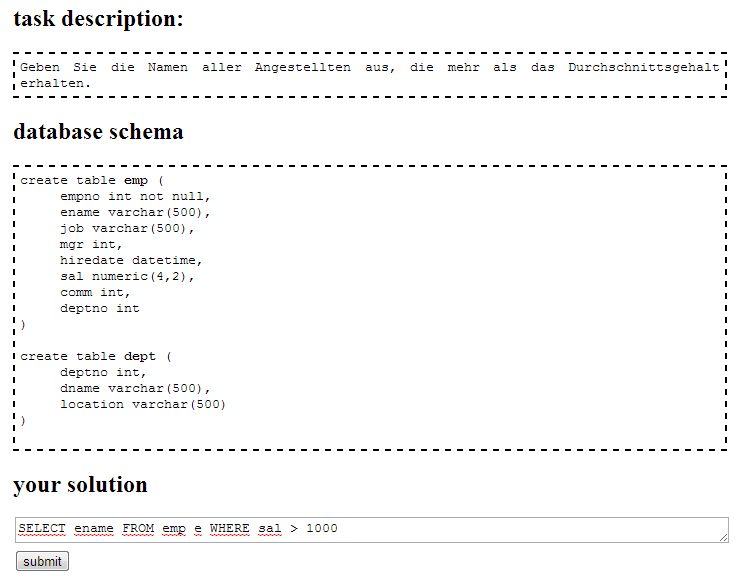
\includegraphics[scale=0.6]{Bilder/screen_user_4.png}
\caption{Eingabemaske}
\label{fig:maske1}
\end{figure}


Nachdem Sie die Lösung abgeschickt haben, gibt Ihnen der SQL-Equalizer ein detailliertes Feedback dazu. Zunächst wird die geparste Eingabe sowie - auf Wunsch - die standardisierte Eingabe angezeigt.

\begin{figure}[H]
\centering
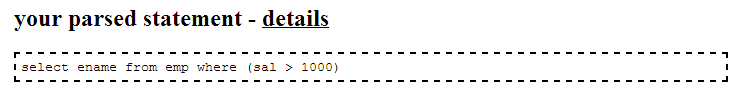
\includegraphics[scale=0.6]{Bilder/screen_user_5.png}
\caption{Geparste Eingabe}
\end{figure}

Darunter befinden sich die Kommentare des SQL-Equalizer in drei Abschnitten. Im ersten Abschnitt wird angezeigt, ob die eingesandte Lösung durch Standardisierung mit der Musterlösung übereinstimmt. Ist dies der Fall, werden alle weiteren Ausgaben unterbunden und Sie erhalten die Meldung, dass ihre Lösung korrekt ist.

Im zweiten Abschnitt werden die zwei Ergebnismengen, die von der eingesandten und der Musterlösung erzeugt worden sind, verglichen. Geben beide Anfragen die gleichen Ergebnisse zurück, wird Ihnen dies angezeigt, zusammen mit der Meldung, dass der SQL-Equalizer nicht sagen kann, ob ihre Lösung korrekt ist oder nicht. Unterscheiden sich die Ergebnismengen jedoch, wird Ihnen angezeigt, dass ihr Lösungsversuch nicht korrekt war.

Im letzten Abschnitt weist Sie der SQL-Equalizer auf Abweichungen in ihrer Lösung hin. Dabei vergleicht der SQL-Equalizer die einzelnen Teile ihrer Anfrage mit den entsprechenden Teilen der Musterlösung. Auch andere Eigenheiten ihrer beiden Anfragen werden verglichen. Das Ergebnis dieser Anzeige wird Ihnen dann in diesem Abschnitt angezeigt.

Ein Beispiel für eine solche Ausgabe sehen Sie in Abbildung \ref{fig:screen_user_1}

\begin{figure}[H]
\centering
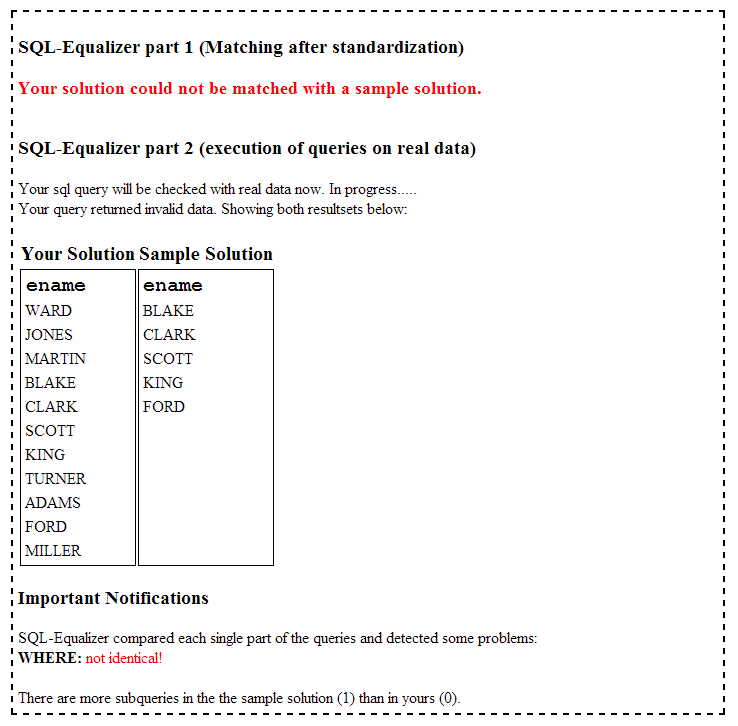
\includegraphics[scale=0.61]{Bilder/screen_user_6.png}
\caption{Rückmeldung vom SQL-Equalizer}
\label{fig:screen_user_1}
\end{figure}

Hiermit versichere ich, die vorliegende Arbeit selbstständig und unter ausschließlicher Verwendung der angegebenen Literatur und Hilfsmittel erstellt
zu haben.

Die Arbeit wurde bisher in gleicher oder ähnlicher Form keiner anderen Prüfungsbehörde vorgelegt und auch nicht veröffentlicht.

\vspace{10ex}

Halle (Saale), 24. September 2010 


\end{document}
